\documentclass[12pt, dvipdfmx]{jsbook}
\usepackage{./sty/pethesis}
\usepackage{amsmath,amssymb,bm}
\usepackage{./sty/cite}
\usepackage{minitoc}
\usepackage{hhline}
\usepackage{slashbox}
\usepackage{booktabs}
\usepackage{comment}
\usepackage{ulem}
\usepackage{url}
\renewcommand\UrlFont{\rmfamily}
\usepackage{./sty/algorithm}
\usepackage{./sty/algorithmic}
\usepackage{color}
\usepackage{latexsym}
\usepackage{ascmac}
\usepackage{breqn} % 式を途中で折り返すため
\usepackage{setspace} % 文書内の行間隔を調整
\usepackage{./sty/xbmkanji}
\usepackage[labelsep=quad]{caption}
\usepackage{otf} % UTFで指定した漢字をPDFに明記するため
\AtBeginDvi{\special{pdf:mapfile font.map}}

\makeatletter
\newcommand{\figcaption}[1]{\def\@captype{figure}\caption{#1}}
\newcommand{\tblcaption}[1]{\def\@captype{table}\caption{#1}}
\makeatother

% \usepackage[dvipdfmx, usenames]{color} %橘高追加 [usenames] → [dvipdfmx, usenames](前者は古いドライバのため,graphicxパッケージと干渉してeps以外の画像形式に対応できなくなる)

% \usepackage{subfloat}
% \usepackage[subrefformat=parens]{subcaption} %橘高追加
% \captionsetup{compatibility=false} %橘高追加
%\usepackage{otf} %橘高追加


\renewcommand{\refname}{}

\newcommand\whline{%
     \noalign{\xdef\origarrayrulewidth{\the\arrayrulewidth}%
     \global\arrayrulewidth 3\arrayrulewidth}%
     \hline%
     \noalign{\global\arrayrulewidth\origarrayrulewidth}%
}


\newcommand{\SfM}{Structure from Motion}

%%%%%%%%%%%%%%%%%%%%%%%%%%%%%%%%%%%%%%%%
\newif\iffigure
%\igurefalse
\figuretrue
%%%%%%%%%%%%%%%%%%%%%%%%%%%%%%%%%%%%%%%%

%
% 論文の表紙の項目
%
\thesistype{令和元年度 修士論文}
\title{スペクトル画像を用いた土質パラメータの推定に\\基づく建設機械の走破性判定}
\etitle{Judgement of Trafficability of Construction Machinery  \\ Based on Estimation of Soil Parameters from Spectral Images}
\affiliation{東京大学大学院 工学系研究科 精密工学専攻}
\supervisor{山下 淳 准教授}
\studentid{37-186291}
\author{山内 統広}
\begin{document}
\dominitoc
%表紙
\maketitle
%概要
%\thispagestyle{empty}
%\thispagestyle{empty}
%\chapter*{概要}
\markboth{概要}{}
\label{abst}
\def\thepage{}
\thispagestyle{empty}

人間が直接作業することの困難な環境では,ロボットを用いて作業を行うことが期待されている.このとき,作業位置を特定するなどの目的でロボットの運動を推定することが求められる.例えば,ロボットを用いた橋梁の点検では,点検箇所を把握することが必要であり,画像情報を用いたロボットの運動推定に関する研究が行われている[1].橋梁点検などのように,作業対象物に近接した状態においてより多くの情報を取得するためには,視野の限られた通常のカメラよりも視野の広いカメラが適している.本研究では,周囲360◦ の情報を一度に取得できる極めて広い視野を有する全天球カメラに注目する.\\
全天球カメラを用いた運動推定の研究として,Structurefrom Motion(SfM)による手法が提案されている[2].SfM は,カメラ1 台の移動によって異なる視点からの画像を取得し,3次元復元と運動推定を行う手法である[3].橋梁の点検においては,点検箇所を把握するために絶対的な移動距離を推定することが求められる.しかしSfM には,スケールの不定性や,カメラの移動量が小さい場合に運動推定精度が低下するという問題がある.\\
その他の運動推定の研究として,複数台のカメラを用いたステレオカメラによる3次元計測の結果を利用する運動推定の手法が提案されている[4].基線長が固定されているステレオカメラによる運動推定の性質として,上述のスケールの不定性や,カメラの移動量が小さい場合の運動推定精度の低下という問題は生じない.しかし,[4] は通常のカメラを用いており,全天球カメラの広い視野を活用したステレオによる運動推定の手法は構築されていない.\\
視野の広いカメラを複数台用いた3次元計測の研究としては,複数台の魚眼カメラを用いた手法が提案されている[5].しかし,[5] は対応点を曲線上で探索しており,また180◦ 程度の範囲のみを取得する魚眼ステレオカメラを用いて運動推定を行う場合,移動前後での計測に共通部分が含まれずに運動が推定できない場合が生じうるという問題がある.全天球カメラを用いた場合には,対応点の探索を直線上で行うことができ,またカメラがどのような移動をしても必ず共通部分が得られて運動を推定することができる.\\
本研究では,全天球ステレオカメラを用いた3次元計測結果を利用する運動推定の手法の構築を目的とする.ステレオカメラとの幾何的な関係から計測における誤差が大きいような点を,信頼度が低いとして除去することで運動推定の精度を向上させる手法を提案する.

本論文では全天球ステレオカメラの運動推定手法を構築した.
まず提案手法において基本となる2視点の画像を用いた手法について述べた.
この手法では,カメラの前に配置する透明平板の姿勢は任意とした.
しかし,この手法において透明平板をカメラの光軸と垂直に配置した場合,
特殊なケースとして扱えることが明らかとなり,その特殊性を利用して改良し,
透明平板がカメラ光軸に垂直な場合の手法として確立した.
これは平板の姿勢を任意とした場合の手法に比べ,必要な対応点数が1つ減るという特徴がある.
上述の手法はいずれも2視点間の関係のみを用いた手法であったため,
最後に前述の手法を多視点に拡張し,かつ得られた3次元情報を最適化するためのバンドル調整を用いた手法について述べた.
提案手法では屈折が発生しているため,この効果を考慮した新しい誤差関数を定義した.
なお,このバンドル調整には初期値が必要であり,前述の2視点でスケール復元が可能な手法により得られた値を初期値とした.
これにより,2視点だけでなく多視点の画像を用いて最適化が可能となり,かつ最適化処理を入れることでよりロバスト性の高い手法となった.

次に提案手法の有効性を示すため,実験を行った.
その結果,提案手法は対応点座標値の誤差に影響を受けやすいことが分かった.しかし,バンドル調整を用いた手法において,
視点の数を増やすことでこの誤差に対するロバスト性が向上することが示された.一方で,透明平板を厚くすること,解像度の高いカメラを用いることが
精度の高い計測を行うために重要であることも明らかとなった.
実画像を用いた実測実験では,実際にカメラの前に透明平板を配置した状態で撮影した画像に対して
提案手法を適用した.その結果高い精度で計測対象のスケールを復元することができ,
提案手法が有効であることが示された.

\thispagestyle{empty}

\newpage
%%%%%%%%%%%%%%%%%%%%%%%%%%%%%%%%%%%%%%%%%%%%%%%%%%%%%%%%%%%%%%%%%%%%%%%%%%%%%%%

%%%%%%%%%%%%%%%%%%%%%%%%%%%%%%%%%%%%%%%%%%%%%%%%%%%%%%%%%%%%%%%%%%%%%%%%%%%%%%%
%%% Local Variables:
%%% mode: katex
%%% TeX-master: "../thesis"
%%% End:


\frontmatter
% \input{../FrontMatter/Abstract}
%目次
\begin{spacing}{1.02} % 目次の行間隔を調整して"第3章"という記述をページの一番下から移動
\tableofcontents
\end{spacing}
%図目次
\listoffigures
%表目次
\listoftables


%以下本文
\mainmatter
\chapter{序論}
\thispagestyle{empty}
\label{ch:Introduction}
\minitoc


\newpage

%%=========================================================================================
\section{背景}\label{sec:Background}

% 最初に,章・節・項全体の内容を示す一文を入れ,そこで何の内容を述べるか読者に知らせ,準備してもらう

地震や噴火,豪雨などの自然災害はいつどこで発生するか分からず,誰もがその被害にさらされる可能性がある.
従って,自然災害の発生に備えると共に,その発生後にどのように対処するかは非常に重要である.% "そのため"は口語的,"よって"はより強く後の文章を印象図づける
特に日本は,世界のなかでも自然災害の発生頻度が高いことが知られている.
例えば地震については,日本は地震の震源が集中するプレートの境界線上に位置しており,
内閣府によると,2000年から2009年の間に世界で発生したマグニチュード6.0以上の地震のうち,約20$\%$が日本で発生した\cite{内閣府2010}.
また,日本は活火山の集中する環太平洋造山帯にも位置しているため,世界の活火山のうちの約7.2\%にあたる
111の活火山が日本に分布している\cite{内閣府2010}\cite{気象庁2019a}.
さらに,日本は世界の熱帯低気圧のうち約30\%が発生する北西太平洋に位置し,1970年から2011年にかけて,
年平均約3.8個の台風が上陸した.この上陸数は世界の中では中国,フィリピンに次いで3番目であり,世界各国に上陸する台風の約9.9$\%$に当たる\cite{廣瀬2014}\cite{気象キャスターネットワーク2014}.
このような夏から秋にかけて上陸してくる台風や,春と夏の間に日本に停滞する梅雨前線の影響で,
日本の1年間の降水量は世界平均の約2倍に達している\cite{国交省2004}\cite{気象庁2019b}.
日本と世界におけるマグニチュード6.0以上の地震,活火山,上陸した熱帯低気圧の数を,それぞれ図\ref{fig:num_disaster}(a),(b),および(c)に示す.
% % この後に土砂災害に話がいくようにするには何がより良いか

\begin{figure}[b]
	\begin{center}

		\begin{minipage}[b]{\linewidth}
		\centering
		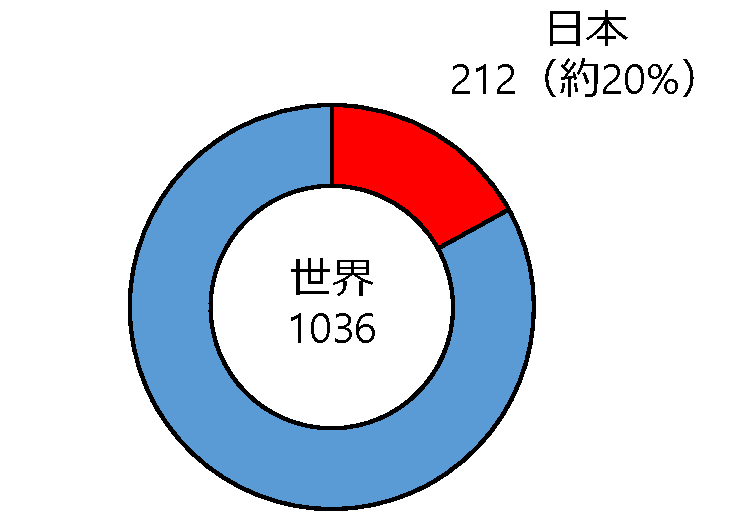
\includegraphics[width=6cm]{./Ch1_Introduction/Fig/num_japan_world_earthquake_compressed.pdf}
		\caption*{(a)マグニチュード6.0以上の地震の発生回数(\cite{内閣府2010}を参考に作成)}
		\end{minipage}

		\vspace{1cm}

		\begin{minipage}[b]{\linewidth}
		\centering
		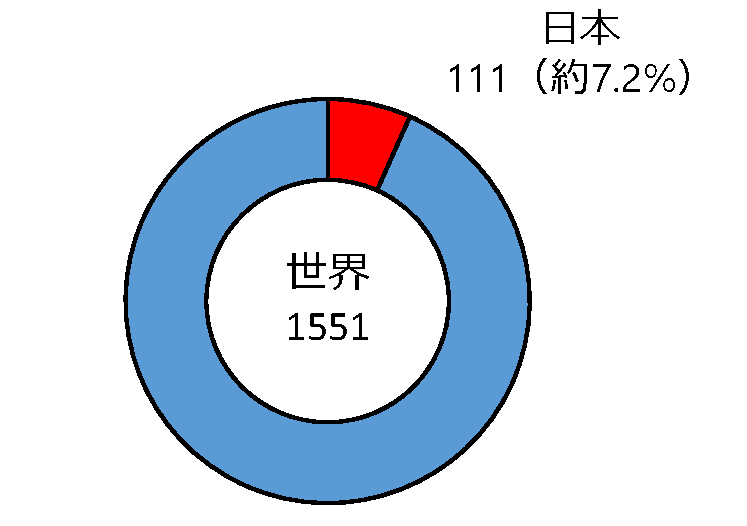
\includegraphics[width=6cm]{./Ch1_Introduction/Fig/num_japan_world_volcano_compressed.pdf}
		\caption*{(b)活火山の数(\cite{内閣府2010}を参考に作成)} 
		\end{minipage}

		\vspace{1cm}

		\begin{minipage}[b]{\linewidth}
		\centering
		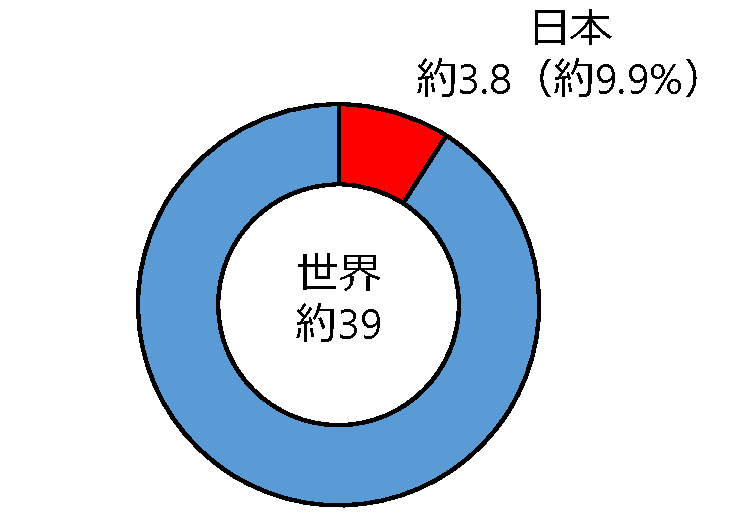
\includegraphics[width=6cm]{./Ch1_Introduction/Fig/num_japan_world_tyhoon_compressed.pdf}
		\caption*{(c)熱帯低気圧の上陸数(\cite{廣瀬2014}を参考に作成)} 
		\end{minipage}
	
	\caption{日本と世界における地震,活火山,上陸した熱帯低気圧の数}\label{fig:num_disaster}
	\end{center}
\end{figure}

\clearpage

% 土砂災害の発生件数が増加
地震,噴火,台風や梅雨前線による豪雨などの大きな自然災害は,土砂災害を誘発することが多い\cite{国交省2007}.
そのため,自然災害の頻発に伴い,土砂災害も多発している.
2008年から2018年の間に発生した土砂災害の件数を図\ref{fig:LandslideN}に示す.
このグラフに示す通り,日本においては,毎年平均1,000件ほどの土砂災害が発生している.
特に2018年には,土砂災害を伴う地震や豪雨などの自然災害が多発したため,
集計開始以降最多の3,459件の土砂災害が発生した.
例えば,2018年9月6日の早朝に発生した北海道胆振東部地震では,震源地となった北海道の胆振地方中東部を中心として広い範囲で,
合計227件の土砂災害が発生した\cite{国交省2019}.
また,2018年の6月28日から7月8日にかけて,停滞していた前線と台風第7号の影響で発生した平成30年7月豪雨でも,
西日本を中心とした全国的に広い範囲で記録的な豪雨となり,合計2,581件の土砂災害が発生した\cite{気象庁2018}.

\begin{figure}[b]
	\begin{center}	
	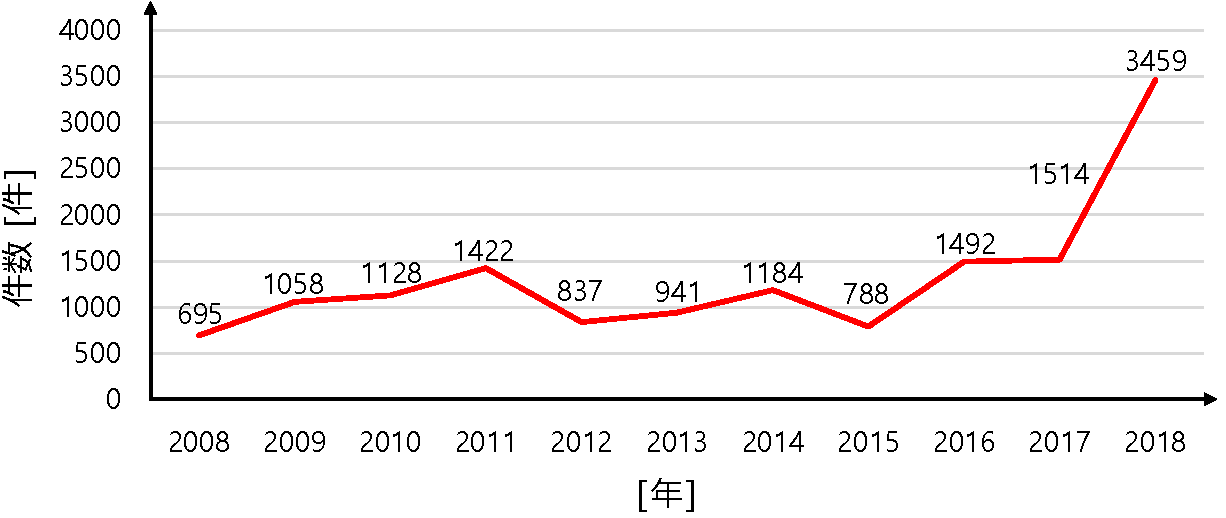
\includegraphics[width=12.5cm]{./Ch1_Introduction/Fig/土砂災害発生件数_compressed.pdf}
	\caption{土砂災害の発生件数(\cite{国交省2019}を参考に作成)}\label{fig:LandslideN}
	\vspace{3cm} % 図を文章のない部分の中心に配置するため
	\end{center}
\end{figure}

\clearpage

% 土砂災害による人的・経済的被害も増加
多発する土砂災害に伴い被害も甚大になっている.
2008年から2018年の間に発生した土砂災害に伴う被害者数と家屋被災戸数を,それぞれ図\ref{fig:LandslideDamage}(a)および(b)に示す.
図\ref{fig:LandslideDamage}(a)および(b)に示す通り,土砂災害の発生件数に比例して被害も増大しており,
2018年には被害者数,家屋被災戸数ともに過去10年間で最大となった.
先ほど言及した北海道胆振東部地震では,土砂災害に伴う死者,負傷者の数が,それぞれ36名,61名に達し,全壊した家屋も44戸に及んだ.
また,平成30年7月豪雨においては,死者,負傷者の数が,それぞれ119名,54名に達し,家屋に対する被害も,全壊364戸,半壊560戸,一部損壊470戸を記録した.
上記の具体例や図\ref{fig:LandslideDamage}(a)および(b)より,土砂災害による人的,経済的被害は無視できないほど甚大になっていることが分かる.

\begin{figure}[b]
	\begin{center}

		\begin{minipage}[b]{\linewidth}
		\centering
		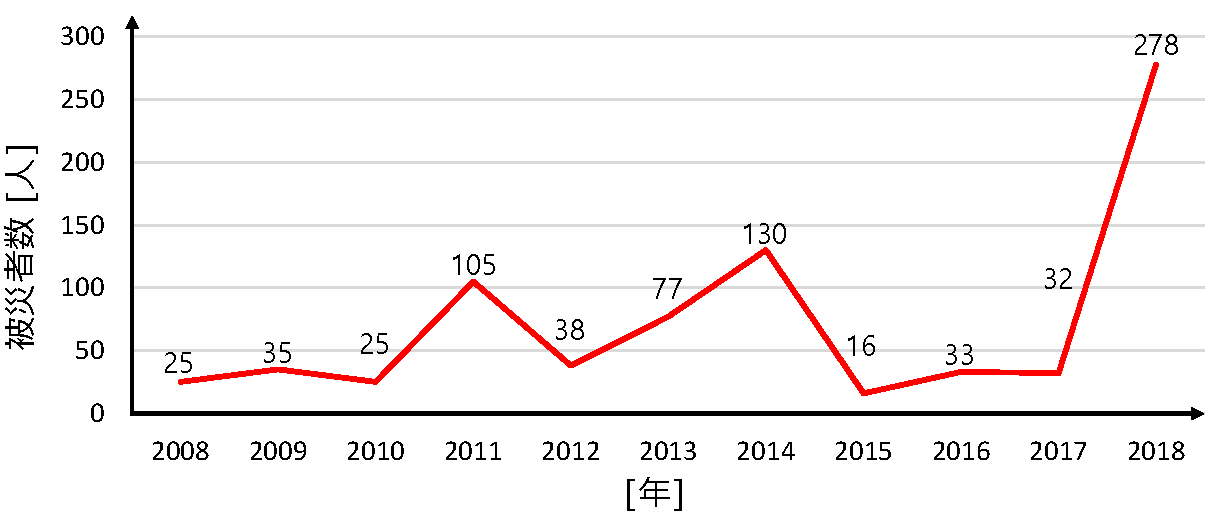
\includegraphics[width=12.5cm]{./Ch1_Introduction/Fig/土砂災害の人的被害_compressed.pdf}
		\vspace{-2mm}
		\caption*{(a)土砂災害の人的被害(死者・行方不明者・負傷者数の合計)} 
		\end{minipage}\\

		\begin{minipage}[b]{\linewidth}
		\centering
		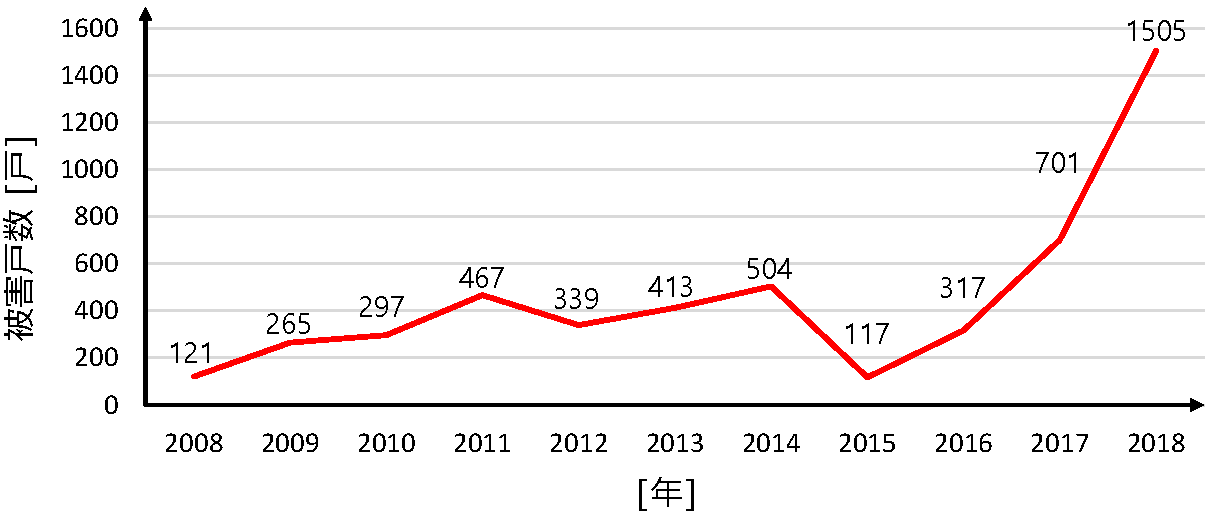
\includegraphics[width=12.5cm]{./Ch1_Introduction/Fig/土砂災害の家屋被害戸数_compressed.pdf}
		\vspace{-2mm}
		\caption*{(b)土砂災害の家屋被害戸数} 
		\end{minipage}
	
	\caption{土砂災害による被害(\cite{国交省2019}を参考に作成)}\label{fig:LandslideDamage}
	\end{center}
\end{figure}

\clearpage

土砂災害による人的,経済的被害を最小限に抑えるためには,
人命救助やライフラインの復旧などを早急に行う必要がある\cite{国交省2016}.
例えば,崩壊してきた土砂や倒壊した家屋の下敷きになった人を救助する場合には,
被災者を3日間以内に救助しなければ,生存率が大幅に低下してしまう\cite{国交省2002}\cite{生田2005}\cite{田畑2006}.
% 阪神淡路大震災の発生時からの経過日数と,救助人数のうちの生存者の割合を示す生存率の関係を図\ref{fig:death_rate_under_house}に示す.
% 図\ref{fig:death_rate_under_house}に示す通り,阪神淡路大震災が発生してから4日以上経過すると,生存率が5\%まで低下することが分かる.
また,電力,水道,通信,道路等のライフラインが土砂災害によって被害を受けた場合,
ライフラインに依存している経済活動も停滞してしまうため,経済的な損失が発生してしまう\cite{豊田2008}\cite{豊田2010}.
従って,人命救助や交通網の確保を早急に行うことは非常に重要であり,
そのためには迅速な復旧工事が必要となる\cite{国交省2016}.
そのために復旧工事において建設機械を使用する必要があるが,
土砂災害の発生した現場の地盤が軟弱な場合,
地盤が建設機械の重量に耐えられずに,建設機械が地盤にはまり込み,最悪の場合転倒する可能性がある\cite{玉手2008}\cite{玉手2014}.
軟弱な地盤にはまり込んだ建設機械を図\ref{fig:sinking_construnction_machine}に示す.
図\ref{fig:sinking_construnction_machine}の画像に示したように建設機械が軟弱な地盤にはまり込むと,
最悪の場合その場で転倒してしまう.
そのような地盤で建設機械を使用することは出来ない.
% 建設機械の使用と建設機械の転倒は直接反するわけではないが,建設機械の転倒から建設機械を使用できないということが伝わるので,"しかし"でOK
従って,復旧工事を行うためには,災害現場において建設機械の走破性を事前に判定することが重要となる.

\begin{figure}[b]
	\begin{center}
	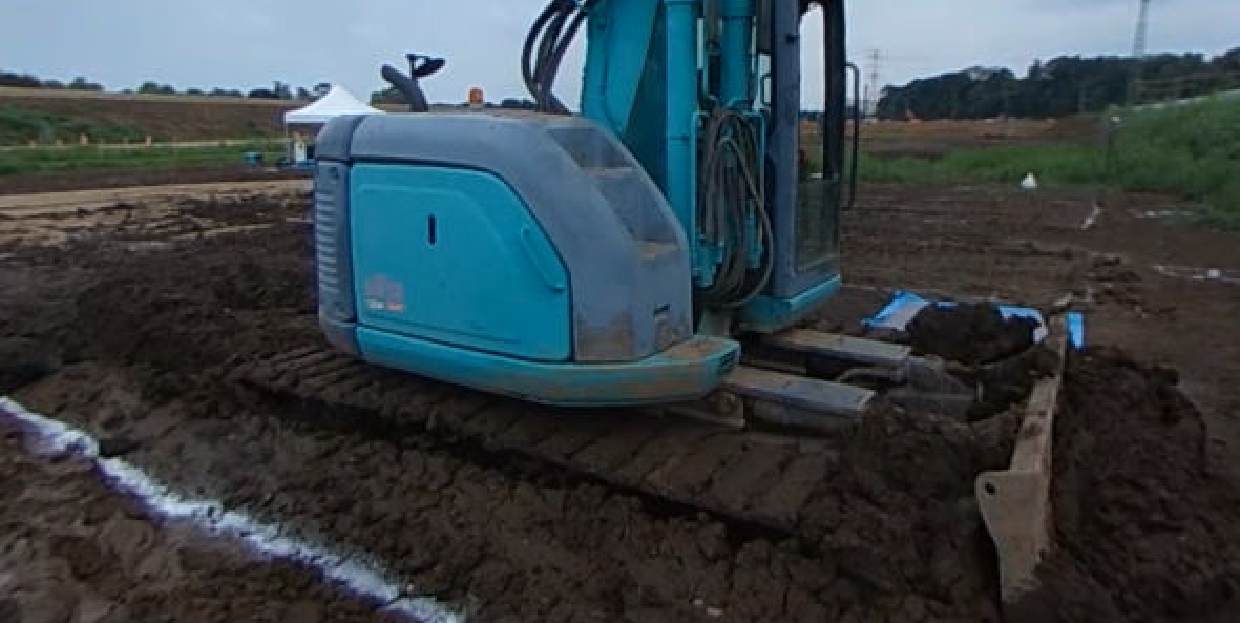
\includegraphics[width=13cm]{./Ch1_Introduction/Fig/trafficability_coneindex_72_72_compressed.pdf}
	\caption{軟弱な地盤にはまり込んだ建設機械(2019年8月28日撮影.詳細は\ref{sec:ConeindexEstimationExperiment}節に記載)}\label{fig:sinking_construnction_machine}
	\vspace{1cm} % 図を文章のない部分の中心に配置するため
	\end{center}
\end{figure}



\clearpage


%%=========================================================================================
\section{先行研究}\label{sec:PreviousStudy}

% 基本的には時制を統一

\subsection{走破性を判定する従来手法}\label{ssec:TraditionalMethod}

建設機械の走破性を判定する従来手法には,走破性の高さを示す指標の1つであるコーン指数を計測する手法がある\cite{Mulqueen1977}\cite{Perumpral1987}.
コーン指数とは,コーンペネトロメータと呼ばれる器具を現場の地面に挿入し,その際に発生する土の抵抗を,% "抵抗力"という言葉はウイルス想起させる
コーンペネトロメータの上部についているダイヤルゲージで読み取ることで得られる値である.
土の抵抗力が強いほど建設機械の走破性が高いので,
コーン指数が高いほど建設機械の走破性が高いと判定できる.
コーンペネトロメータとそれを用いたコーン指数の測定の様子を,それぞれ図\ref{fig:ConeIndexMeasurement}(a)および(b)に示す.
図\ref{fig:ConeIndexMeasurement}に示す通り,これまでコーン指数の測定は人の手で行われてきた.
しかし,災害現場では2次災害の危険が存在するため,
現場で人がコーンペネトロメータを挿入してコーン指数を測定することは大変危険である.
従って,災害現場における建設機械の走破性を判定するためには,
% 無人でコーン指数を測定するすることによって,
遠隔で走破性を判定する必要がある.

\begin{figure}[p]
	\begin{center}
		\begin{tabular}{c} % 隣り合う図がずれないようにする

			\begin{minipage}[b]{0.45\linewidth}
			\centering
			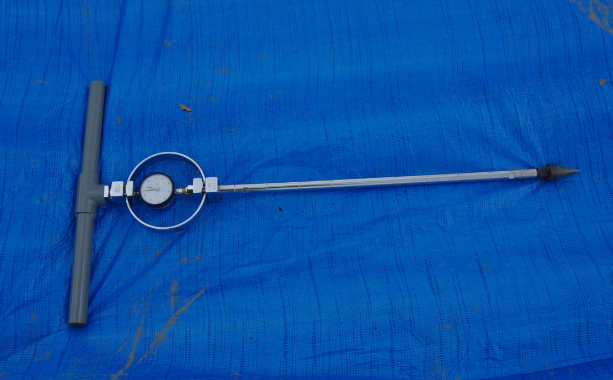
\includegraphics[width=8cm, angle=-90]{./Ch1_Introduction/Fig/コーンペネトロメータa.PNG}
			\setlength{\captionmargin}{30pt}\caption*{(a)コーンペネトロメータ\protect\linebreak(2019年8月28日撮影)}
			\end{minipage}

			\hfill

			\begin{minipage}[b]{0.45\linewidth}
			\centering
			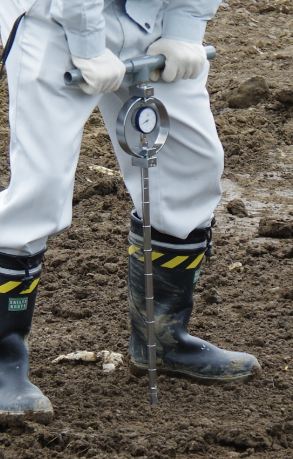
\includegraphics[height=8cm]{./Ch1_Introduction/Fig/コーンペネトロメータb.PNG}
			\setlength{\captionmargin}{20pt}\caption*{(b)コーン指数の測定の様子\protect\linebreak(2019年8月28日撮影)}
			\end{minipage}

		\end{tabular}
	\caption{コーンペネトロメータを用いたコーン指数の測定}\label{fig:ConeIndexMeasurement}
	\end{center}
\end{figure}

\clearpage

\subsection{遠隔で走破性を判定する手法}\label{ssec:UnmannedMethod}

遠隔で走破性を判定するためには,遠隔でコーン指数を測定する必要がある.
遠隔でコーン指数を測定する先行研究には,
% ロボットにコーン指数を測定する器具を搭載し,% "~には"という文言で統一
コーン指数を測定する器具を搭載したロボットを遠隔操作で対象とする環境まで移動させ,搭載した器具でコーン指数を測定する
手法が提案されている\cite{RobotWatch2002}\cite{Zacny2010}\cite{Chhaniyara2012}\cite{古谷2016}.
この手法は,人の手によるコーン指数の測定を,遠隔操作できるロボットに
置き換えることによって遠隔でのコーン指数の測定を達成している.
しかし,コーン指数の測定器具を測定地点に1カ所ずつ接触させる必要があるため,
地盤が軟弱な場合や急勾配の斜面がある場合など,対象とする環境にロボットを移動させることができない場合には,
コーン指数の測定が不可能となるという問題がある.
ロボットを対象とする環境に移動させることができない場合でも
走破性を判定するためには,
% 非接触でのコーン指数推定によって
非接触で走破性を判定する必要がある.

\subsection{非接触で走破性を判定する手法}\label{ssec:NonContactMethod}

非接触で走破性を判定するためには,非接触でコーン指数を推定する必要がある.
非接触でコーン指数を推定する先行研究には,
水が光を吸収する近赤外の波長帯を撮影した画像を用いてコーン指数を推定する手法が提案されている\cite{Rankin2010}\cite{Fernandez2015}.
この手法は,土に含まれる水の量が増加すると,一般的にコーン指数が減少することを利用している.
土に含まれる水の量が増加すると,水は近赤外の光を吸収するため土から反射してくる近赤外の光の強さは減少し,同時にコーン指数も減少する.
従って,土から反射してくる近赤外の光の強さとコーン指数は相関関係にあるため,
土の近赤外の光の強さからコーン指数をある程度推定することができる.
% この手法は,コーン指数が土に含まれる水の量に大きく影響されることと,
% 水が近赤外の光を吸収することを利用し,
% 土中の水の量が増加するのに伴い,土からの近赤外の光の強さは減少し,一般的にはコーン指数が減少するため,
この手法は,近赤外の波長帯を撮影した画像を用いて土からの近赤外の光の強さを測定することによって,非接触でのコーン指数の推定を達成している.
しかし,この手法は,土に含まれる水の量を示す指標である含水比にのみ注目し,
含水比以外でコーン指数に影響を与える土の種類には注目していないため,コーン指数の推定精度が低いという問題がある.

一方,スペクトル画像から得られた分光反射率スペクトルを用いてコーン指数を非接触で推定する手法も提案されている\cite{Kruse2000}\cite{Sopher2016}.
この手法は,コーン指数が土の種類に大きく影響されることと,
土の種類によって分光反射率スペクトルが異なることを利用している.
土の種類ごとにそれぞれ固定の分光反射率スペクトルが存在し,コーン指数も異なるため,
分光反射率スペクトルからコーン指数をある程度推定することができる.
しかし,この手法のように,固定された分光反射率スペクトルを用いて物質の種類を識別する際には,
外部の状況によって左右されない分光反射率スペクトルを用いるため,
土に含まれる水の量などの外部の状況によって変動する部分の分光反射率スペクトルは使用されない\cite{Shaw2003}.
この手法においても,水が光を吸収するため水の量によって変動する近赤外の分光反射率スペクトルは使用されていない.
従って,
% この手法は水が光を吸収する波長帯を除いた分光反射率スペクトルを用いてコーン指数を推定しているため,% 同じこと言っている
結果的に土の種類にのみ注目し,
含水比には注目していないことになる.
よって,この手法においてもコーン指数の推定精度が低いという問題が残る.

\ref{ssec:TraditionalMethod}項,\ref{ssec:UnmannedMethod}項,およびこの\ref{ssec:NonContactMethod}項で
解説した,コーン指数に基づく走破性の判定手法とその特徴を,表\ref{tbl:traditional_and_previous_method}に示す.
% 表\ref{tbl:traditional_and_previous_method}において,左の列から順に,\ref{ssec:TraditionalMethod}項,\ref{ssec:UnmannedMethod}項,
% \ref{ssec:NonContactMethod}項で解説した手法の,それぞれの場合における
表\ref{tbl:traditional_and_previous_method}より,\ref{ssec:TraditionalMethod}項や\ref{ssec:UnmannedMethod}項で
解説した手法では,土砂災害の発生現場で考慮する必要のある,2次災害や,軟弱または急勾配な地盤に対応できないため,
土砂災害の発生現場で使用するには不適切である.一方,2次災害や,軟弱または急勾配な地盤に対応できる\ref{ssec:NonContactMethod}項で
解説した手法では,コーン指数の推定精度が低いという問題がある.
そこで,土砂災害の発生現場で高精度な走破性判定を行うためには,この\ref{ssec:NonContactMethod}項で
解説した,画像を用いたコーン指数の推定において,コーン指数の推定精度を向上させる必要があることが分かる.
% 上記に示した通り,画像を用いてコーン指数を推定する
先ほど解説した通り,画像を用いてコーン指数を推定する先行研究では,コーン指数に大きく影響する土の種類と含水比のどちらか一方のみに
注目した手法が目立つ.
そこで,先行研究よりもコーン指数推定の精度を向上させるためには,土の種類と含水比の双方に注目する必要がある.

\begin{figure}[b]
	\begin{center}
	\tblcaption{走破性を判定するための従来手法と先行研究の特徴}\label{tbl:traditional_and_previous_method}
	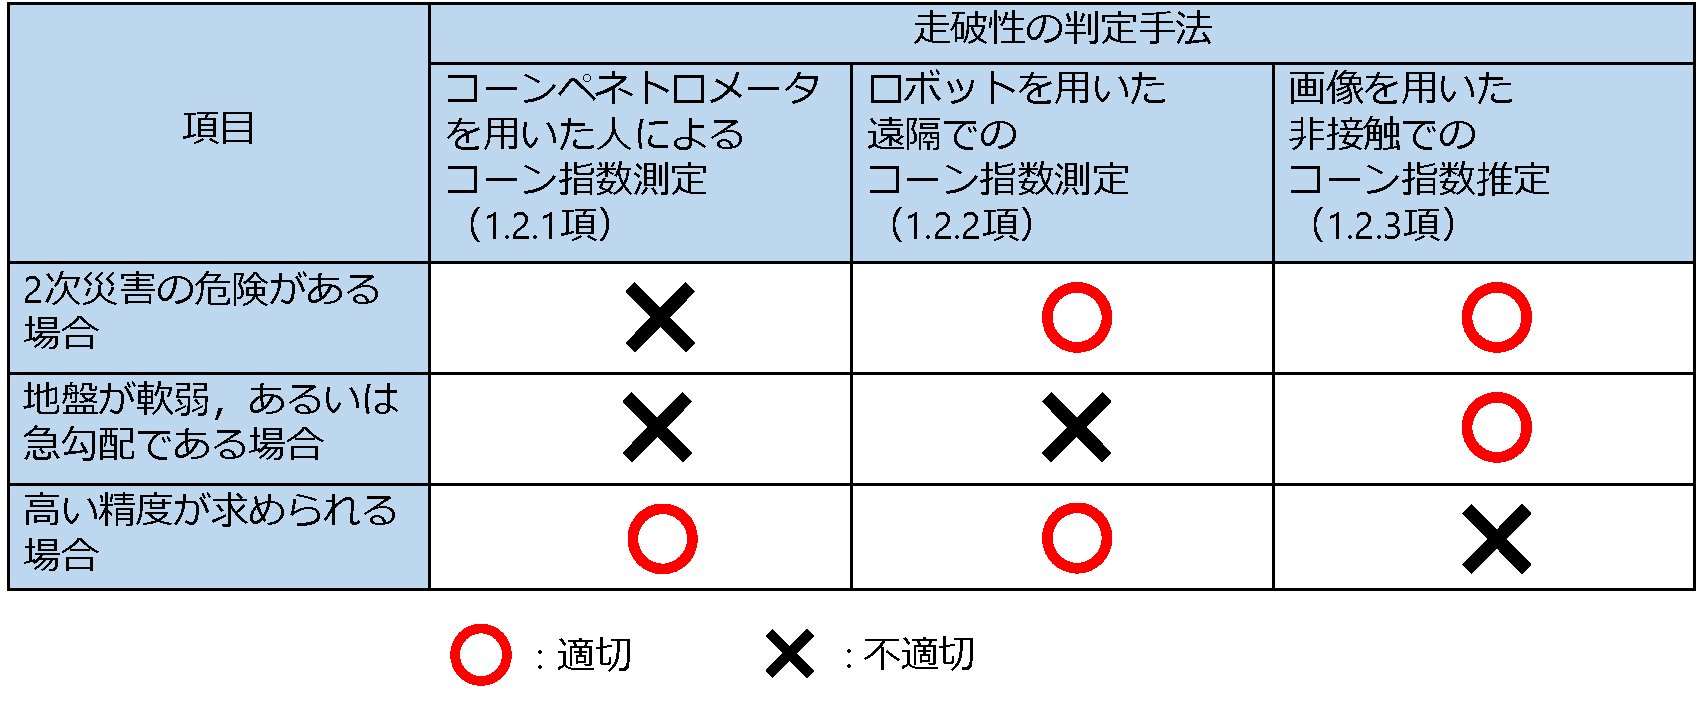
\includegraphics[width=13cm]{./Ch1_Introduction/Fig/traditional_and_previous_method_compressed.pdf}
	\vspace{1cm} % 図を文章のない部分の中心に配置するため
	\end{center}
\end{figure}

\clearpage


%%=========================================================================================
\section{本研究の目的}\label{sec:Objective}

\ref{sec:Background}節において,土砂災害が発生した災害現場では,建設機械を使用する前に走破性を判定する必要があることを述べた.
次に,\ref{sec:PreviousStudy}節において,災害現場での走破性の判定には,
非接触での走破性判定が求められており,
そのために非接触でコーン指数を推定する必要があることを述べた.
また,コーン指数には土の種類と含水比の双方が大きく影響しているため,双方に注目する必要があるが,
従来の非接触でコーン指数を推定する手法には,双方に注目した手法が確認されていないことにも言及した.
そこで,本研究の目的を以下の通りとする.

\vspace{5pt}
\begin{itembox}[c]{目的}
\begin{center}
土の種類と含水比の双方に注目した\\非接触での建設機械のための走破性判定
\end{center}
\end{itembox}
\vspace{5pt}

% 提案手法の概要
本研究においては,まず非接触で土の種類の識別と含水比の推定を行い,
それらを用いてコーン指数を推定することによって,非接触での走破性判定を行う.
また,土の種類の識別と含水比の推定を非接触で行うために,
スペクトル画像という画像を用い,そこから取得する分光反射率スペクトルを用いる.

\clearpage

%%=========================================================================================
\section{本論文の構成}\label{sec:Structure}

本論文は,全6章から構成されている.
本論文の構成を\mbox{図\ref{fig:MThesisConstitution}}に示す.

第\ref{ch:Introduction}章では,土砂災害の発生現場における建設機械の走破性の判定の必要性と,
そのために非接触での走破性判定が必要であることを述べた.
従来の非接触での走破性判定においては,走破性を示す指標の1つであるコーン指数を非接触で推定していた.
しかし,その手法では,コーン指数に大きな影響を与える
土の種類と含水比の双方に注目した手法は確認されていないことにも言及した.
そこで,本研究における目的を,土の種類と含水比の双方に注目した非接触での走破性判定とすることを述べた.
そのために,スペクトル画像から取得する分光反射率スペクトルを用いて
土の種類の識別と含水比の推定を行い,その2つからコーン指数を推定するという提案手法について簡単に解説した.
% 非接触での走破性判定:目的
% 画像を用いたコーン指数の推定:手段
% "実施"ではなく"行う"という文言に統一

第\ref{ch:PrinciplesOfMethod}章では,
非接触での走破性判定のために本研究で提案した,
スペクトル画像から土の種類の識別と含水比の推定を行い,その2つを用いてコーン指数を
推定する手法で利用する原理について述べる.
まず,分光反射率スペクトルを用いた土の種類の識別と含水比の推定で利用する原理と,
その土の種類と含水比からコーン指数を推定する際に利用する原理の2つについて解説する.% "~の原理"という用例が多い
次に,分光反射率スペクトルを取得するスペクトル画像について述べる.% "~について述べる"という用例で基本的には統一
最後に,スペクトル画像を用いて推定したコーン指数による,
非接触での走破性判定の有効性について議論する.

第\ref{ch:SoilTypeDiscrimination}章では,
非接触での走破性判定のために本研究で提案した手法の最初のステップである,
スペクトル画像を用いて土の種類を識別するステップの詳細について述べる.
まず,本研究では,土の種類ごとに分光反射率スペクトルが異なることを利用し,
スペクトル画像から取得した分光反射率スペクトルを用いて土の種類を識別することを述べる.
次に,多くの土の種類を分光反射率スペクトルから識別するためには,
% 波長分解能の高い
非常に多くの波長帯の光の強さを記録する分光反射率スペクトルを取得する必要があることに言及し,
それを取得するためには,入射光を分光させてその強さを記録した波長帯の幅を狭くした,
波長分解能の高いスペクトル画像が必要となることを述べる.
% 土の種類を識別するためには波長分解能の高い詳細な分光反射率スペクトルを取得する必要がある.
そのために,本研究では,一般的なRGB画像が取得するR,G,Bの3波長帯以外の波長帯も取得するマルチスペクトル画像のなかでも,
波長分解能の高いマルチスペクトル画像を土の種類の識別に使用することを述べる.
最後に,上記で解説した,スペクトル画像を用いて土の種類を識別するステップの有効性を確認するために実施した
検証実験とその結果について解説と考察を行う.

第\ref{ch:WaterContentEstimation}章では,
非接触での走破性判定のために本研究で提案した手法の2番目のステップである,
スペクトル画像を用いて含水比を推定するステップの詳細について述べる.
まず,本研究では,水が近赤外の光を吸収することを利用し,
スペクトル画像から取得した近赤外の波長帯と水が光を吸収しない波長帯の,2つの波長帯の分光反射率の差を用いて% "水が光を吸収する・しない"という用例で基本的には統一し,"吸光波長帯"という単語は使用しない.
含水比を推定することを述べる.
次に,水は近赤外の広い範囲の光を吸収するため,近赤外の広い範囲を1つの波長帯で取得する必要があることに言及し,
近赤外の広い範囲を1つの波長帯で取得するためには,幅が広い波長帯を取得できるようにしたスペクトル画像が必要となることを述べる.
そのために,本研究では,スペクトル画像のなかでも,
光の強さを記録する波長帯の数が比較的少数である代わりに,1つ1つの波長帯の幅を広くとることができるため,
近赤外の広い範囲を1つの波長帯で取得できる
マルチスペクトル画像を使用することを述べる.
最後に,上記で解説した,スペクトル画像を用いて含水比を推定するステップの有効性を確認するために実施した
検証実験とその結果について解説と考察を行う.

第\ref{ch:ConeIndexEstimation}章では,
非接触での走破性判定のために本研究で提案した手法の最後のステップである,
識別した土の種類と推定した含水比からコーン指数を推定するステップの詳細について述べる.
まず,本研究では,土の種類と含水比が分かればコーン指数が推定可能であることを利用し,
第\ref{ch:SoilTypeDiscrimination}章で識別した土の種類と
第\ref{ch:WaterContentEstimation}章で推定した含水比から
コーン指数を推定することを述べる.
次に,土の種類と含水比からコーン指数を推定するためには,土の種類ごとの含水比とコーン指数の関係を予め把握する必要があることに言及し,% "含水比","コーン指数"という順番
そのために,予め土の種類ごとに含水比を変えてコーン指数を測定し,
土の種類によって異なる含水比とコーン指数の関係を記録することを述べる.
最後に,上記で解説した,識別した土の種類と推定した含水比からコーン指数を推定するステップの有効性を確認するために
屋外の工事現場で実施した検証実験とその結果について解説と考察を行う.

第\ref{ch:Conclusion}章では,本論文の結論と今後の展望を述べる.

\begin{figure}[p]
	\begin{center}
	\centering
	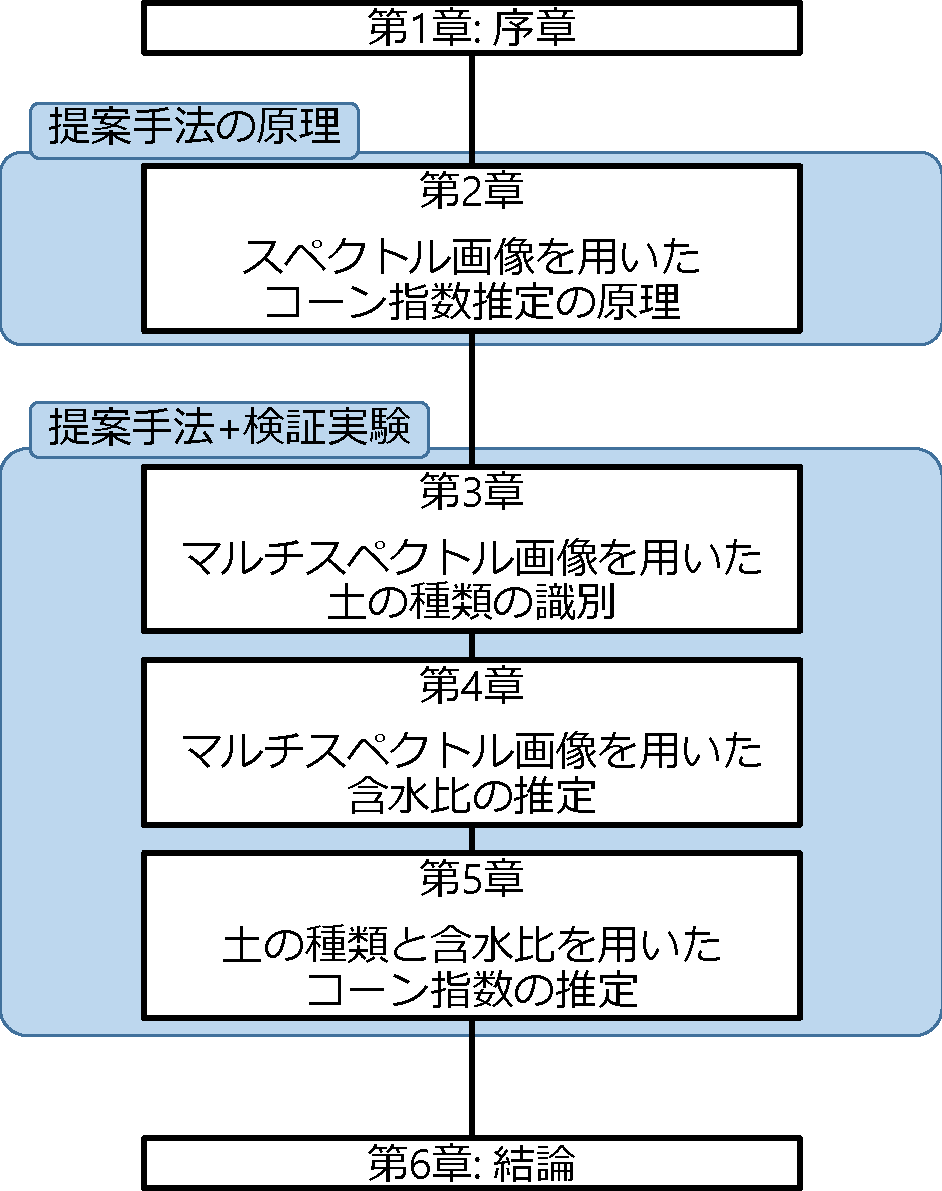
\includegraphics[width=8cm]{./Ch1_Introduction/Fig/thesis_constitution_compressed.pdf}
	\caption{修論構成}\label{fig:MThesisConstitution}
	\end{center}
\end{figure}

\clearpage


%%%本文終了
\chapter{スペクトル画像を用いた非接触でのコーン指数推定の原理}
\thispagestyle{empty}
\label{ch:PrinciplesOfMethod}
\minitoc

\newpage
%%%%%%%%%%%%%%%%%%%%%%%%%%%%%%%%%%%%%%%%%%%%%%%%%%%%%%%%%%%%%%%%%%%%%%%%%%%%%%%

%==============================================================================
\section{はじめに}

本章では,非接触での走破性判定のために本研究で提案した,スペクトル画像を用いたコーン指数推定で利用する原理の詳細について解説する.

まず,\ref{sec:PrimciplesOfConeindexEstimation}節においては,
走破性を示す指標であるコーン指数を,土の他の性質を示す指標から推定する際に利用する原理について述べる.
本研究では,建設機械の走破性が,土の基礎的な性質に大きく影響されることを利用し,
コーン指数を,
% 土の基礎的な性質を示す
土の種類と含水比から推定する.

% "土の種類"という単語と"含水比"という単語を用いる
\ref{sec:SpectrumAndMaterialRelationship}節においては,
コーン指数を推定するために使用する土の種類と含水比を,非接触で推定する際に利用する原理について述べる.
本研究では,物質の種類と状態によって分光反射率スペクトルが変化することを利用し,
分光反射率スペクトルを用いて土の種類と含水比を推定する.
% 本研究では,土の種類と含水比を非接触で推定することで非接触での走破性判定を達成する.

\ref{sec:SpectrumFromSpectralImage}節においては,
分光反射率スペクトルをスペクトル画像から取得する手法の詳細について述べる.
本研究では,建設機械が通れる程度の面積の分光反射率スペクトルを取得するために,
広い面積の分光反射率スペクトルを取得できるスペクトル画像を用いる.

最後に,\ref{sec:Ground}節においては,
本研究で走破性判定の対象とする一般的な地盤について解説する.
次に,画像を用いることによって,
地盤の深い部分の土の情報を使用せずに表面の土の情報のみを使用して推定したコーン指数を
用いて判定した走破性の有効性について議論する.
% "地盤"と"土"という単語を使い分ける

\newpage


%==============================================================================
%土質パラメータによるコーン指数推定の原理
%==============================================================================
\section{土質パラメータによるコーン指数推定の原理}
\label{sec:PrimciplesOfConeindexEstimation}

\subsection{土質パラメータ}
\label{ssec:SoilParameters}

% まず最初に,土の性質を示す土質パラメータについて解説
土には様々な性質があり,その性質の程度を示すための指標が複数存在する.
例えば,土における植物の育ちやすさを示す指標としては土のpH値があり,
pH値が低い酸性の土では植物が育ちにくいことが知られている\cite{三枝1991}\cite{図子1993}.
% 土のpH値の測定方法,説明
% pH値が低い酸性の土では植物が育ちにくいことが知られている.
また,地震によって液状化が発生する際の液状化の激しさの程度を示す指標としては
地盤液状化指数があり,
地盤液状化指数が大きいほど液状化が発生した時の構造物への被害は大きなることが知られている\cite{龍岡1980}\cite{岩崎1980}\cite{浜田1986}.
% 地盤液状化指数の測定方法
% 一般的には地盤液状化指数が大きい地盤ほど
% 液状化が発生した時の構造物への被害は大きくなる.
その他にも,斜面の安定性などの様々な土の性質を示す指標が存在する\cite{三笠1964}.
このような土の性質の程度を示す指標のことを土質パラメータと言う\cite{山口1986}\cite{渡部2007}.
多くの土の性質は土の有する他の性質から影響を受けるため,土質パラメータも他の土質パラメータから大きな影響を受けることが多い\cite{太田1988}\cite{三隅1992}.
このような土質パラメータのうちの1つに,走破性の高さを示す指標であるコーン指数という土質パラメータが存在する.

\subsection{コーン指数}
\label{ssec:Coneindex}

% そのうちの1つであるコーン指数が,走破性の高さを示す指標であることを述べた
\ref{ssec:SoilParameters}項で述べたように,土質パラメータのうちの1つに,不整地の上を走る車両の走破性の高さを示すコーン指数という土質パラメータが存在する.
コーン指数は,1948年にアメリカ陸軍工兵隊で開発されたコーンペネトロメータという器具を使用して測定する指標である\cite{WES1948}\cite{Perumpral1987}.
当時開発されたコーンペネトロメータは,長さ91.4cm, 直径0.95cmのシャフトに,先端角$30^\circ$,底面の面積が1.61$\rm cm^2$の円錐状のコーンを
つけ,シャフトの円錐状のコーンをつけた側とは反対側に土の抵抗を測定するためのゲージとハンドルを搭載していた.
使用方法は,
最初にゲージの値を0に合わせた後,
シャフトを円錐状のコーンの付いた方から地面に挿入し,その際の抵抗を上部のゲージで読み取って,
その値からシャフトの先端についているコーンの底面の面積を割り,一定の係数をかけることでコーン指数が算出される.
コーンペネトロメータは持ち運びが容易なため,
走破性を判定する以外にも様々な用途に使用されるようになり,
その用途に合わせてコーンペネトロメータの寸法も変化し,多くの派生型が作成された\cite{Hendrick1969}\cite{Prather1970}.
% 派生型の説明 \cite{Perumpral1987}から孫引き
\ref{ssec:SoilParameters}項で述べたように,多くの土の性質と同じく走破性は土の有する他の性質から影響を受けるため,
走破性を示す指標であるコーン指数も他の土質パラメータから大きな影響を受ける.

\subsection{コーン指数以外の土質パラメータからのコーン指数の推定}
\label{ssec:ConeindexEstimation}

走破性に影響を与える他の土の性質として,% 土の性質は走破性,土質パラメータはコーン指数に影響を与える
土の粒子の材質や直径の分布,形,表面の粗さ,土に含まれる水の量などの基礎的な土の性質を挙げることができる\cite{小田1971}\cite{Okello1991}\cite{Shoop1993}\cite{Flores2014}.
それらを示す指標としては,土の粒子の鉱物組成,有機物含有量,粒度分布,球形率,含水比が挙げられる.% それぞれの指標の説明 "定量化した"ではなく"示す"指標という表現に統一
% それぞれの土質パラメータの測定方法を引用
従って,土質パラメータの土の粒子の鉱物組成,有機物含有量,粒度分布,球形率,含水比は
走破性の指標であるコーン指数に大きな影響を与える\cite{Collins1971}.% 引用
つまり,これらの基礎的な土の性質を示す土質パラメータが分かれば,コーン指数も一意に決まる\cite{Ayers1982}\cite{Jenkins1985}\cite{Elbanna1987}\cite{Mulhearn2001}.

上記の基礎的な土の性質を示す土質パラメータのうち,外部の状況に左右されない土に固有の土質パラメータである土の粒子の鉱物組成,有機物含有量,粒度分布,球形率が
同じ土を同じ種類の土であると定義すると,
コーン指数に大きな影響を与える残りの土質パラメータは含水比のみとなる.
従って,
土の種類と含水比が分かれば,コーン指数は一意に決まる.

そこで本研究では,
% 上記で述べた土の種類と含水比のコーン指数との関係を利用することによって,
上記で述べたコーン指数と基礎的な土の性質を示す土質パラメータの関係を利用することによって,
土の種類と含水比から
コーン指数の推定を行う.

\clearpage

%==============================================================================
%分光反射率スペクトルでの土質パラメータ推定の原理
%==============================================================================
\section{分光反射率スペクトルでの土質パラメータ推定の原理}
\label{sec:SpectrumAndMaterialRelationship}

\subsection{分光反射率スペクトル}
\label{ssec:Spectrum}

物質は,その分子や原子の構造,または物質を構成する微粒子の大きさや形,表面の凹凸によって,
光の波長ごとの反射,散乱,吸収,そして放射の度合いが異なる\cite{Shaw2002}\cite{Shaw2003}.
従って,物質の種類と状態によって,分光反射率スペクトルが異なる.
分光反射率スペクトルとは,下の式のように,物質に入射してくる光のエネルギーに対して,
その物質が反射した光のエネルギーの割合を波長ごとに並べたものである.% 引用
分光反射率を示す式は,
\begin{eqnarray}
\rho(\lambda) = \frac{L_s(\lambda)}{L_i(\lambda)},\label{eq:reflectance_spectrum_caliculation}
\end{eqnarray}
となる.\mbox{式(\ref{eq:reflectance_spectrum_caliculation})}において,$\rho(\lambda)$は物質の分光反射率を,
$L_s(\lambda)$は物質が反射する光の強さを,そして$L_i(\lambda)$は物質に入射する光の強さをそれぞれ示す.
また,$\lambda$は波長を示す.%$\rho(\lambda)$,$L_s(\lambda)$,$L_i(\lambda)$は波長の関数である.

この分光反射率スペクトルを使用することによって,物質の種類の識別と状態の推定を非接触で行うことが可能である.
例えば,化学や物理学の分野では分光反射率スペクトルが物質の識別などに使用されている\cite{長田2004}.
% もっと具体的な例を追加

% \mbox{式(\ref{eq:r})}

\subsection{非接触での土質パラメータの推定}
\label{ssec:NonContactEstimation}

分光反射率スペクトルを用いて土質パラメータを非接触に推定することも可能である.
例えば,土のpH値の推定や,含水比の推定などに使用されている\cite{Ben-Dor2002}\cite{Rossel2006}.%\cite{McCarty2002}\cite{Cozzolino2003}.% 引用ごとの例を解説
また,土の種類に含めた,外部の状況に左右されない土に固有の土質パラメータである土の粒子の鉱物組成,有機物含有量を推定することも可能である\cite{Ben-Dor1995}\cite{Janik1998}.
さらに,粒度分布も分光反射率スペクトルに影響を与えることが分かっている\cite{小嶋1996}.
従って,分光反射率スペクトルを用いて,コーン指数に大きな影響を与える土の種類と含水比を推定することが期待できる\cite{小川1989}\cite{Jia2017}.
% "可能である"と"できる"を使用

\clearpage

%==============================================================================
%スペクトル画像からの分光反射率スペクトルの取得
%==============================================================================
\section{スペクトル画像からの分光反射率スペクトルの取得}
\label{sec:SpectrumFromSpectralImage}

\subsection{スペクトル画像}
\label{ssec:SpectralImage}

\ref{sec:SpectrumAndMaterialRelationship}節で述べた通り,本研究では,分光反射率スペクトルを用いることによって,
土の種類の識別と含水比の推定を非接触に行う.
この土の種類と含水比を用いてコーン指数を推定することによって,建設機械のための走破性の判定を非接触に行うことが可能になると期待できる.

建設機械の走破性を判定するためには,対象となる建設機械が走行できる程広い面積の土のコーン指数を推定する必要がある.
それ程広い面積のコーン指数を推定するためには,
% コーン指数に大きな影響を与える土質パラメータも
コーン指数に大きく影響する土の種類の識別と含水比の推定に用いる分光反射率スペクトルを
広範囲で測定しなければならない.
% しかし,これまでの分光反射率スペクトルの測定の多くはスポット推定であり,建設機械が走行する面積と比較すると
% 非常に狭い面積の分光反射率スペクトルしか測定できない\cite{長田2004}\cite{田代2013}\cite{蔦2002}.
そこで,本研究では,十分広い面積の分光反射率スペクトルを取得できるスペクトル画像を使用する\cite{蔦2002}\cite{長田2004}\cite{田代2013}.

スペクトル画像とは,撮影した対象物から反射してきたカメラへの入射光を分光させることによって,複数の波長帯の光の強さを記録した画像である\cite{中野1996}\cite{眞鍋1996}\cite{Tominaga1999}.
スペクトル画像の波長帯の数は入射光をいくつの波長帯に分光させるかに依存するので固定されてはおらず,多い場合には数百に及ぶ\cite{Goetz1985}.% 例を追加
一般的なRGB画像も,R,G,Bの3波長帯の光の強さを記録したスペクトル画像の1種である.
% スペクトル画像のイメージを図\ref{fig:spectral_image}に示す.
一般的なRGB画像とスペクトル画像を,それぞれ図\ref{fig:RGBimage_spectralimage_comparison}(a)および(b)に示す.
図\ref{fig:RGBimage_spectralimage_comparison}(a)および(b)において,x, y軸方向は撮影面を示し,
z軸方向は波長を示す.
また,図\ref{fig:RGBimage_spectralimage_comparison}(a)および(b)において,z軸方向に積層された各撮影面が,分光されたそれぞれの波長帯を示す.
従って,一般的なRGB画像を示す図\ref{fig:RGBimage_spectralimage_comparison}(a)においては,z軸方向に積層された画像の枚数がR,G,Bの3枚となり,
一方スペクトル画像を示す図\ref{fig:RGBimage_spectralimage_comparison}(b)においては,z軸方向に積層された画像の枚数が固定されていない複数枚となる.

% 従って,z軸方向に積層された画像の枚数が,入射光を分光させて光の強さを記録した波長帯の数を示す.

% \begin{figure}[p]
% 	\begin{center}
% 	\centering
% 	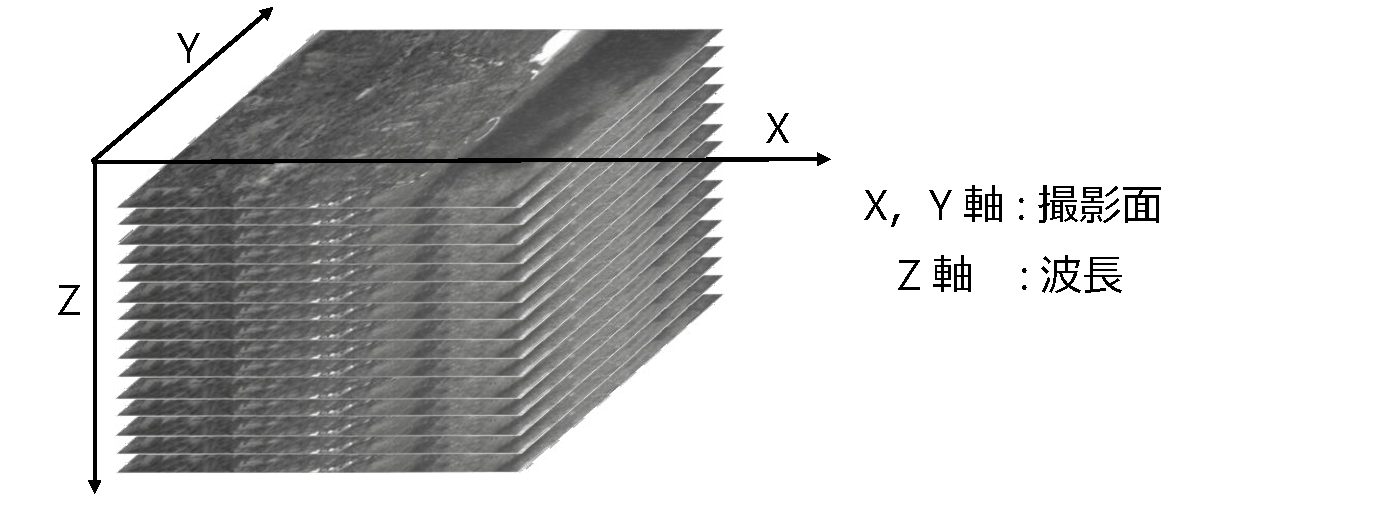
\includegraphics[width=11cm]{./Ch2_PrinciplesOfMethod/Fig/spectralimage_compressed.pdf}
% 	\caption{スペクトル画像}\label{fig:spectral_image}
% 	\end{center}
% \end{figure}

\begin{figure}[p]
	\begin{center}

		% \begin{minipage}[b]{0.9\linewidth}
		% \centering
		% 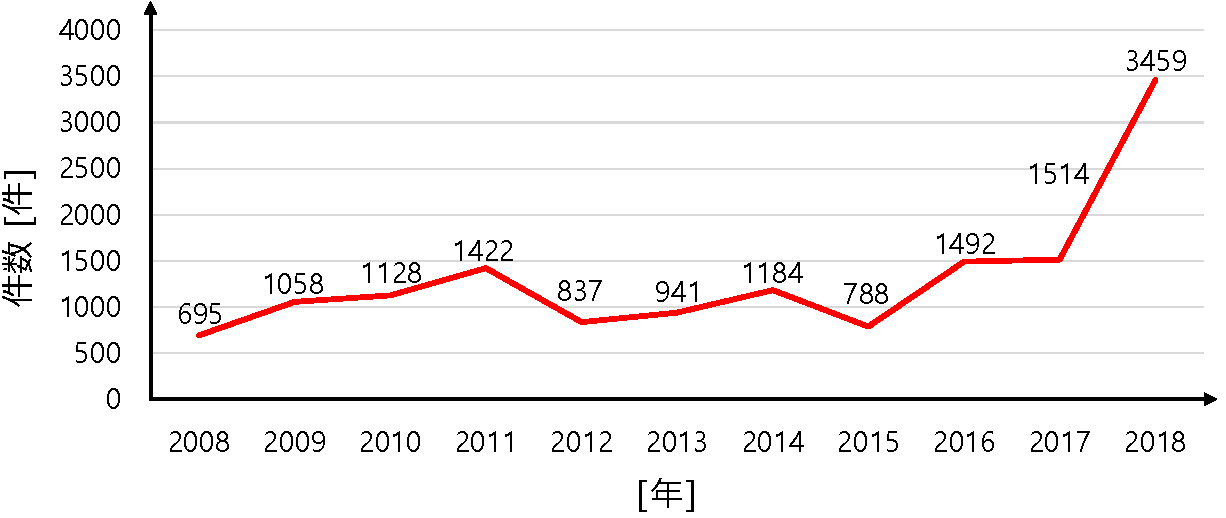
\includegraphics[width=12cm]{./Ch1_Introduction/Ch1_Fig/土砂災害発生件数.pdf}
		% \vspace{-3mm}
		% \caption*{(a)土砂災害発生件数}
		% \end{minipage}\\

		\begin{minipage}[b]{\linewidth}
		\centering
		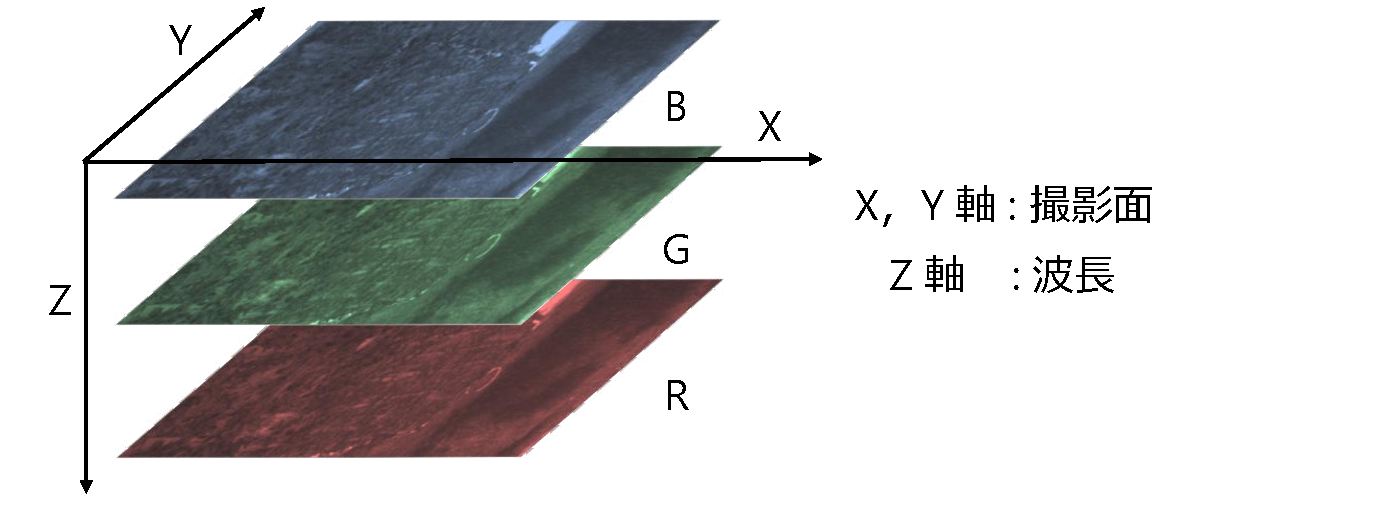
\includegraphics[width=12.5cm]{./Ch2_PrinciplesOfMethod/Fig/RGBimage_compressed.pdf}
		\vspace{-2mm}
		\caption*{(a)一般的なRGB画像} 
		\vspace{1cm} % 上下の画像の間を調整
		\end{minipage}\\

		\begin{minipage}[b]{\linewidth}
		\centering
		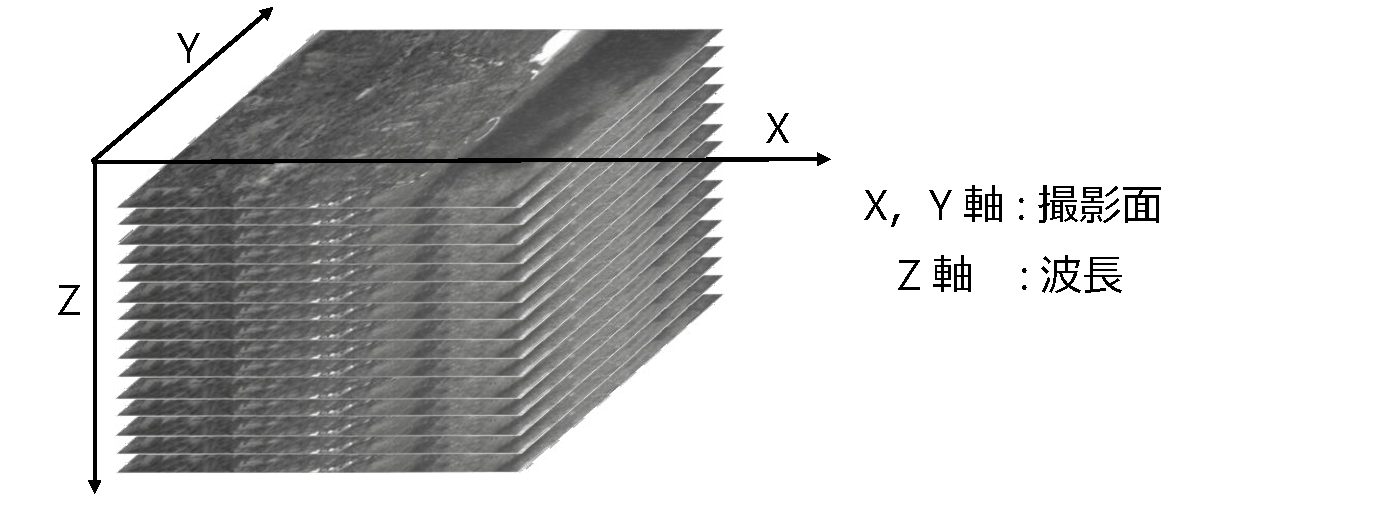
\includegraphics[width=12.5cm]{./Ch2_PrinciplesOfMethod/Fig/spectralimage_compressed.pdf}
		\vspace{-2mm}
		\caption*{(b)スペクトル画像} 
		\end{minipage}
	
	\caption{一般的なRGB画像とスペクトル画像の比較}\label{fig:RGBimage_spectralimage_comparison}
	\end{center}
\end{figure}

% ハイパースペクトル画像・マルチスペクトル画像は具体的な方法 
% スペクトル画像全般は原理で説明

\clearpage

\subsection{分光反射率スペクトルの取得}
\label{ssec:SpectrumGet}

スペクトル画像は,波長帯ごとの分光反射率が分かっている物質を画像に入れるように撮影することで,画像に写りこんだその物質以外の物質の
各波長帯における分光反射率を算出することができる.
その各波長帯の分光反射率を波長順に並べることによって,画像中の物質の分光反射率スペクトルを取得することができる.% 引用

そこで,本研究では,
% 従って,
分光反射率が既知の校正用物質を含めて撮影したスペクトル画像から
スペクトル画像内に分布している校正用物質以外の分光反射率スペクトルを取得する.
% 本研究ではこのようにしてスペクトル画像から分光反射率スペクトルを取得する.

% 土の分光反射率スペクトルの例を示す

\clearpage

\section{本研究で対象とする地盤}
\label{sec:Ground}

スペクトル画像を用いて土を撮影し,
土の種類の識別と含水比の推定を
行う場合,土の表面のみの情報からコーン指数を推定することになる.
従って,スペクトル画像
を用いてコーン指数を推定する場合,
従来のコーンペネトロメータを用いた手法で利用してきた
土の深い部分の情報を利用することができず,
表面の土のコーン指数のみを推定することになる.
しかし,一般的に,土は深いところにあるほど上の土の質量が増加するため
圧密により固くなる
ことが多い\cite{森本1975}\cite{高田1983}.
また,同じ場所ならば,基本的には表面にある土も深いところにある土も同じ種類の土である.
土の種類が同じならば圧密による固さの度合いは上に積層した土の質量のみに依存するため,
深いところにある土ほど固くなる.
災害現場の土も,上記で述べたような一般的にみられる土と同じ性質を持つと考えられる.
% 従って,スペクトル画像を用いた
そこで,本研究では,災害現場の土も上記で述べたような一般的にみられる土と同じ性質を持つと仮定して走破性判定を行う.
% 土の表面と深部における土の種類が同じであり,
% 深くなるにつれて土の硬さが単調に増加する地盤を対象とした走破性判定を行う.

以上の仮定に基づいて,スペクトル画像を用いて推定したコーン指数に基づく走破性判定を行った場合,
コーン指数の推定精度は土の深い部分の情報を利用できるコーンペネトロメータを用いた手法に劣るが,
一番上にある一番軟らかい土のコーン指数が建設機械の重量に耐えられるならば,
深い部分にある固い土のコーン指数も当然建設機械の重量に耐えるため,
建設機械の走破性判定を行うには十分であると考えられる.
従って,スペクトル画像を用いることによって,広範囲に対して一度に,簡易的かつ有効な走破性判定を行うことが期待できる.
% \begin{figure}[b]
% 	\begin{center}
% 	\centering
% 	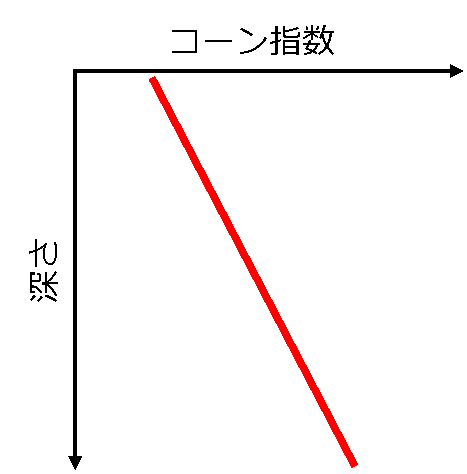
\includegraphics[width=4.5cm]{./Ch2_PrinciplesOfMethod/Fig/relationship_between_coneindex_and_depth_compressed.pdf}
% 	\caption{コーン指数と土の深さの関係}\label{fig:relationship_between_coneindex_and_depth}
% 	\end{center}
% \end{figure}

% 以上より,一番上にある一番軟らかい土のコーン指数が建設機械の重量に耐えられるならば,
% % 深い部分にある固い土のコーン指数も当然建設機械の重量に耐えるため,
% 土の表面にある一番軟らかい土の情報のみを利用して推定したコーン指数を用いた
% 非接触での走破性判定は有効である.



\clearpage

\section{土の種類の識別と含水比の推定に使用するスペクトル画像}
\label{sec:HyperAndMultiImages}

本研究では,スペクトル画像を用いて土の種類の識別と含水比の推定を行う.
具体的には,土の種類の識別と含水比の推定を行う際に,一般的なRGB画像が取得するR,G,Bの3波長帯以外の波長帯も取得するマルチスペクトル画像というスペクトル画像を用いる\cite{中野1996}.
% 具体的には,土の種類の識別には,波長幅の短い波長帯を多数取得できるハイパースペクトル画像を用い,
% 含水比の推定には,含水比の増加に伴って分光反射率が減少する近赤外の光を1つの波長帯で取得できる
% マルチスペクトル画像を用いる.

土の種類の識別の際には,水分子が吸収しない波長における分光反射率スペクトルの詳細な形状が必要になる.
そこで,入射光を分光して記録する波長帯の数が非常に多いマルチスペクトル画像を用いる.
% ハイパースペクトル画像とは,
% スペクトル画像の中でも,入射光を分光して記録する波長帯の数が非常に多いスペクトル画像である\cite{横矢2014}.
% 土の種類の識別の際には,水分子が吸収しない波長における分光反射率スペクトルの詳細な形状が必要になるため,
% そこで,入射光を分光して記録する波長帯の数が非常に多いマルチスペクトル画像を用いる.
% そこで,ハイパースペクトル画像を用いる.
% ハイパースペクトル画像とは,
マルチスペクトル画像を用いた土の種類の識別の詳細については,第\ref{ch:SoilTypeDiscrimination}章で解説する.
なお,このような,入射光を分光して記録する波長帯の数が非常に多いマルチスペクトル画像のことを,
マルチスペクトル画像の中でも特にハイパースペクトル画像という\cite{横矢2014}.

% 一方,マルチスペクトル画像とは,スペクトル画像のなかでも分光させる波長帯の数が少ない画像である.
一方,近赤外の光の分光反射率を用いて含水比を推定するためには,
近赤外の幅広い範囲の光を1つの波長帯として取得する分光反射率スペクトルを用いる必要がある.
そのため,含水比の推定の際には,%スペクトル画像のなかでも,
入射光を分光させる波長帯の数が少なく,1つの波長帯当たりの波長の幅を広く取ることが
できるマルチスペクトル画像を用いる.
マルチスペクトル画像を用いた含水比の推定の詳細については,第\ref{ch:WaterContentEstimation}章で解説する.

\clearpage

%==============================================================================
%おわりに
%==============================================================================
\section{おわりに}

本章では,スペクトル画像を用いて土の種類と含水比を推定し,その2つからコーン指数を推定する手法の原理について述べた.

まず,\ref{sec:PrimciplesOfConeindexEstimation}節において,
% 土の基礎的な性質を示す土質パラメータ
土の種類と含水比からコーン指数を推定する手法の原理の詳細について述べた.% "建設機械の走破性"
コーン指数は,土の基礎的な性質を示す土の粒子の鉱物組成,有機物含有量,粒度分布,球形率,含水比に大きく影響される.
本研究ではこれを利用し,外部の状況に左右されない,土に固有の土質パラメータである土の粒子の鉱物組成,有機物含有量,粒度分布,球形率
をひとまとめにした土の種類と,それに該当せず外部の状況によって変化する含水比の2つからコーン指数を推定する.

次に,\ref{sec:SpectrumAndMaterialRelationship}節において,
分光反射率スペクトルを用いて土の種類の識別と含水比の推定を行う手法の原理について述べた.
分光反射率スペクトルは物質の種類と状態によって変化するため,
物質の種類と状態を分光反射率スペクトルを用いて推定することが可能である.
そこで,本研究でも,分光反射率スペクトルを用いることによって,
土の種類の識別と含水比の推定を非接触に行う.
分光反射率スペクトルを用いて識別した土の種類と推定した含水比を用いてコーン指数を推定することによって,
非接触での建設機械の走破性判定を行う.

次に,\ref{sec:SpectrumFromSpectralImage}節において,
分光反射率スペクトルを取得するためのスペクトル画像について述べた.
建設機械の走破性を判定するためには,建設機械の走行面積以上の
広さのコーン指数を推定する必要があるため,広い面積の土の種類と含水比を
推定する必要があり,その範囲における分光反射率スペクトルを取得する必要がある.
従って,本研究では,
広い面積の分光反射率スペクトルを取得できるスペクトル画像を用いる.

また,\ref{sec:Ground}節において,
本研究で対象とする一般的な地盤について解説した後,
画像を用いて非接触での走破性判定を行うにあたり,
土の表面の情報のみを利用することについての議論を行った.
その議論において,本研究で対象とする一般的な地盤においては,
画像を用いて土の表面の情報のみを利用しても,
走破性の判定は
可能であることを示した.

最後に,\ref{sec:HyperAndMultiImages}節において,
本研究において,土の種類の識別と含水比の推定に用いるマルチスペクトル画像の違いと
それぞれの画像を使い分けた理由を簡単に解説した.

\newpage
%==============================================================================

\chapter{マルチスペクトル画像を用いた土の種類の識別}
\thispagestyle{empty}
\label{ch:SoilTypeDiscrimination}
\minitoc

\newpage
%%%%%%%%%%%%%%%%%%%%%%%%%%%%%%%%%%%%%%%%%%%%%%%%%%%%%%%%%%%%%%%%%%%%%%%%%%%%%%%
%==============================================================================
%はじめに
%==============================================================================
\section{はじめに}
本章では,非接触での走破性判定のために本研究で提案した,スペクトル画像を用いたコーン指数推定の最初のステップである,
スペクトル画像を用いた土の種類の識別の詳細について述べる.
本研究の提案手法において,本章で解説する部分を図\ref{fig:thesis_constitution_ch3}に茶色で示す.

% 本章では,スペクトル画像を用いて土の種類を識別する手法について述べる.
% 本研究では,土の種類を識別するため,スペクトル画像の中でも分光させる波長の数が多い
% ハイパースペクトル画像を使用する.

まず,\ref{sec:SoilTypeDiscriminationFromSpectrum}節において,
異なる土の種類がそれぞれ別の分光反射率スペクトルを持つことを利用して,
分光反射率スペクトルを用いて
土の種類の識別を非接触に行う手法について述べる.
% 分光反射率スペクトルを
% そして,分光反射率スペクトルを用いて土の種類を識別するためには,
% 詳細な分光反射率スペクトルの形状を知る必要性を述べる
なお,分光反射率スペクトルを用いて土の種類を識別するためには,
幅の狭い多数の波長帯の光の強さを記録する分光反射率スペクトルが
必要となるため,
波長分解能の高い分光反射率スペクトルを取得する必要があることを述べる.
% 波長幅の短い多数の波長帯から分光反射率を取得する必要があることを述べる.

次に,\ref{sec:ClassificationOfHyperspectralImage}節において,
土の種類を識別するための波長分解能の高い分光反射率スペクトルを取得するため,
スペクトル画像のなかでも分光させる波長帯の数が非常に多いマルチスペクトル画像を用いることを述べる.
% ハイパースペクトル画像を用いた土の種類の識別について述べる.

最後に,\ref{sec:PreliminaryExperimentOfDiscrimination}節において,
\ref{sec:SoilTypeDiscriminationFromSpectrum}節と\ref{sec:ClassificationOfHyperspectralImage}節で解説した手法の
有効性を確認するために行った,マルチスペクトル画像を用いて土の種類を識別する検証実験について述べる.

\begin{figure}[p]
	\begin{center}
	\centering
	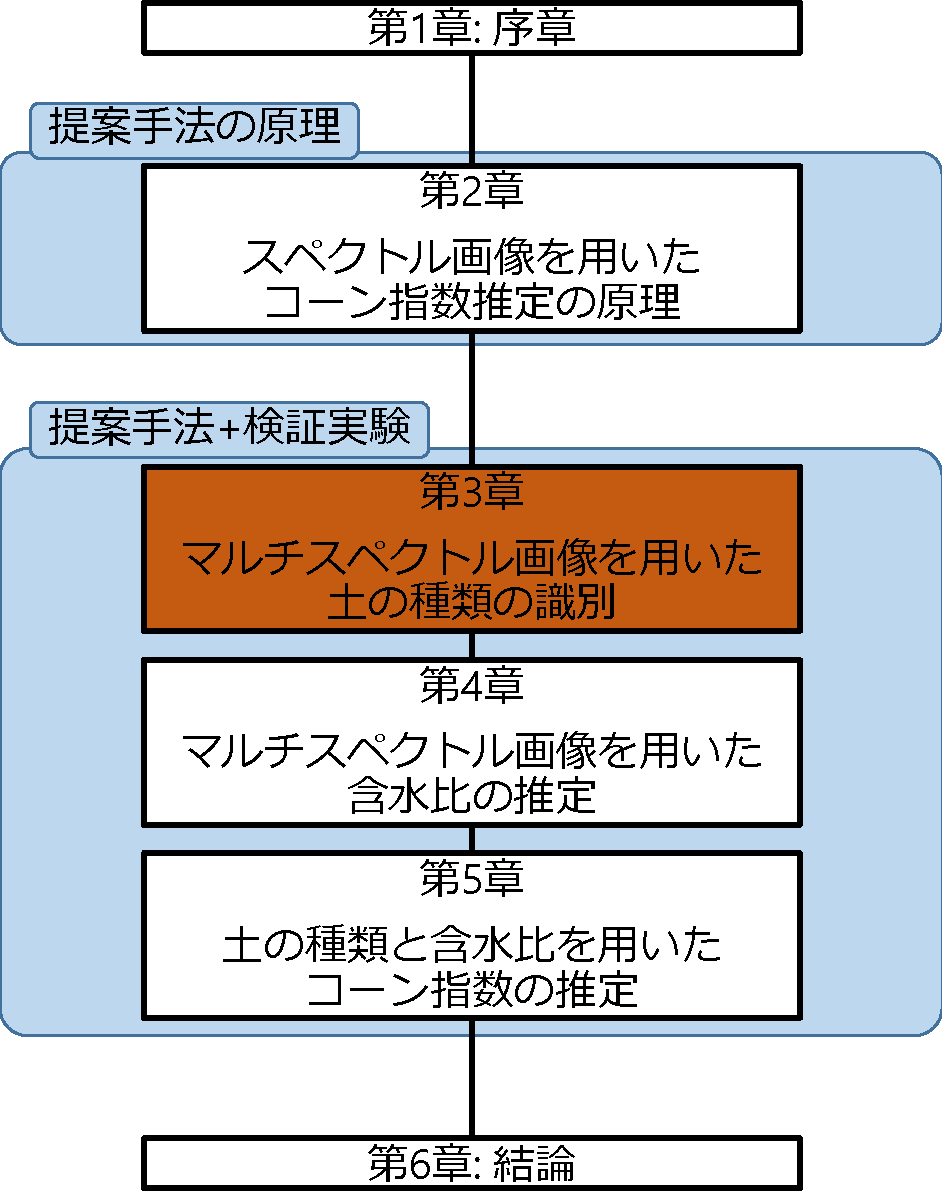
\includegraphics[width=8cm]{./Ch3_SoilTypeDiscrimination/Fig/thesis_constitution_ch3_compressed.pdf}
	\caption{本章で解説する部分(茶色の部分)}\label{fig:thesis_constitution_ch3}
	\end{center}
\end{figure}


\clearpage


%==============================================================================
%分光反射率スペクトルを用いた土の種類の識別
%==============================================================================
\section{分光反射率スペクトルを用いた土の種類の識別}
\label{sec:SoilTypeDiscriminationFromSpectrum}

\ref{sec:PrimciplesOfConeindexEstimation}節で述べた通り,
土の基本的な性質を示す土質パラメータはコーン指数に大きく影響する.
そこで,本研究では,
様々な土のうち,
% コーン指数に大きく影響する,土の基本的な性質を示す
土の基本的な性質を示す土質パラメータの中でも
外部の状況に左右されない,土に固有の土質パラメータである,土の粒子の鉱物組成,有機物含有量,粒度分布,球形率が同じ土を
同じ種類の土と定義した.
従って,土の種類が異なると,これらの外部の状況に左右されない土に固有の土質パラメータも異なることになる.

また,\ref{sec:SpectrumAndMaterialRelationship}節で述べた通り,
物質は,その分子や原子の構造,または物質を構成する微粒子の大きさや形,表面の凹凸によって,
光の波長ごとの反射,散乱,吸収,そして放射の度合いが異なるため,
物質の種類と状態が異なると分光反射率スペクトルも異なる.
従って,土の種類が異なると土の粒子の材質や直径の分布,形,表面の粗さも異なるため,
土の種類ごとに異なる分光反射率スペクトルを持つ.
本研究ではこれを利用して,
予め土の種類ごとに測定した分光反射率スペクトル
を用いて土の種類を識別する.

土の種類ごとに異なる分光反射率スペクトルを持つ例を図\ref{fig:spectrum_for_different_soiltype}に示す.
図\ref{fig:spectrum_for_different_soiltype}に示したグラフにおいて,縦軸は分光反射率,横軸は波長を示す.
また,グラフ中の黒,赤,青の3本の曲線は,それぞれ異なる土の種類である,粘性土,火山灰質粘性土,礫質土の分光反射率スペクトルを示す.
この3種類の土の種類は,異なる場所で採取された異なる種類の土である.
このうち,粘性土と火山灰質粘性土は,共に,0.075mm未満の,粘土と呼ばれる土の粒子が最も大きな割合を占める土である.
一方,礫質土は,2mmから75mmまでの,礫と呼ばれる土の粒子が最も大きな割合を占める土である.% 引用
上記の3種類の土の画像を図\ref{fig:different_soiltype_image}に示す.

\begin{figure}[p]
	\begin{center}
		\begin{tabular}{c}

			\begin{minipage}[t]{\linewidth}
			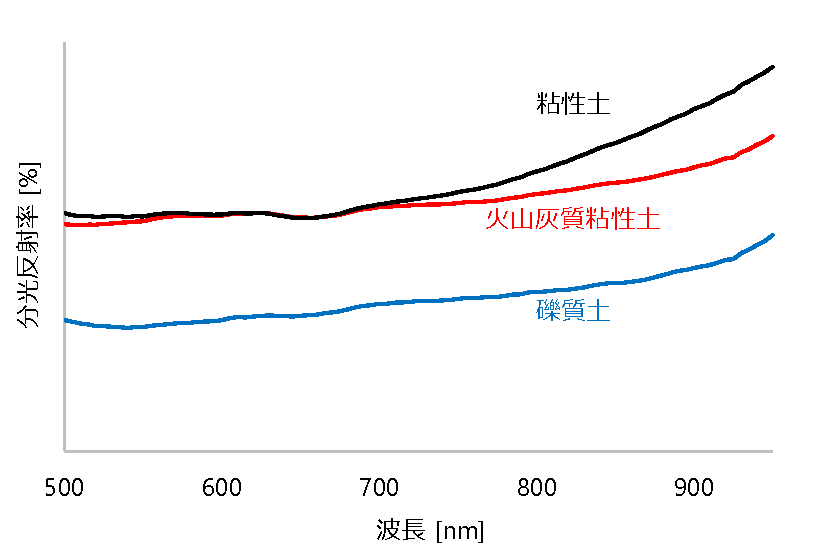
\includegraphics[width=13cm]{./Ch3_SoilTypeDiscrimination/Fig/spectrum_for_different_soiltype_compressed.pdf}
			\caption{土の種類ごとに異なる分光反射率スペクトル}\label{fig:spectrum_for_different_soiltype}
			\vspace{2cm}
			\end{minipage}

			\\

			\begin{minipage}[t]{0.33\linewidth}
			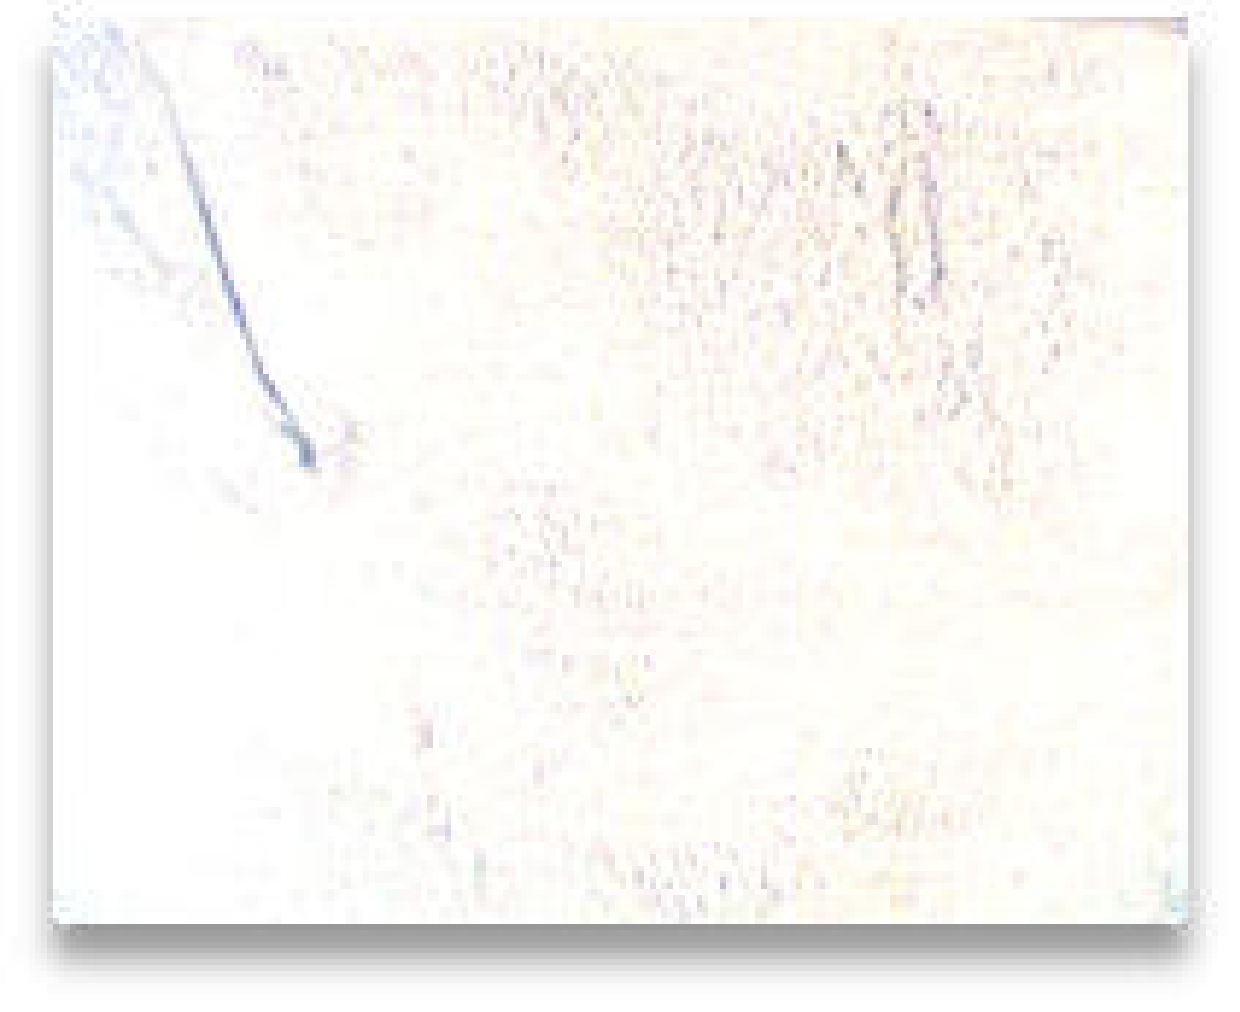
\includegraphics[width=4cm]{./Ch3_SoilTypeDiscrimination/Fig/A_Fu_image_compressed.pdf}
			\caption*{粘性土}
			\end{minipage}

			\hfill

			\begin{minipage}[t]{0.33\linewidth}
			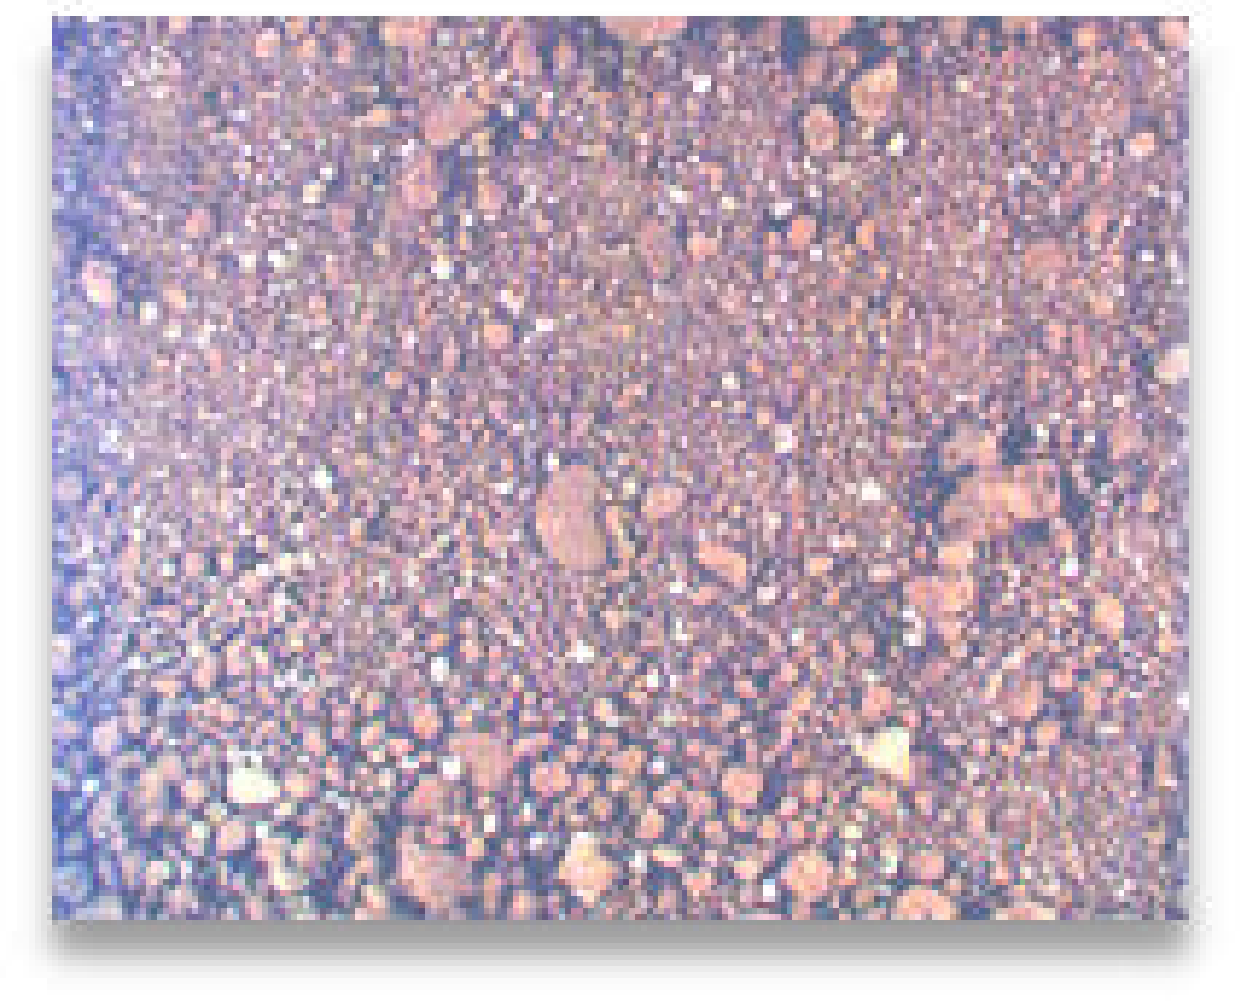
\includegraphics[width=4cm]{./Ch3_SoilTypeDiscrimination/Fig/B_Is_image_compressed.pdf}
			\caption*{火山灰質粘性土}
			\end{minipage}

			\hfill

			\begin{minipage}[t]{0.33\linewidth}
			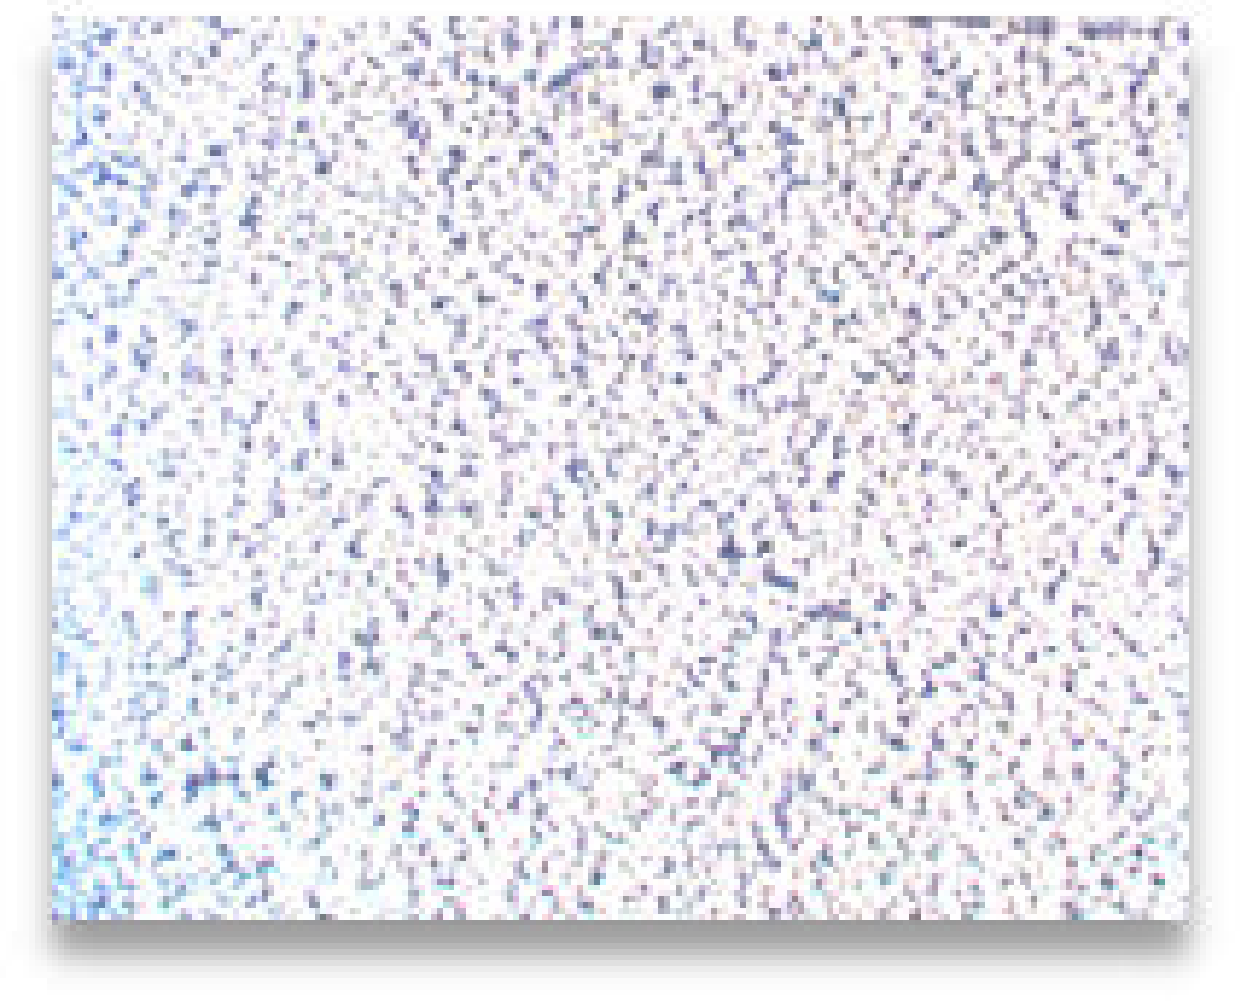
\includegraphics[width=4cm]{./Ch3_SoilTypeDiscrimination/Fig/C_K1_image_compressed.pdf}
			\caption*{礫質土}
			\end{minipage}

		\end{tabular}
		\caption{分光反射率スペクトルを比較した3種類の異なる土の画像}\label{fig:different_soiltype_image}
	\end{center}
\end{figure}

\clearpage

図\ref{fig:spectrum_for_different_soiltype}より,
土の種類ごとに異なる分光反射率スペクトルが存在することが分かる.
% ここにもう1つ項(土の種類の識別に必要な分光反射率スペクトルの要件)を入れて,波長分解能についてより詳しく述べる
% なぜ高い波長分解能が必要なのか
% 1つの節に1つの項だけでは不自然
しかし,多くの種類の土を分光反射率スペクトルで識別するためには,
図\ref{fig:spectrum_for_different_soiltype}に示したような,非常に多くの波長帯の光の強さを記録する
% 波長分解能の高い why
分光反射率スペクトル
を知る必要がある.
6種類の土を本研究と同様の手法で,取得する波長帯の数が異なる画像から識別した際の識別精度を図\ref{fig:discrimination_accuracy_by_wavelength_number}に示す.図\ref{fig:discrimination_accuracy_by_wavelength_number}において,縦軸は土の種類の識別精度,
横軸は各画像で取得する波長帯の数を示す.
図\ref{fig:discrimination_accuracy_by_wavelength_number}より,
波長帯の数が多くなる程,画像を用いた土の種類の識別精度が向上することが分かる.

非常に多くの波長帯の光の強さを記録する
分光反射率スペクトルを取得するためには,入射光を幅の短い多数の波長帯に分光させる,
波長分解能の高いスペクトル画像を用いる必要がある.
そのために,本研究では,スペクトル画像の中でも,波長分解能の高い
マルチスペクトル画像を使用する.
この波長分解能の高いマルチスペクトル画像を用いて,非常に多くの波長帯の光の強さを記録する分光反射率スペクトル
を取得し,土の種類の識別に利用する.

\begin{figure}[b]
	\begin{center}
	\centering
	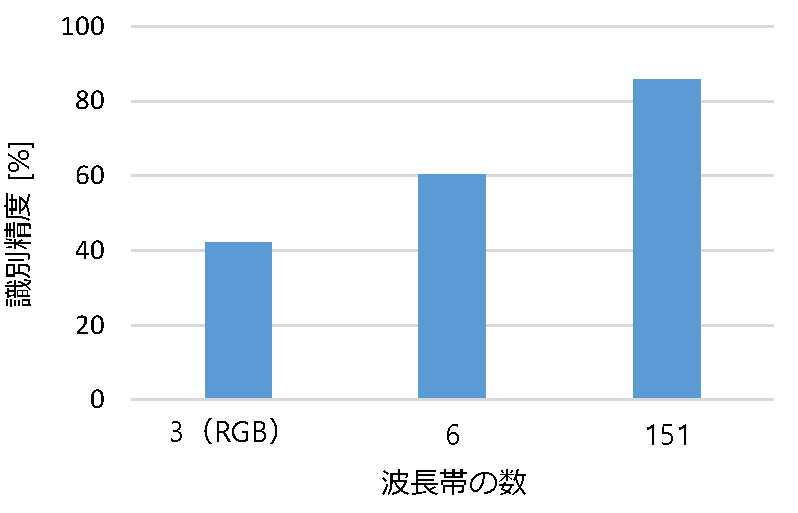
\includegraphics[width=10cm]{./Ch3_SoilTypeDiscrimination/Fig/discrimination_accuracy_by_wavelength_number_compressed.pdf}
	\caption{取得する波長帯の数が異なる画像を用いた土の種類の識別精度の比較}\label{fig:discrimination_accuracy_by_wavelength_number}
	\vspace{1cm}
	\end{center}
\end{figure}

\clearpage


\section{マルチスペクトル画像の分類}
\label{sec:ClassificationOfHyperspectralImage}

\subsection{波長帯の数が非常に多いマルチスペクトル画像}
\label{ssec:HyperspectralImage}

マルチスペクトル画像とは,
スペクトル画像の中でも,一般的なRGB画像が取得するR,G,Bの3波長帯以外の波長帯も取得するマルチスペクトル画像というスペクトル画像を用いる\cite{中野1996}.

本研究において土の種類の識別に用いるマルチスペクトル画像は,
対象とする物体を走査するように撮影するため,
マルチスペクトル画像を構成する画素ごと,あるいは画素の列ごとに% "ピクセル"にすると目立つので,"画素"で統一
入射光を分光させて得た分光反射率スペクトルを記録し,
それを終えると,次の画素や画素の列の
入射光を分光して分光反射率スペクトルを記録し始める.
そのため,
画素ごとに,撮影時にその画素内に映し出された物質の分光反射率スペクトルが記録されている.
従って,マルチスペクトル画像から分光反射率スペクトルを取得するには,
画素ごとに取得する.

また,\ref{sec:HyperAndMultiImages}節で述べた,本研究でも使用するような,
入射光を分光して記録する波長帯の数が非常に多いマルチスペクトル画像は
1980年代に衛星に搭載されるようになり,
広範囲に渡る地表の鉱物資源の分布の調査,植生の分布の調査,生態系の監視などに使用されている\cite{Underwood2003}\cite{Kruse2003}\cite{Ustin2004}\cite{Haboudane2004}\cite{Clark2005}.

\clearpage

\subsection{ニューラルネットワークによる分類}
\label{ssec:NeuralNetWork}

\ref{ssec:HyperspectralImage}項において述べた通り,
本研究では,マルチスペクトル画像から取得した分光反射率スペクトルを用いて土の種類を識別する.
分光反射率スペクトルは非線形であり,また他の物質からの光の散乱によって本来の形状を乱されることも多いので,
ニューラルネットワークを用いて識別を行う.
分光反射率スペクトルを用いて土の種類を識別するために,
分光反射率スペクトルを示すベクトルを入力層とし,出力層のノードの数を識別する土の種類の数,
中間層を入力層の約半分の数のノードで構成した,3層のニューラルネットワークを用いる.
まず,マルチスペクトル画像から画素ごとに記録されている分光反射率スペクトルを取得し,
取得した分光反射率スペクトルがホワイトアウトまたはブラックアウトしていないかどうかを確認して,
ニューラルネットワークに入力する.
なお,ホワイトアウトもブラックアウトもしていない分光反射率スペクトルの数が100以下のマルチスペクトル画像は
土の種類の識別には使用しないこととする.
ホワイトアウトもブラックアウトもしていない分光反射率スペクトルの数が100より多いマルチスペクトル画像から
取得した分光反射率スペクトルに土の種類のラベルを付け,土の種類の識別を行う.
分光反射率スペクトルはマルチスペクトル画像が取得する波長帯の数の成分を持つベクトルとして存在し,
それぞれの成分は0以上1未満となる.
分光反射率スペクトルを示す,マルチスペクトル画像が取得する波長帯の数の成分を持つベクトルを,
そのままニューラルネットワークの入力層として使用する.
本研究で使用するニューラルネットワークは,3層の全結合層から構成されている.
上記で解説した入力層と全結合する中間層は,入力層の約半分の数のノードで構成されており,
活性化関数にはReLUを使用する.
中間層と全結合する出力層は,識別する土の種類の数と同じ数のノードで構成されており,
活性化関数にはSoftmaxを使用する.
中間層と出力層の間ではドロップアウトを行い,ドロップアウトする割合は0.2に設定する.
このニューラルネットワークの最適化にはRMSporpを使用し,学習率は0.001に設定する.

マルチスペクトル画像から画素ごとに記録されている分光反射率スペクトルを取得し,
ニューラルネットワークを用いて土の種類を識別する様子を,
図\ref{fig:neuralnetwork}に示す.
図\ref{fig:neuralnetwork}において,
左側にあるのがマルチスペクトル画像であり,
右側にあるのが本研究で使用したニューラルネットワークである.
また,マルチスペクトル画像の上にある赤いひし形は1つの画素を示しており,
各画素ごとに記録された分光反射率スペクトルを取得して,
それをニューラルネットワークに入力する様子を示している.

図\ref{fig:neuralnetwork}に示すニューラルネットワークにおいて,
本研究では入力層のノードの数$C_r$が151,中間層のノードの数$m$が65となる.
また,出力層のノードの数$n$は,この後の\ref{sec:PreliminaryExperimentOfDiscrimination}節で述べる
マルチスペクトル画像から土の種類を識別する検証実験ではその検証実験で識別する土の種類の数である10となり,
\ref{sec:ConeindexEstimationExperiment}節で述べる,
コーン指数の推定の検証実験ではその検証実験で識別する土の種類の数である6となる.

\begin{figure}[b]
	\begin{center}
	\centering
	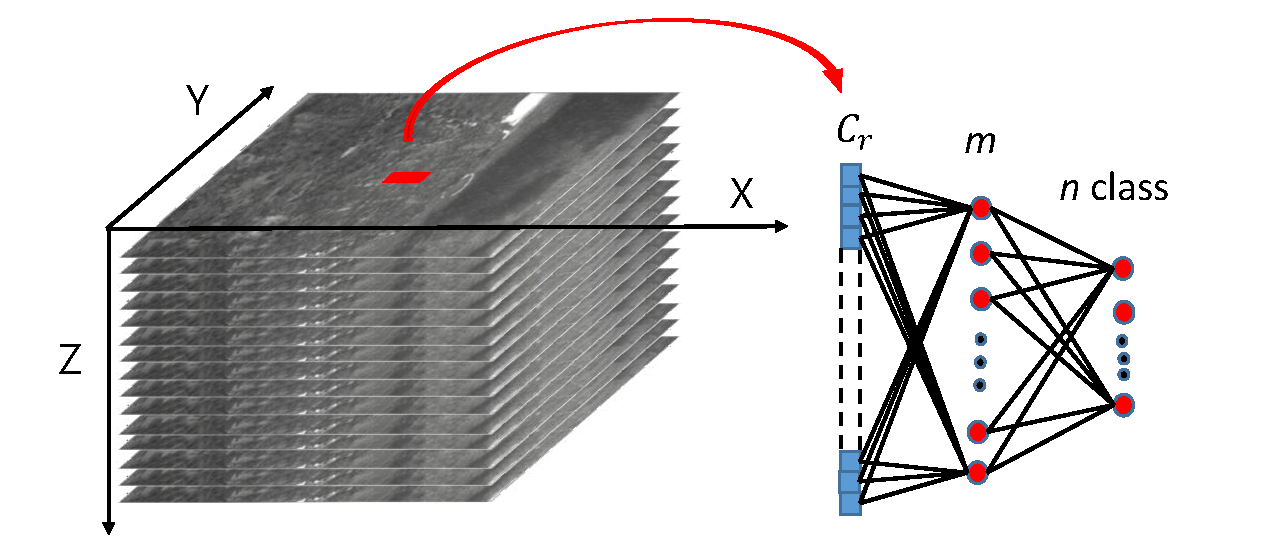
\includegraphics[width=13cm]{./Ch3_SoilTypeDiscrimination/Fig/neuralnetwork_for_hyperspectralimage_compressed.pdf}
	\caption{マルチスペクトル画像を分類するニューラルネットワーク}\label{fig:neuralnetwork}
	\vspace{6cm}
	\end{center}
\end{figure}

\clearpage

%==============================================================================
%土の種類を識別する検証実験
%==============================================================================
\section{土の種類を識別する検証実験}
\label{sec:PreliminaryExperimentOfDiscrimination}

\ref{sec:SoilTypeDiscriminationFromSpectrum}節と\ref{sec:ClassificationOfHyperspectralImage}節で
解説した,マルチスペクトル画像から取得した分光反射率スペクトルを用いた土の種類の識別の有効性を確認するため,
検証実験を行った.
% また,本研究において土の種類の識別に使用するマルチスペクトル画像は,入射光を分光して記録する波長帯の数が非常に多いため,
% \ref{sec:HyperAndMultiImages}節で述べたように,\ref{sec:PreliminaryExperimentOfDiscrimination}節で使用する,
% 取得する波長帯の数が非常に多いマルチスペクトル画像のことをハイパースペクトル画像と呼称する.

\subsection{実験環境}
\label{ssec:DiscriminationExperimentSetting}

今回の検証実験の目的は,
土の種類の違いによる分光反射率スペクトルの違いから,土の種類の識別を行うことができるか確認することである.
そのため,土の種類の違い以外の要因による分光反射率スペクトルの変動をなるべく除外する必要がある.
本研究の目的は,災害現場における建設機械の非接触での走破性判定である.
従って,マルチスペクトル画像の撮影時には屋外で太陽光を光源とする.
しかし,太陽光は時間や天候などの条件によって光量が変動するため,
屋外で同じ物質をマルチスペクトル画像で撮影しても,撮影時の環境の条件によって
取得した分光反射率スペクトルが変動する可能性がある.
% 従って,今回の検証実験において,太陽光を光源として使用することは困難である.
そこで,太陽光に似たスペクトルを持っているハロゲンランプを光源としてマルチスペクトル画像を
撮影することにした.
これにより,環境の条件の変化による土の分光反射率スペクトルの変動を除外しつつ,
太陽光を光源とした場合と似た分光反射率スペクトルをマルチスペクトル画像から取得することができる.
今回の検証実験におけるマルチスペクトル画像の撮影時の撮影機材の配置を図\ref{fig:discrimination_experiment_setting}に示す.% 実験の概要は"様子",各種の数値で表現できる場合は"条件"とする
図\ref{fig:discrimination_experiment_setting}に示す通り,土を入れた容器を中心にして,周囲を囲むように3つのハロゲンランプを配置して,
マルチスペクトル画像の撮影に十分な光量を確保した.
そして,マルチスペクトル画像を撮影するためのマルチスペクトルカメラを,土を入れた容器の直上に配置して撮影を行った.
なお,今回の検証実験で使用したマルチスペクトルカメラは,エバ・ジャパン株式会社製のNH-7である.
NH-7の写真と具体的な仕様を,それぞれ図\ref{fig:hyperspectral_camera}と表\ref{tbl:hyperspectral_camera}に示す.
% また,NH-7の具体的な仕様を表\ref{tbl:hyperspectral_camera}に示す.
また,土の含水比を0$\%$に揃えて撮影を行った.

\begin{figure}[p]
	\begin{center}
		\begin{tabular}{c}

			\begin{minipage}[t]{\linewidth}
			\hspace{3cm}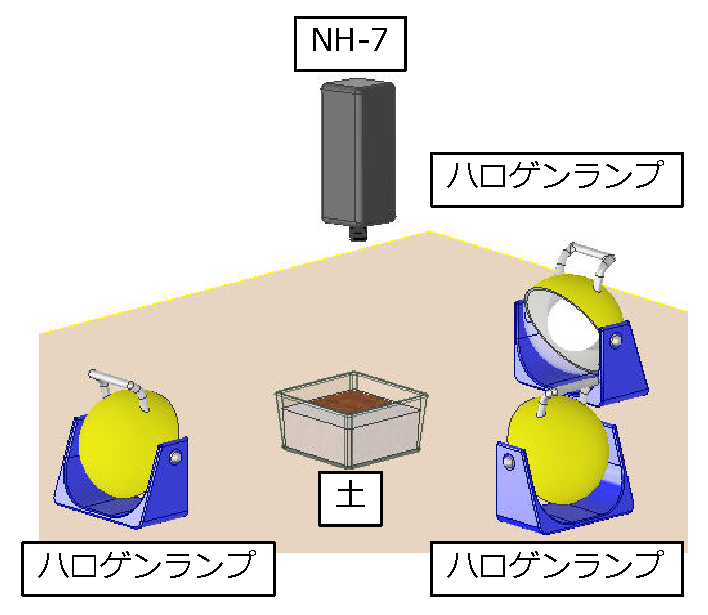
\includegraphics[width=7cm]{./Ch3_SoilTypeDiscrimination/Fig/discrimination_experiment_setting_compressed.pdf}
			\caption{検証実験における撮影機材の配置}\label{fig:discrimination_experiment_setting}
			\vspace{2cm}
			\end{minipage}

		\end{tabular}
	\end{center}
\end{figure}

\begin{figure}[b]
	\begin{center}
		\begin{tabular}{c}

			\begin{minipage}[b]{0.5\linewidth}
			% \vspace{1.5cm}
			% \hspace{4cm}
			\hspace{1cm}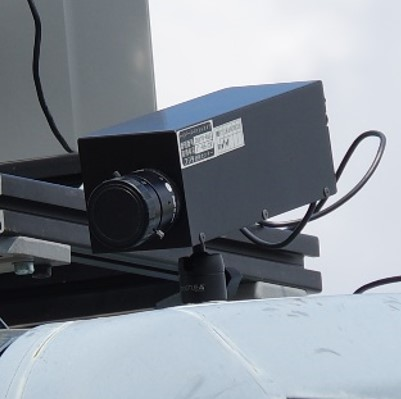
\includegraphics[width=5cm]{./Ch3_SoilTypeDiscrimination/Fig/hyperspectral_camera.jpg}
			\caption{NH-7}\label{fig:hyperspectral_camera}
			\vspace{1.5cm}
			\end{minipage}

			\hfill

			\begin{minipage}[b]{0.5\linewidth}
			\vspace{-2cm} % 表の高さを右のマルチスペクトルカメラの仕様を示した表と合わせる
			\tblcaption{NH-7の仕様}\label{tbl:hyperspectral_camera}
			
				\begin{center}
					% \hspace{4cm}
					\begin{tabular}{|c|c|} \hline
					製品名 & NH-7 \\ 
					(メーカー)& (エバジャパン)\\ \hline
					波長 & 350 $\sim$ 1100nm \\ 
					   &(ピッチ: 5nm)\\ \hline
					波長帯数 & 151 \\ \hline
					\end{tabular}
				\end{center}
			% \vspace{0.2cm} % 図表のタイトルを右と合わせる
			\vspace{3cm}
			\end{minipage}

		\end{tabular}
	\end{center}
\end{figure}

\clearpage

\subsection{実験データ}
\label{ssec:DiscriminationExperimentalProcedure}

今回の検証実験では,全国の異なる場所から集めた10種類の土を使用した.
集めた10種類の土のうち,5種類は,土を構成する土粒子のうち半分以上の直径が0.075mm以上75mm未満の粗粒土,
残りの5種類が,土を構成する土粒子のうち半分以上の直径が0.075mm未満の細粒土である.
また,5種類の細粒土は,さらにその土の起源によって,粘性土と火山灰質粘性土に分けられる.
今回使用した10種類の土のRGB画像を図\ref{fig:discrimination_experiment_data}に示す.
図\ref{fig:discrimination_experiment_data}のRGB画像の下には
,それぞれの土が粗粒土,粘性土,火山灰質粘性土のどれであるかを記載した.
また,この10種類を,表にある通り,以降AからJの名前で呼称する.

\begin{figure}[p]
	\begin{center}
		\begin{tabular}{c}

			\begin{minipage}[t]{0.33\linewidth}
			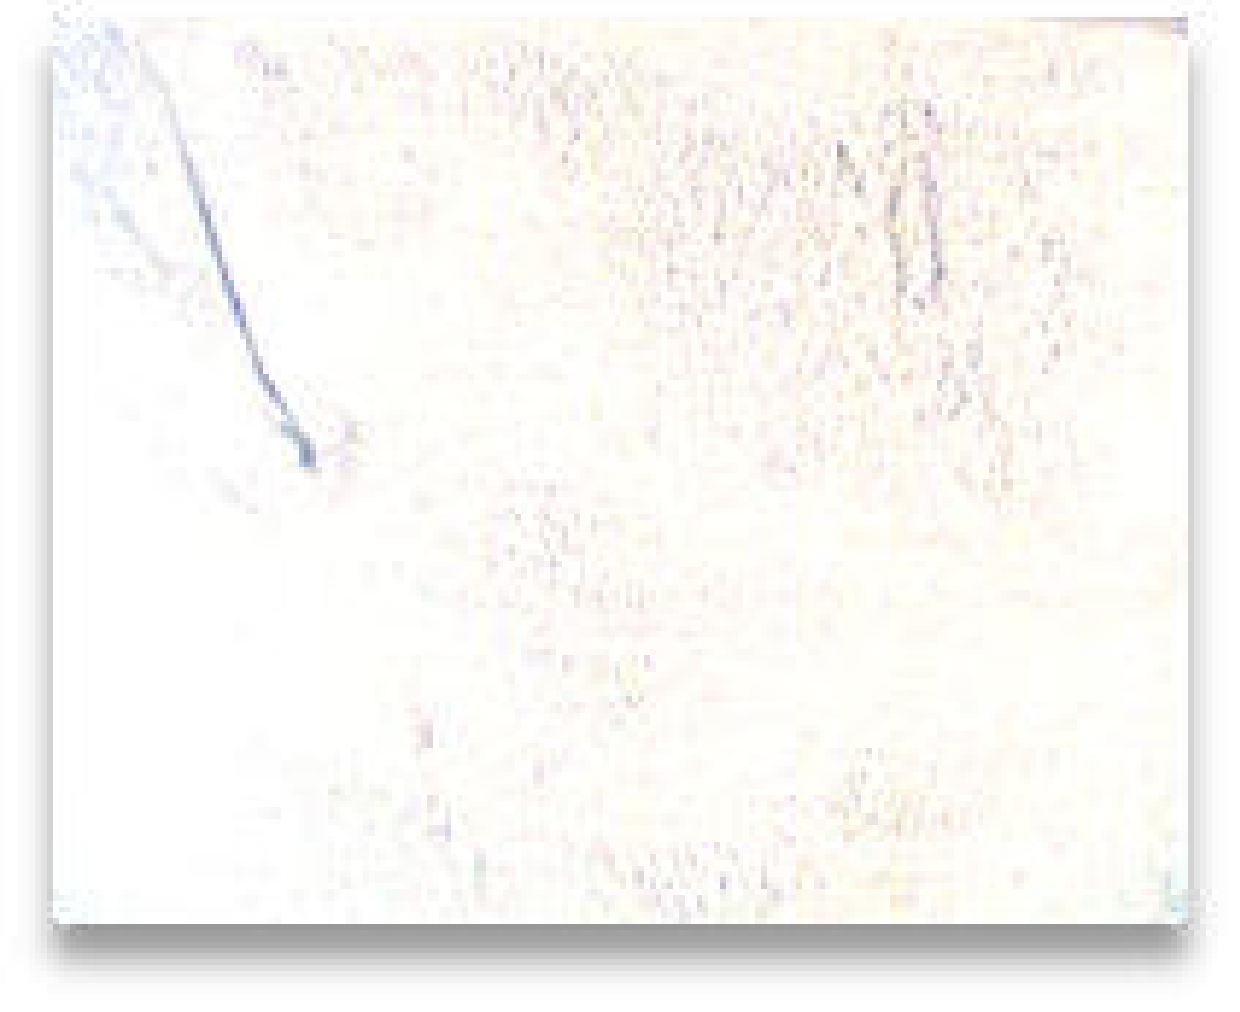
\includegraphics[width=4cm]{./Ch3_SoilTypeDiscrimination/Fig/A_Fu_image_compressed.pdf}
			\caption*{(a)土の種類A(粘性土)} % 京都府
			% \vspace{2cm}
			\end{minipage}

			\begin{minipage}[t]{0.33\linewidth}
			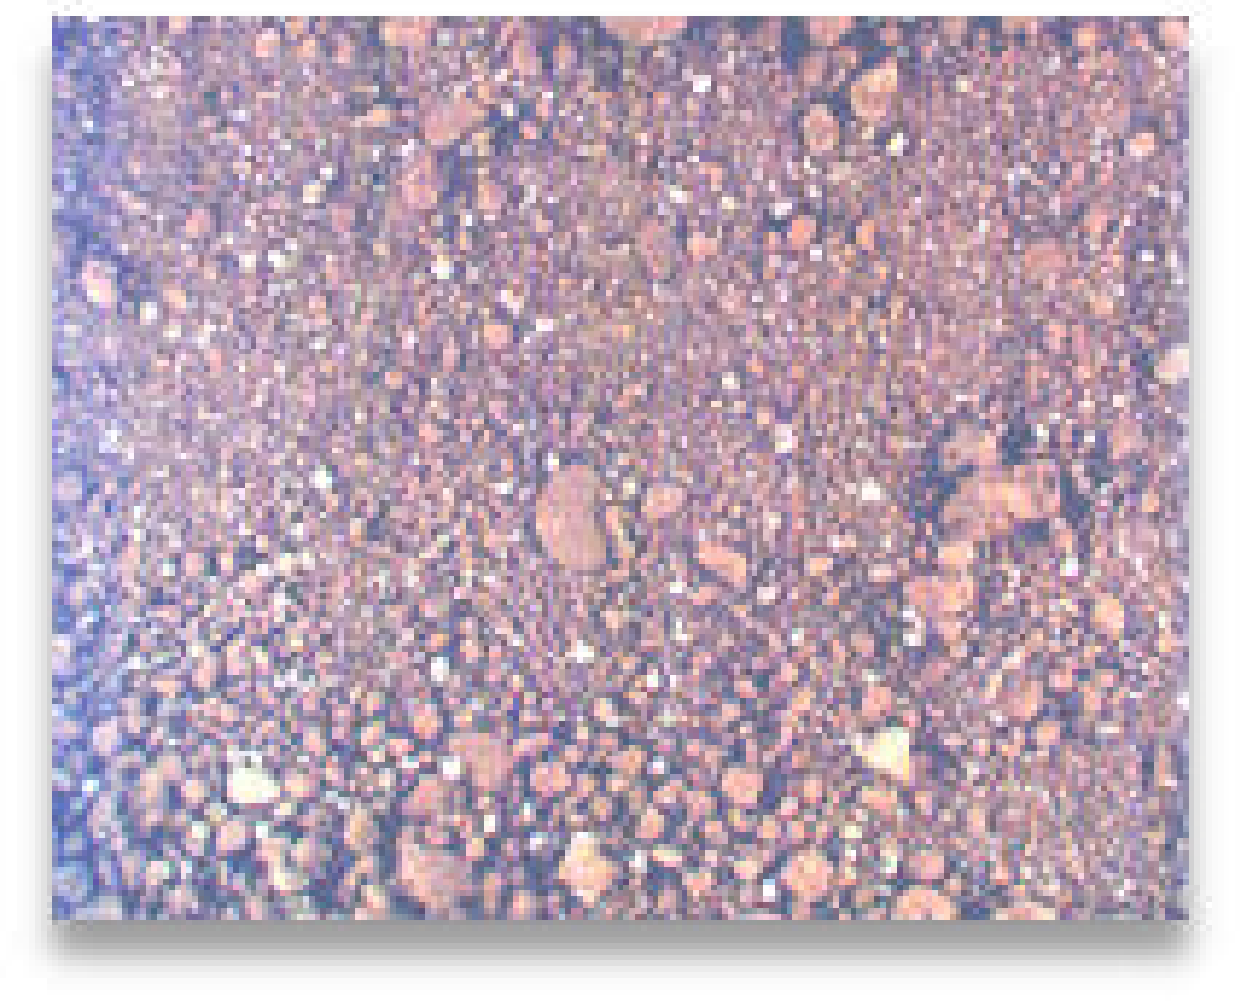
\includegraphics[width=4cm]{./Ch3_SoilTypeDiscrimination/Fig/B_Is_image_compressed.pdf}
			\caption*{(b)土の種類B(火山灰質粘性土)} % 神奈川県伊勢原市
			\end{minipage}

			\hfill

			\begin{minipage}[t]{0.33\linewidth}
			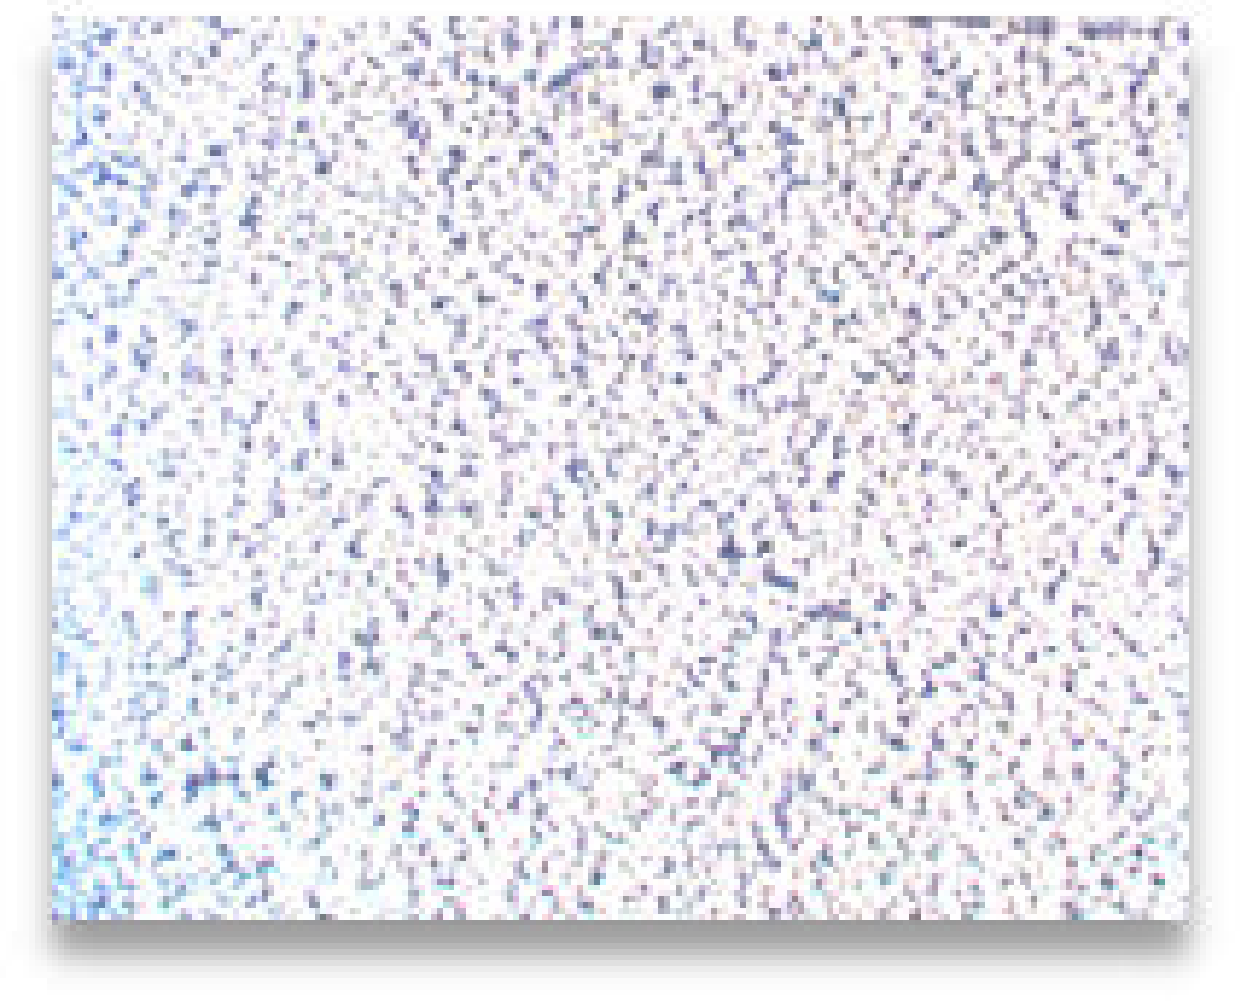
\includegraphics[width=4cm]{./Ch3_SoilTypeDiscrimination/Fig/C_K1_image_compressed.pdf}
			\caption*{(c)土の種類C(粗粒土)} % 硅砂1号
			\end{minipage}

			\\

			\begin{minipage}[t]{0.33\linewidth}
			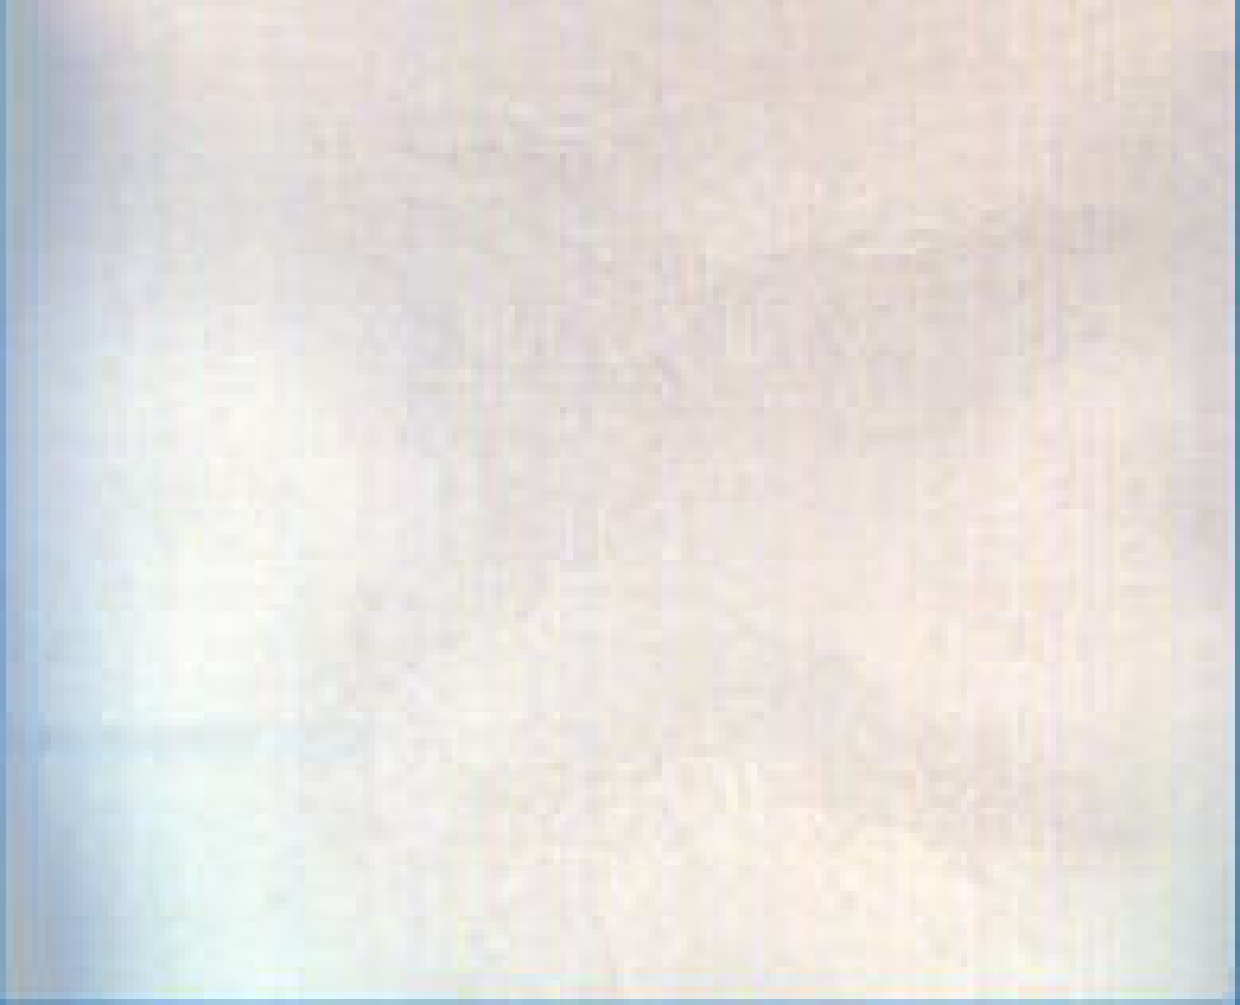
\includegraphics[width=4cm]{./Ch3_SoilTypeDiscrimination/Fig/D_K9_image_compressed.pdf}
			\caption*{(d)土の種類D(粘性土)} % 硅砂9号
			% \vspace{2cm}
			\end{minipage}

			\begin{minipage}[t]{0.33\linewidth}
			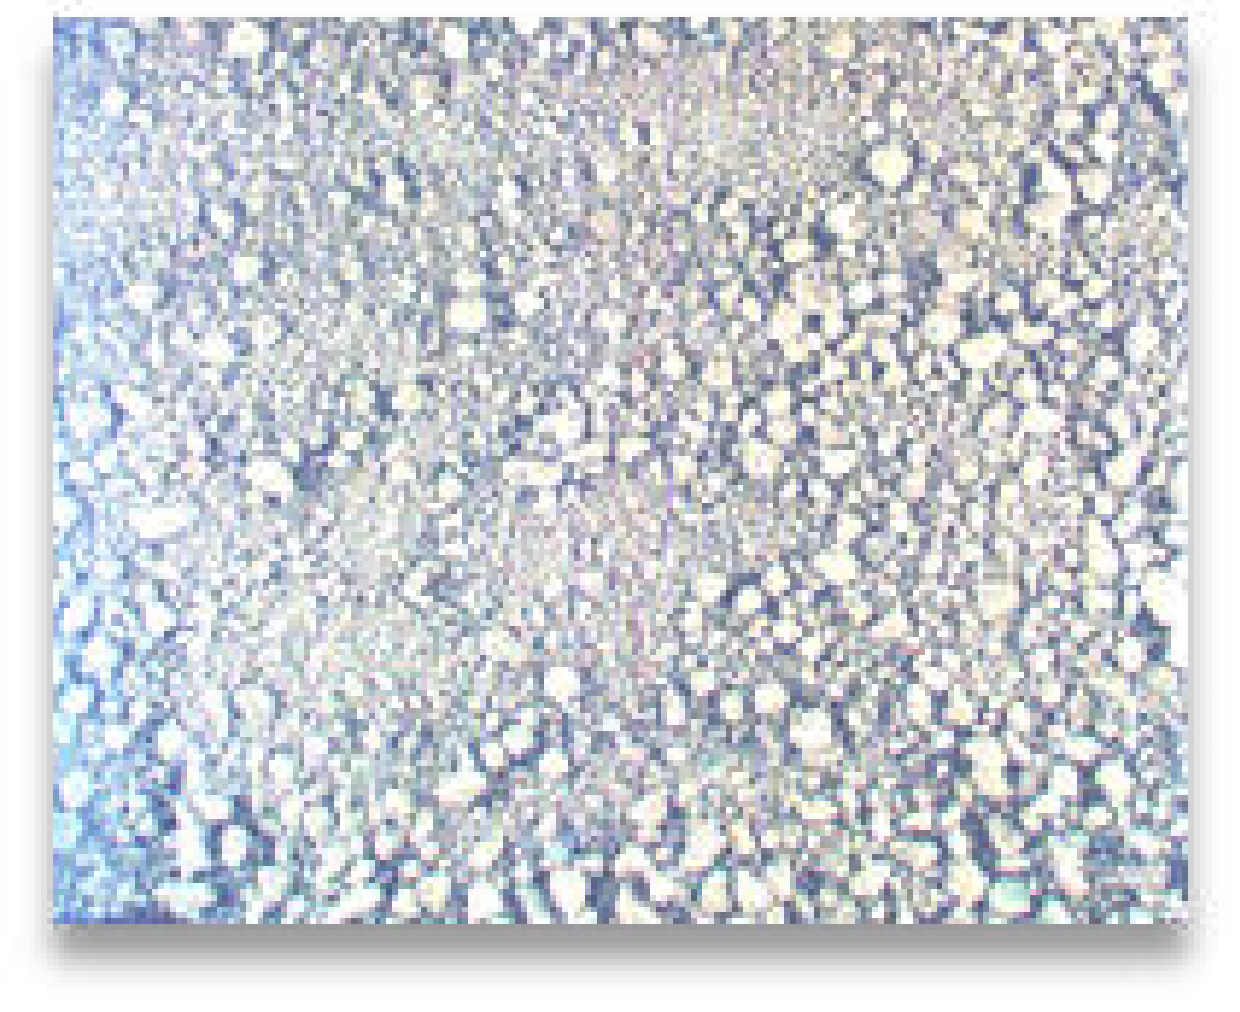
\includegraphics[width=4cm]{./Ch3_SoilTypeDiscrimination/Fig/E_Ko_image_compressed.pdf}
			\caption*{(e)土の種類E(粗粒土)} % 三重県三重郡
			\end{minipage}

			\hfill

			\begin{minipage}[t]{0.33\linewidth}
			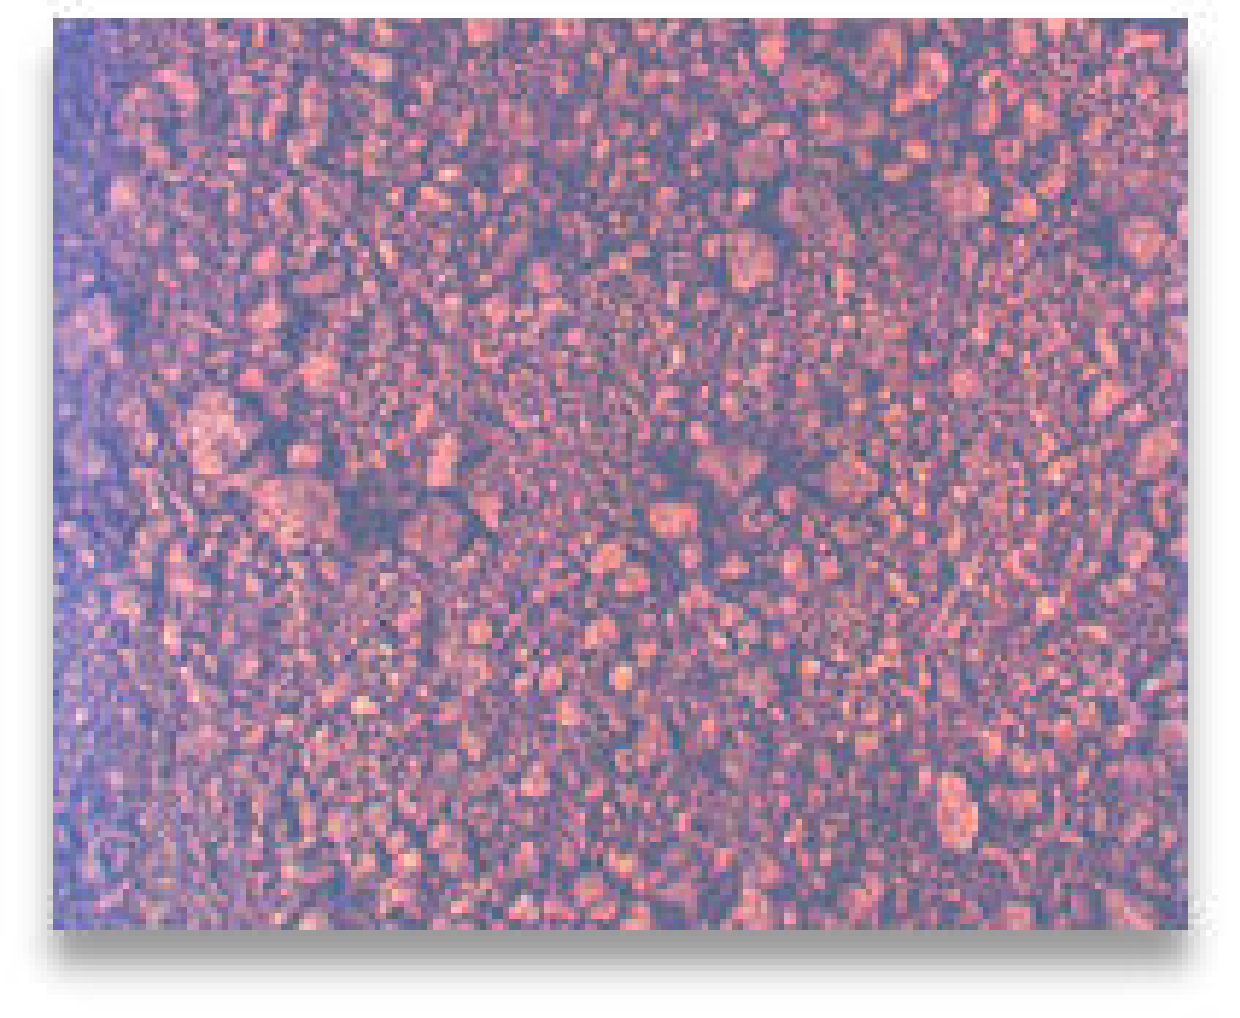
\includegraphics[width=4cm]{./Ch3_SoilTypeDiscrimination/Fig/F_Lo_image_compressed.pdf}
			\caption*{(f)土の種類F(火山灰質粘性土)} % 静岡県御殿場市
			\end{minipage}

			\\

			\begin{minipage}[t]{0.33\linewidth}
			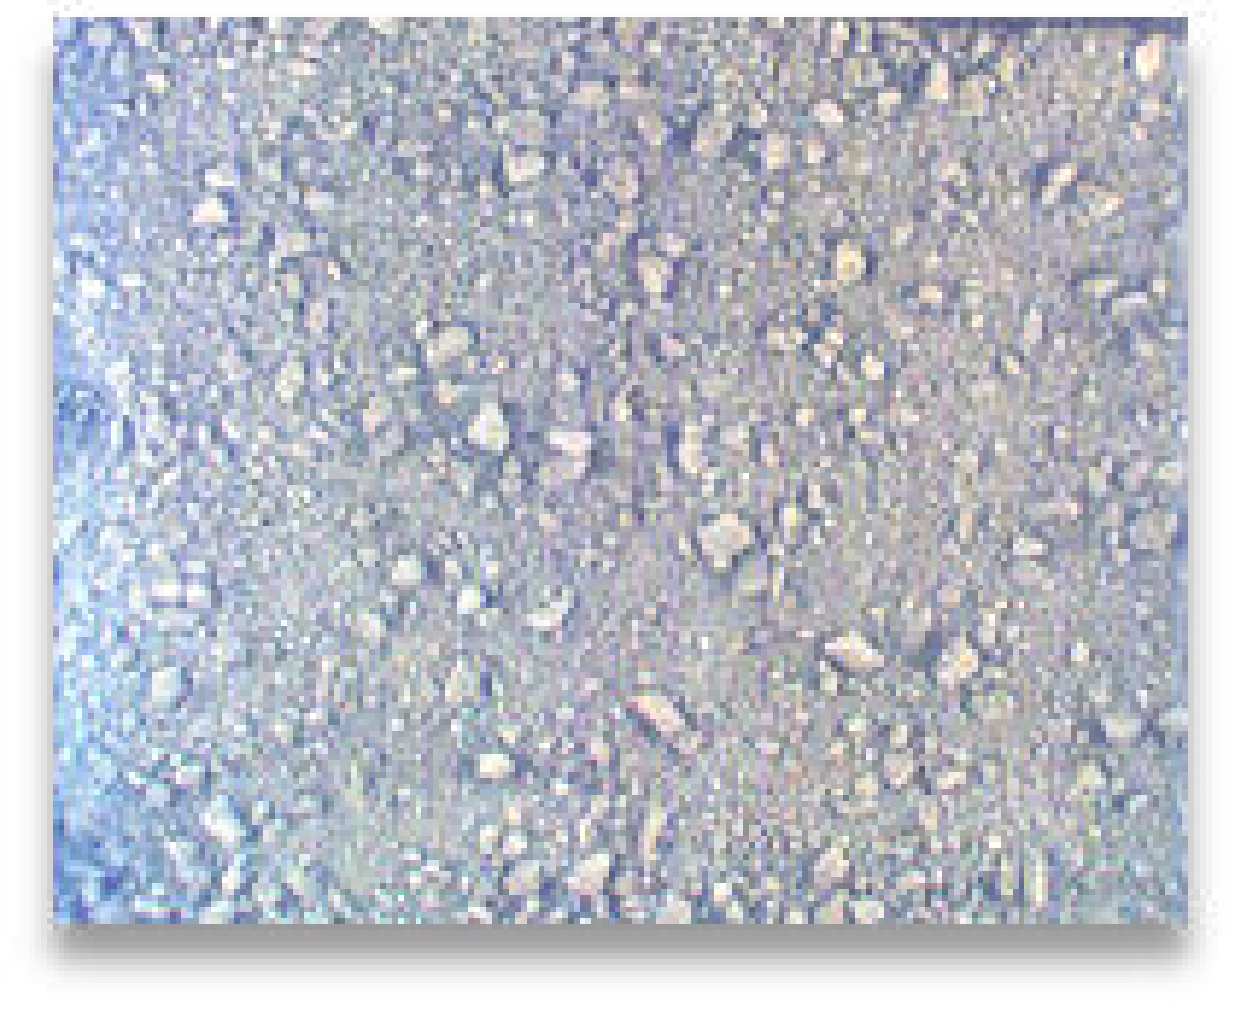
\includegraphics[width=4cm]{./Ch3_SoilTypeDiscrimination/Fig/G_Mi_image_compressed.pdf}
			\caption*{(g)土の種類G(粘性土)} % 宮崎県?
 			% \vspace{2cm}
			\end{minipage}

			\begin{minipage}[t]{0.33\linewidth}
			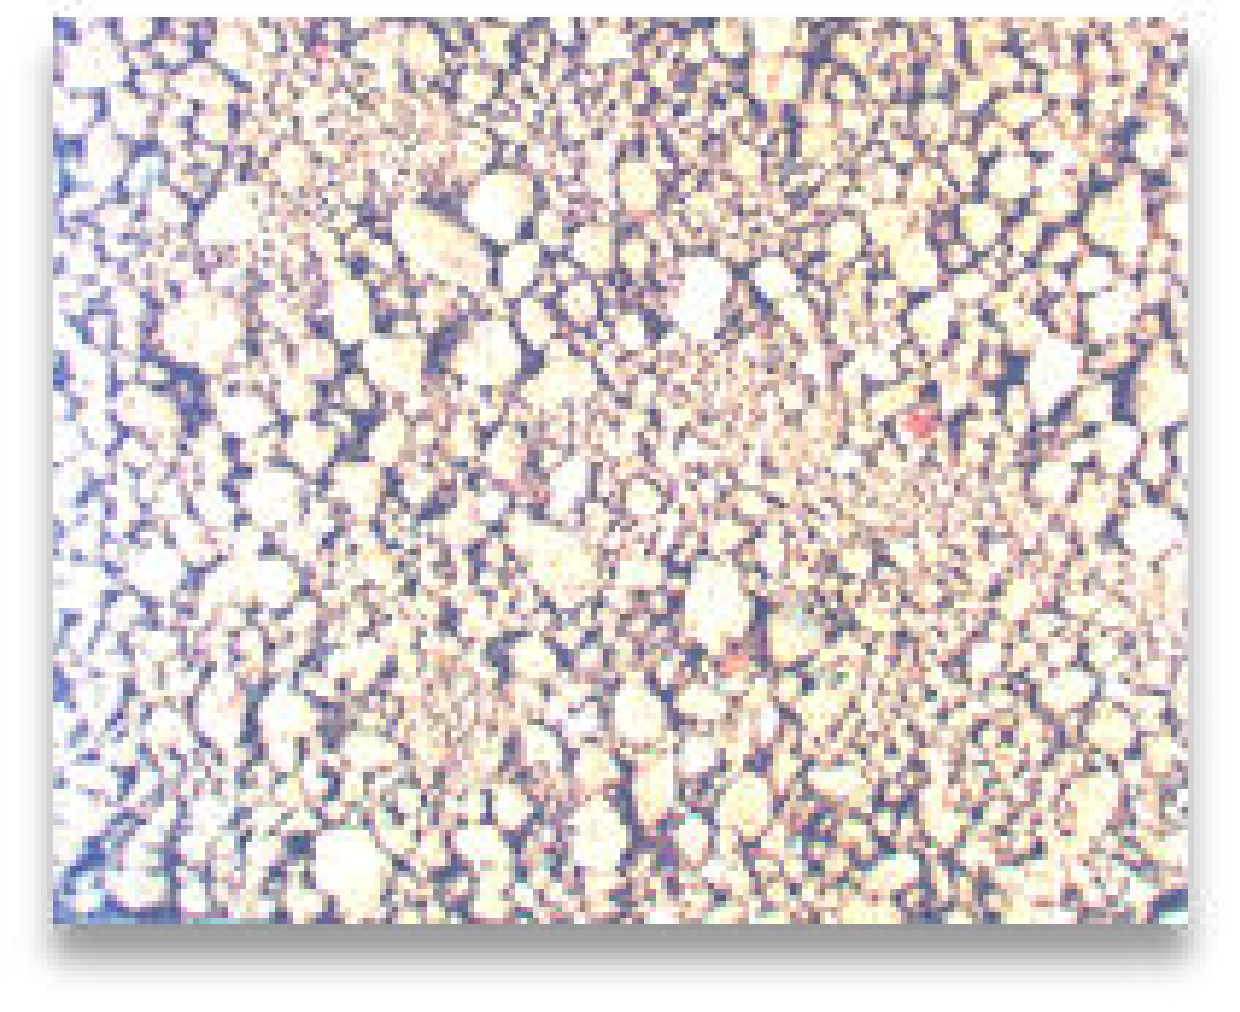
\includegraphics[width=4cm]{./Ch3_SoilTypeDiscrimination/Fig/H_Oh_image_compressed.pdf}
			\caption*{(h)土の種類H(粗粒土)} % 北海道?,青森県?,岩手県?
			\end{minipage}

			\hfill

			\begin{minipage}[t]{0.33\linewidth}
			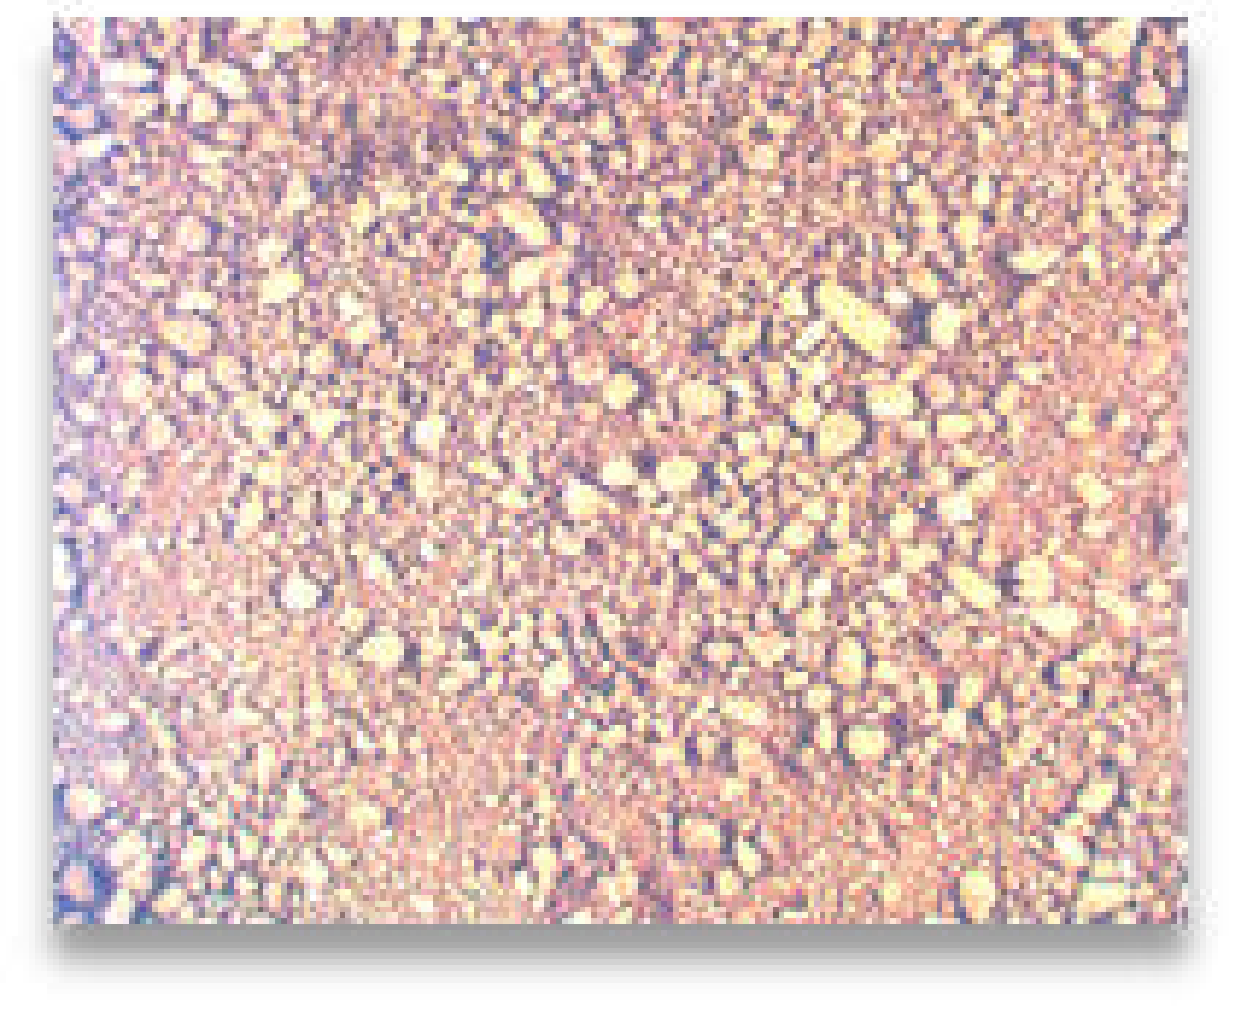
\includegraphics[width=4cm]{./Ch3_SoilTypeDiscrimination/Fig/I_Sa_image_compressed.pdf}
			\caption*{(i)土の種類I(粗粒土)} % 大阪府茨木市
			\end{minipage}

			\\

			\begin{minipage}[t]{0.33\linewidth}
			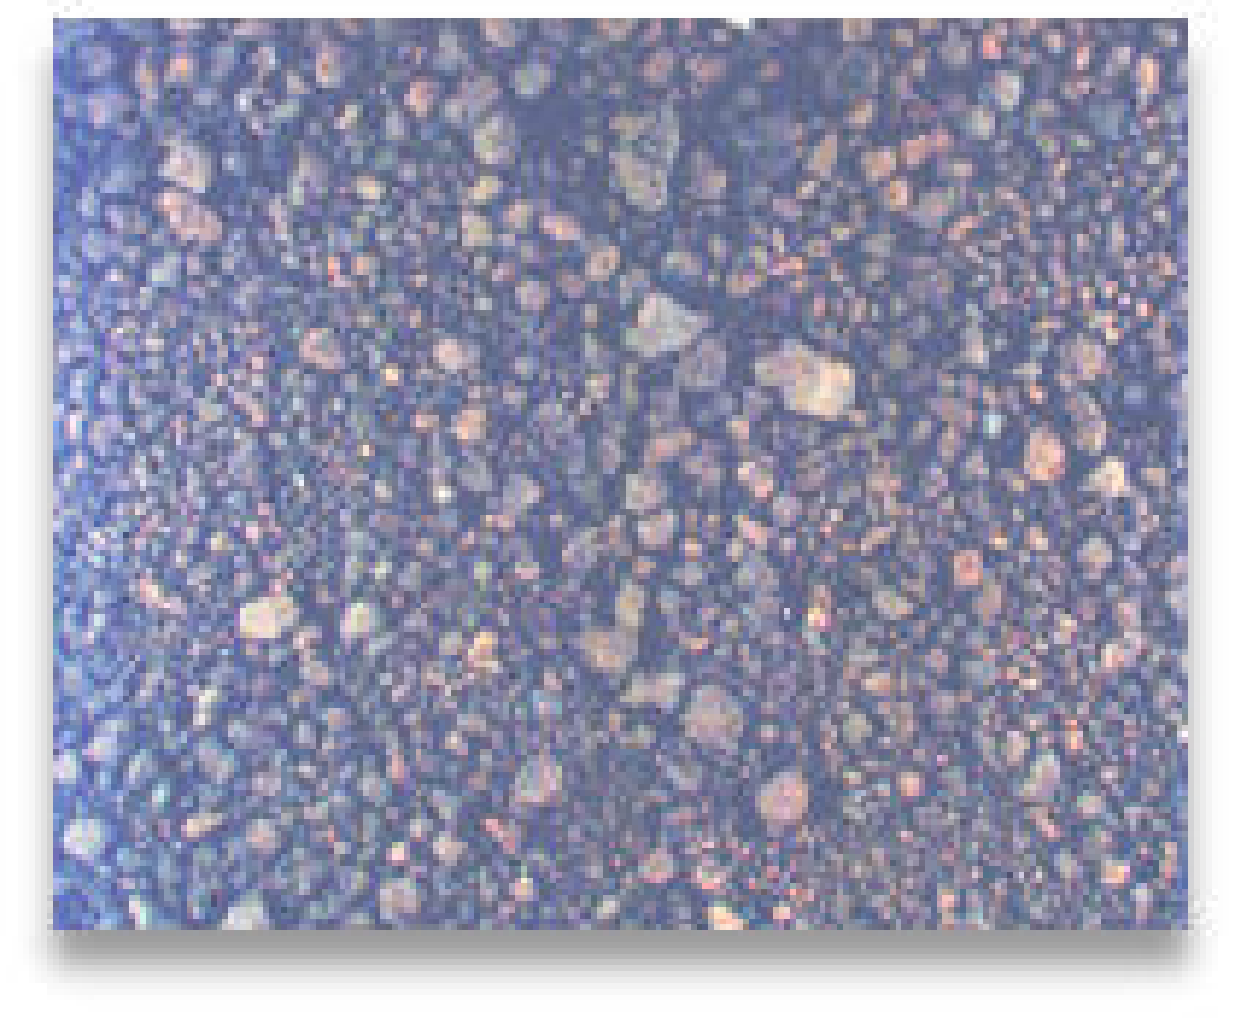
\includegraphics[width=4cm]{./Ch3_SoilTypeDiscrimination/Fig/J_Sc_image_compressed.pdf}
			\caption*{(j)土の種類J(粗粒土)} % 静岡県御殿場市
			\end{minipage}

		\end{tabular}
		\caption{土の種類を識別する検証実験用のデータ}\label{fig:discrimination_experiment_data}
	\end{center}
\end{figure}

\clearpage

\subsection{実験結果}
\label{ssec:DiscriminationResult}

\ref{ssec:NeuralNetWork}項で解説したニューラルネットワークを,
バッチサイズを128,エポック数を12に設定して学習を行った.
学習したニューラルネットワークを用いて,10種類の土を撮影したマルチスペクトル画像から取得した
分光反射率スペクトルを識別した結果の混同行列を
図\ref{fig:discrimination_confusion_matrix}に示す.
% このニューラルネットワークのトレーニングは,.
この混同行列は,縦軸がマルチスペクトル画像の各画素の分光反射率スペクトルの実際の土の種類を示し,
横軸がその分光反射率スペクトルをニューラルネットワークで識別した結果を示す.
各分光反射率スペクトルが撮影された実際の土の種類と,ニューラルネットワークによって識別された土の種類が一致した
場合は,混同行列の対角成分の部分の確率が高くなる.
この混同行列における確率は,高くなるほど濃い青色になる.
確率と色の濃さの対応を,図\ref{fig:discrimination_confusion_matrix}の右側にあるカラーバーに示す.
この混同行列から分かる通り,使用した10種類の土全てにおいて高い確率で
分光反射率スペクトルから実際の土の種類を識別できていることが分かる.
また,今回のニューラルネットワークによる土の種類の識別の結果,
全体の正解率が81.57\%となった.

\begin{figure}[b]
	\begin{center}
	\centering
	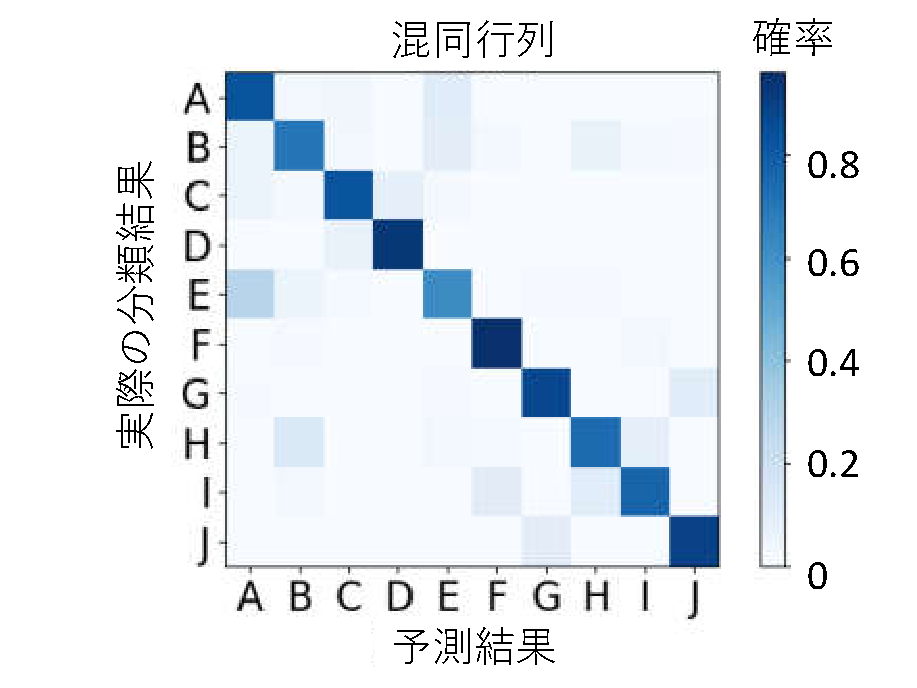
\includegraphics[width=8cm]{./Ch3_SoilTypeDiscrimination/Fig/confusion_matrix_compressed.pdf}
	\caption{10種類の土の識別結果を示す混同行列}\label{fig:discrimination_confusion_matrix}
	\end{center}
\end{figure}

\clearpage

\subsection{考察}
\label{ssec:DiscriminationConsideration}

今回の検証実験の結果より,マルチスペクトル画像から取得した分光反射率スペクトルを用いた土の種類の識別精度は
高いことが分かった.
従って,土の種類の違いによる分光反射率スペクトルの違いから,ニューラルネットワークを用いることによって
高い精度で土の種類を識別できることが確認出来た.
これは,マルチスペクトル画像から幅の狭い波長帯を数多く取得することによって
非常に多くの波長帯の光の強さを記録する分光反射率スペクトルを取得し,
1つの土の種類に対して十分詳細な分光反射率スペクトルの形状をニューラルネットワークに学習させることが
できたためである.
また,この\ref{sec:PreliminaryExperimentOfDiscrimination}節で解説した土の種類を識別する検証実験では,
マルチスペクトル画像を屋内の暗室でハロゲンランプを光源にして撮影したが,
\ref{ssec:DiscriminationExperimentSetting}項で述べた通り,
ハロゲンランプと太陽光は似たスペクトルを持つため,太陽光を光源にしても,
土の種類の違いによる分光反射率スペクトルの違いをニューラルネットワークによって捉え,
高精度で土の種類を識別することが期待できる.

% "詳細"と"詳細でない"の違いを明確にして

% 非常に多くの波長帯の光の強さを記録する
% % 波長分解能の高い why
% 分光反射率スペクトル

しかし,一部の土では少し推定精度が落ちることも分かった.
例えば,図\ref{fig:discrimination_confusion_matrix}の混同行列における各成分の確率より,
実際の種類はEである土がAであると識別されたり,実際の種類はHである土がBやIと識別される確率が
僅かに他の誤認識の場合に比べて高いことが分かる.
図\ref{fig:discrimination_experiment_data}において,
土の種類Eと土の種類A,あるいは土の種類H,土の種類B,および土の種類IのRGB画像を比較すると,
それぞれ土粒子の大きさが多少異なっているが,
EとAは共に白みががっており,H,B,およびIは共に赤みががっていることが分かる.
よって,似た色あいの土の種類は分光反射率スペクトルが似た形状になるため,
識別精度が落ちることが分かる.
本研究では,分光反射率スペクトルを用いて土の種類を識別するため,
土の粒子の材質に比べて粒度分布の情報を取得しにくいと考えられる.
このような誤認識を低減させるためには,
マルチスペクトル画像の画素ごとの分光反射率スペクトルのみを考慮するのではなく,
マルチスペクトル画像のテクスチャも考慮する必要がある.

\newpage


%==============================================================================
%おわりに
%==============================================================================
\section{おわりに}

本章では,非接触での走破性判定のために本研究で提案した,スペクトル画像を用いたコーン指数推定の最初のステップである,
マルチスペクトル画像から取得した分光反射率スペクトルを用いた土の種類の識別の詳細について述べた.

まず,\ref{sec:SoilTypeDiscriminationFromSpectrum}節において,
土の種類が異なると分光反射率スペクトルも異なることを利用して,分光反射率スペクトルを用いて
土の種類を識別することを述べた.
更に,分光反射率スペクトルから多数の土の種類を識別するためには,
波長分解能の高い分光反射率スペクトルを使用する必要がある.
そのためには,入射光を幅の短い多数の波長帯に分光させて,
非常に多くの波長帯の光の強さを記録する必要がある.
% 多くの波長帯に分光させて記録した
% 詳細な形状の分光反射率スペクトルを知る必要がある.
そのために,マルチスペクトル画像の中でも,分光させる波長の数が非常に多い
マルチスペクトル画像を使用することも述べた.

次に,\ref{sec:ClassificationOfHyperspectralImage}節において,
本研究で使用するマルチスペクトル画像には1画素ごとにその画素に写りこんだ
物質の分光反射率スペクトルが記録されているため,
それを1画素ごと取得してニューラルネットワークを用いることで土の種類を識別することを述べた.

最後に,\ref{sec:PreliminaryExperimentOfDiscrimination}節において,
\ref{sec:SoilTypeDiscriminationFromSpectrum}節と\ref{sec:ClassificationOfHyperspectralImage}で
解説した,マルチスペクトル画像から取得した分光反射率スペクトルを用いた土の種類の識別が実際に可能か確認するための
検証実験の詳細について述べた.
この検証実験では,暗室において,ハロゲンランプを光源として撮影したマルチスペクトル画像から分光反射率スペクトルを取得した.
そして,10種類の土を集めて,識別が可能か確認した.
検証実験の結果より,土の種類の違いによって変動する分光反射率スペクトルの違いを,
ニューラルネットワークを用いて高い精度で識別できることが分かった.

\newpage
%%%%%%%%%%%%%%%%%%%%%%%%%%%%%%%%%%%%%%%%%%%%%%%%%%%%%%%%%%%%%%%%%%%%%%%%%%%%%%%
\chapter{マルチスペクトル画像を用いた含水比の推定}
\thispagestyle{empty}
\label{ch:WaterContentEstimation}
\minitoc

%\newcommand{\argmax}{\mathop{\rm arg~max}\limits}
%\newcommand{\argmin}{\mathop{\rm arg~min}\limits}

\newpage

%==============================================================================
%はじめに
%==============================================================================
\section{はじめに}

本章では,非接触での走破性判定のために本研究で提案した,スペクトル画像を用いたコーン指数推定の2つ目のステップである,
スペクトル画像を用いた含水比の推定の詳細について述べる.
本研究の提案手法において,本章で解説する部分を図\ref{fig:thesis_constitution_ch4}に茶色で示す.

% 本研究では,含水比の推定において,スペクトル画像の中でも分光させる波長の数が少ない
% マルチスペクトル画像を使用する.

まず,\ref{sec:EstimationFromSpectrum}節において,
% 水は近赤外の光を吸収し,
同じ種類の土であっても含水比が異なると
分光反射率スペクトルが変動することを利用して,
スペクトル画像から含水比を推定することを述べる.
水は近赤外の光を吸収するため,土に含まれる水の量の指標である含水比が変動すると土の分光反射率も特に近赤外の波長において
減少する.
そこで,これを利用することによって,スペクトル画像から含水比を推定する.% "用いて"の後は"から~"
また,含水比の詳細についても解説する.
% 含水比の解説と,分光反射率スペクトルから含水比を推定する手法の原理について述べる.

次に,\ref{sec:AnalysisOfMultispectralImage}節において,
スペクトル画像を用いた含水比推定の詳細を述べる.
水は近赤外の広い範囲の波長の光を吸収するため,
1つの波長帯あたりの幅を広く取ることができるマルチスペクトル画像を使用する.
従って,マルチスペクトル画像から水が光を吸収する近赤外の波長帯と水が光を吸収しない波長帯の分光反射率を取得し,
その2つの分光反射率を用いて含水比を推定する.

最後に,\ref{sec:PreliminaryExperimentOfEstimation}節において,
\ref{sec:AnalysisOfMultispectralImage}節で述べた手法の
有効性を確認するために実施した,マルチスペクトル画像を用いた含水比推定の検証実験の詳細について述べる.% "詳細"がつく場合と付かない場合では詳しさが明確に異なる.

\begin{figure}[p]
	\begin{center}
	\centering
	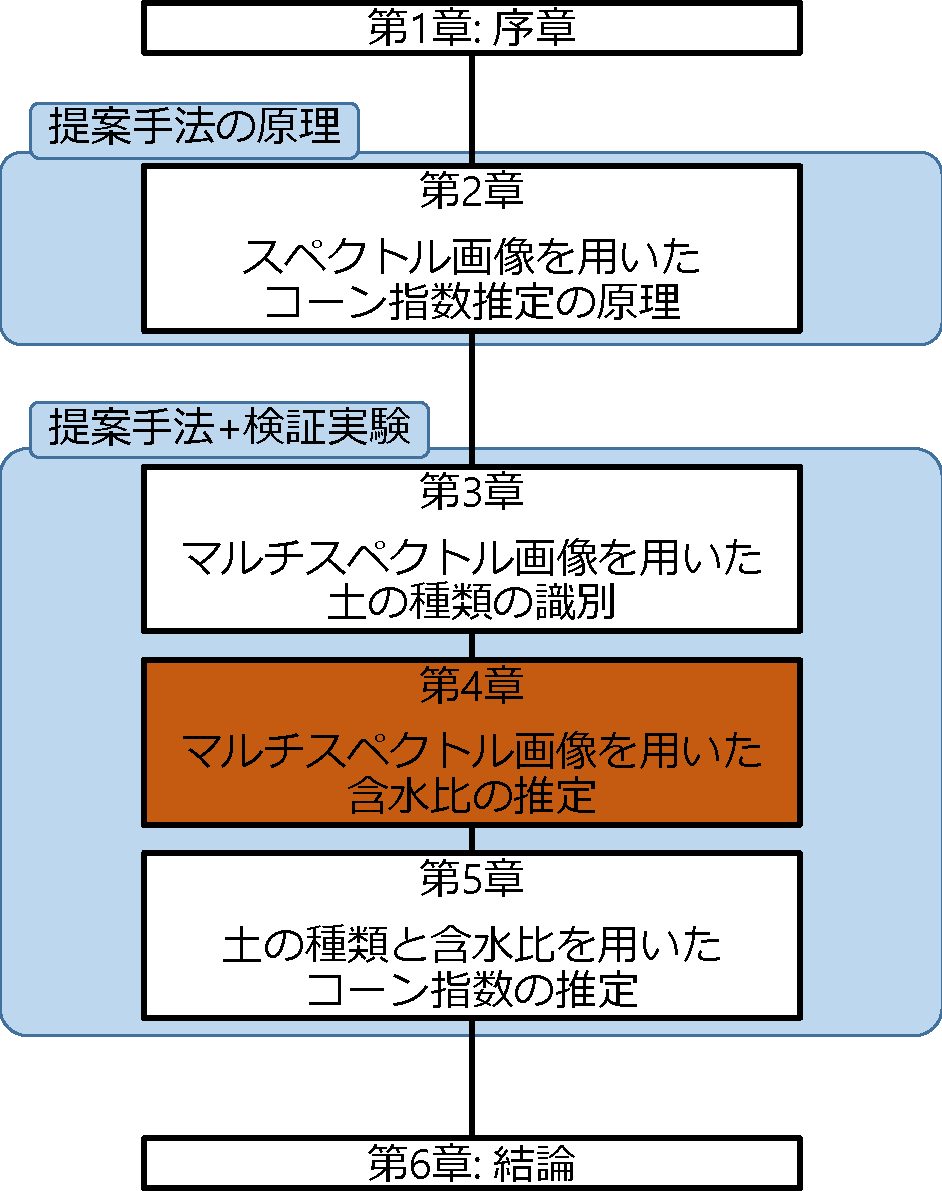
\includegraphics[width=8cm]{./Ch4_WaterContentEstimation/Fig/thesis_constitution_ch4_compressed.pdf}
	\caption{本章で解説する部分(茶色の部分)}\label{fig:thesis_constitution_ch4}
	\end{center}
\end{figure}

\clearpage

%==============================================================================
%分光反射率スペクトルを用いた含水比の推定
%==============================================================================
\section{分光反射率スペクトルを用いた含水比の推定}
\label{sec:EstimationFromSpectrum}

\subsection{含水比}
\label{ssec:WaterContent}

含水比は,土に含まれる水の量を示す土質パラメータであり,
土に含まれる土の粒子の質量に対する,同じ土に含まれる水の質量の比を示す土質パラメータである.
含水比を算出する式を\mbox{式(\ref{eq:watercontent_measurement})}に示す\cite{日本建設総合試験所2019}.

\begin{eqnarray}
含水比 = \frac{m_w}{m_s}, \label{eq:watercontent_measurement}
\end{eqnarray}

\mbox{式(\ref{eq:watercontent_measurement})}において,$m_w$,$m_s$は,それぞれ土に含まれる水の質量と土粒子の質量を示す.
$m_s$は,採取した土を乾燥炉に入れて水分を蒸発させることで測定する.
また,$m_w$は,採取した直後の土と乾燥させた後の土の質量の差から求められる.

土に含まれる空気,水,土粒子の関係を,図\ref{fig:watercontent_measurement}に示す.
土は,図\ref{fig:watercontent_measurement}に示すように,固体である土粒子,そして土粒子の間
に入り込んだ水と空気から出来ている.
\ref{ssec:ConeindexEstimation}項で述べた通り,土の粒子と水の質量の比である含水比が,コーン指数に大きく影響する.

\begin{figure}[bp]
      \begin{center}
            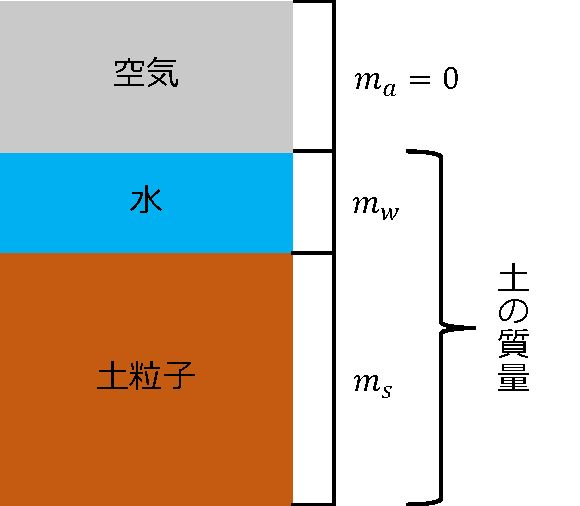
\includegraphics[width=7cm]{./Ch4_WaterContentEstimation/Fig/watercontent_measurement_compressed.pdf}
            \vspace{1cm}
            \caption{土に含まれる空気,水,土粒子の関係(\cite{日本建設総合試験所2019}を参考に作成)}
            \label{fig:watercontent_measurement}
      \end{center}
\end{figure}

\clearpage

\subsection{含水比と分光反射率スペクトルの関係}
\label{ssec:RelationshipBetweenSpectrumAndWaterContent}

% \ref{ssec:ConeindexEstimation}節で述べた通り,コーン指数は土の種類と含水比に大きな影響を受ける.
% そこで,コーン指数を非接触で推定するためには,土の種類の識別と含水比を非接触で推定する.

\ref{ssec:Spectrum}項で述べた通り,分光反射率スペクトルを用いた物質の種類の識別や状態の推定が可能である.
従って,含水比が変化した場合も,その土の分光反射率スペクトルが変動する.
水分子は,それを構成する酸素原子と水素原子の間の振動収縮と変角運動によって
特に近赤外の光を吸収することが知られている\cite{李2000}\cite{Lobell2002}\cite{Tian2015}.% 引用

含水比の違いによって,土の分光反射率スペクトルが異なるグラフを図\ref{fig:watercontent_and_spectrum_relationship}に示す.
この図において,縦軸が分光反射率,横軸が波長を示しており,描かれている3本の黒い曲線が土の分光反射率スペクトルを
示している.
この3本は同じ土の種類の分光反射率スペクトルであるが,上にある曲線から下にある曲線に行くに従って
含水比が高くなっており,上の曲線から順に,含水比が低い,真ん中,高い順に並んでいる.
そして,水が光を吸収しない波長帯が茶色で示され,水が光を吸収する波長帯である近赤外の波長帯が水色で示されている.
含水比が増えると土粒子の隙間に水が入り込み,空気と土の間の屈折率の差が減少するため,
空気中から土への入射光の内,反射せずに土の中に屈折して進入していく光の割合が増える.
従って,含水比の増加に伴って分光反射率スペクトルは全体的に低くなる.
しかし,その作用とは別に,水は水分子の酸素原子と水素原子の間の振動収縮と変角運動のために
近赤外の光を吸収するため,分光反射率スペクトル全体のなかでも,特に近赤外の % "波長"という単語はグラフの軸の説明にのみ使用
分光反射率が大きく減少する.
この性質を利用することで分光反射率スペクトルから含水比を推定する.
具体的には,図\ref{fig:watercontent_and_spectrum_relationship}のグラフにおいて,含水比が1番低い状態における2つの波長帯の分光反射率の差を$d_1$,
含水比が真ん中の状態における差を$d_2$,
含水比が1番高い状態における差を$d_3$とすると,
\begin{eqnarray}
d_1 > d_2 > d_3, \label{eq:spectrumDiff}
\end{eqnarray}
となっていることが分かる.
この\mbox{式(\ref{eq:spectrumDiff})}より,含水比が増加すると,
水が光を吸収する近赤外の波長帯の分光反射率から水が光を吸収しない波長帯の分光反射率を
引いた差は逆に減少することが分かる.
これを利用して含水比を推定する.

\begin{figure}[b]
      \begin{center}
            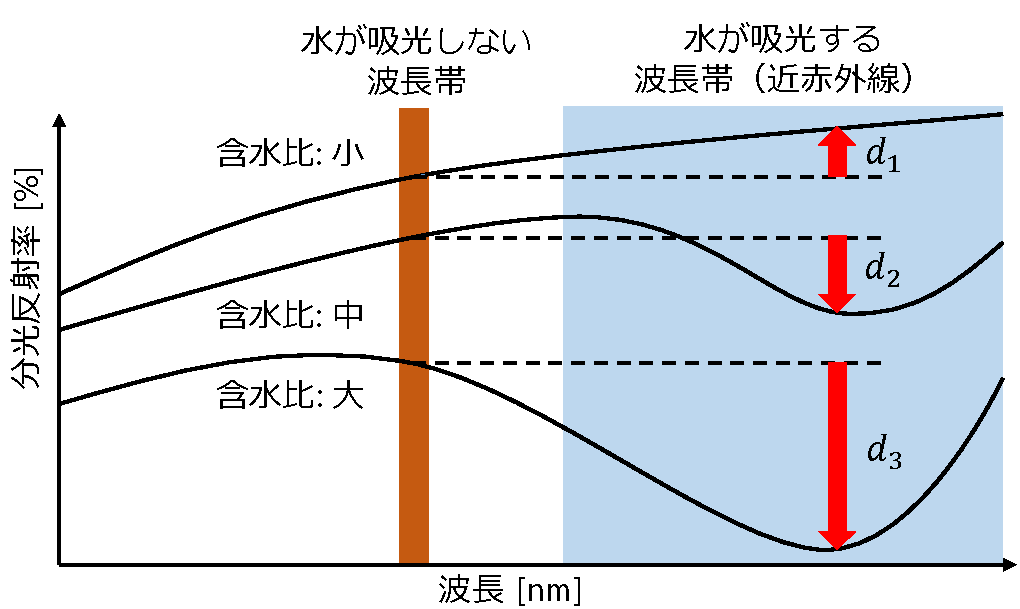
\includegraphics[width=12cm]{./Ch4_WaterContentEstimation/Fig/watercontent_and_spectrum_relationship_compressed.pdf}
            \caption{同一種類の土における含水比の増加に伴う分光反射率の減少}
            \label{fig:watercontent_and_spectrum_relationship}
            \vspace{3cm}
      \end{center}
\end{figure}



水分子が近赤外の光を吸収する原因となる酸素原子と水素原子の間の振動収縮と変角運動は,
水分子の周囲に存在する他の水分子との水素結合の数と方向に大きく左右される\cite{中島2015}.
そしてその水素結合の数と方向は温度や湿度に大きく影響される\cite{角田2013}.
従って,水は,温度や湿度によって最も光を吸収する波長帯を変化させるため,
近赤外において広い範囲の光を吸収する.

% ここにもう1つ項(土の種類の識別に必要な分光反射率スペクトルの要件)を入れて,波長分解能についてより詳しく述べる
% なぜマルチスペクトル画像を使用する必要があるのか?

従って,近赤外の光の分光反射率を用いて含水比を推定するためには,
近赤外の幅広い範囲の光を取得するスペクトル画像を用いる必要がある.
そのため,本研究では,スペクトル画像のなかでも,入射光を分光させる波長帯の数が少なく,
近赤外の幅広い範囲の光を取得することが
できるマルチスペクトル画像を用いる.

\clearpage

%==============================================================================
%マルチスペクトル画像の解析
%==============================================================================
\section{マルチスペクトル画像の解析}
\label{sec:AnalysisOfMultispectralImage}

\subsection{波長帯の数が少ないマルチスペクトル画像}
\label{ssec:MultispectralImage}

マルチスペクトル画像とは,\ref{sec:HyperAndMultiImages}で述べた通り,一般的なRGB画像が取得するR,G,Bの3波長帯以外の波長帯も取得するスペクトル画像である.
% 一般的には,分光させた波長帯の数は4以上9以下であると言われている.% マルチスペクトル画像の波長数が4~9であることはここで終わり
取得する波長帯の数が少ないマルチスペクトル画像は,スペクトル画像が使われ出した当初から使用されており,
顔の色素の分布や建材の塗装量の調査,工業製品の外観検査に使用されている\cite{中野1996}\cite{長田2004}\cite{田代2013}.% 引用

マルチスペクトル画像の中でも,
取得する波長帯の数が少ないマルチスペクトル画像は,一般的に異なる光学フィルタを装着した,
% 複数のカメラ
並列に並んだ複数の撮像素子
を用いて各波長帯の光の強さを記録する.
従って,同じ位置にある画素であっても,波長帯が異なると映している場所が異なる.
そこで,\ref{ch:SoilTypeDiscrimination}章で使用した,取得する波長帯の数が非常に多いスペクトル画像の場合とは違って,画素ごとに分光反射率スペクトルを取得するのではなく,
まず水が光を吸収する近赤外の波長帯とそれ以外の水が光を吸収しない波長帯の,2つの波長帯を取得した
後,それぞれの波長帯で同じ場所を映している画素を選んで分光反射率を計算する.
最後に,その差を用いて含水比を推定する.
% \begin{figure}[p]
% 	\begin{center}
% 	\centering
% 	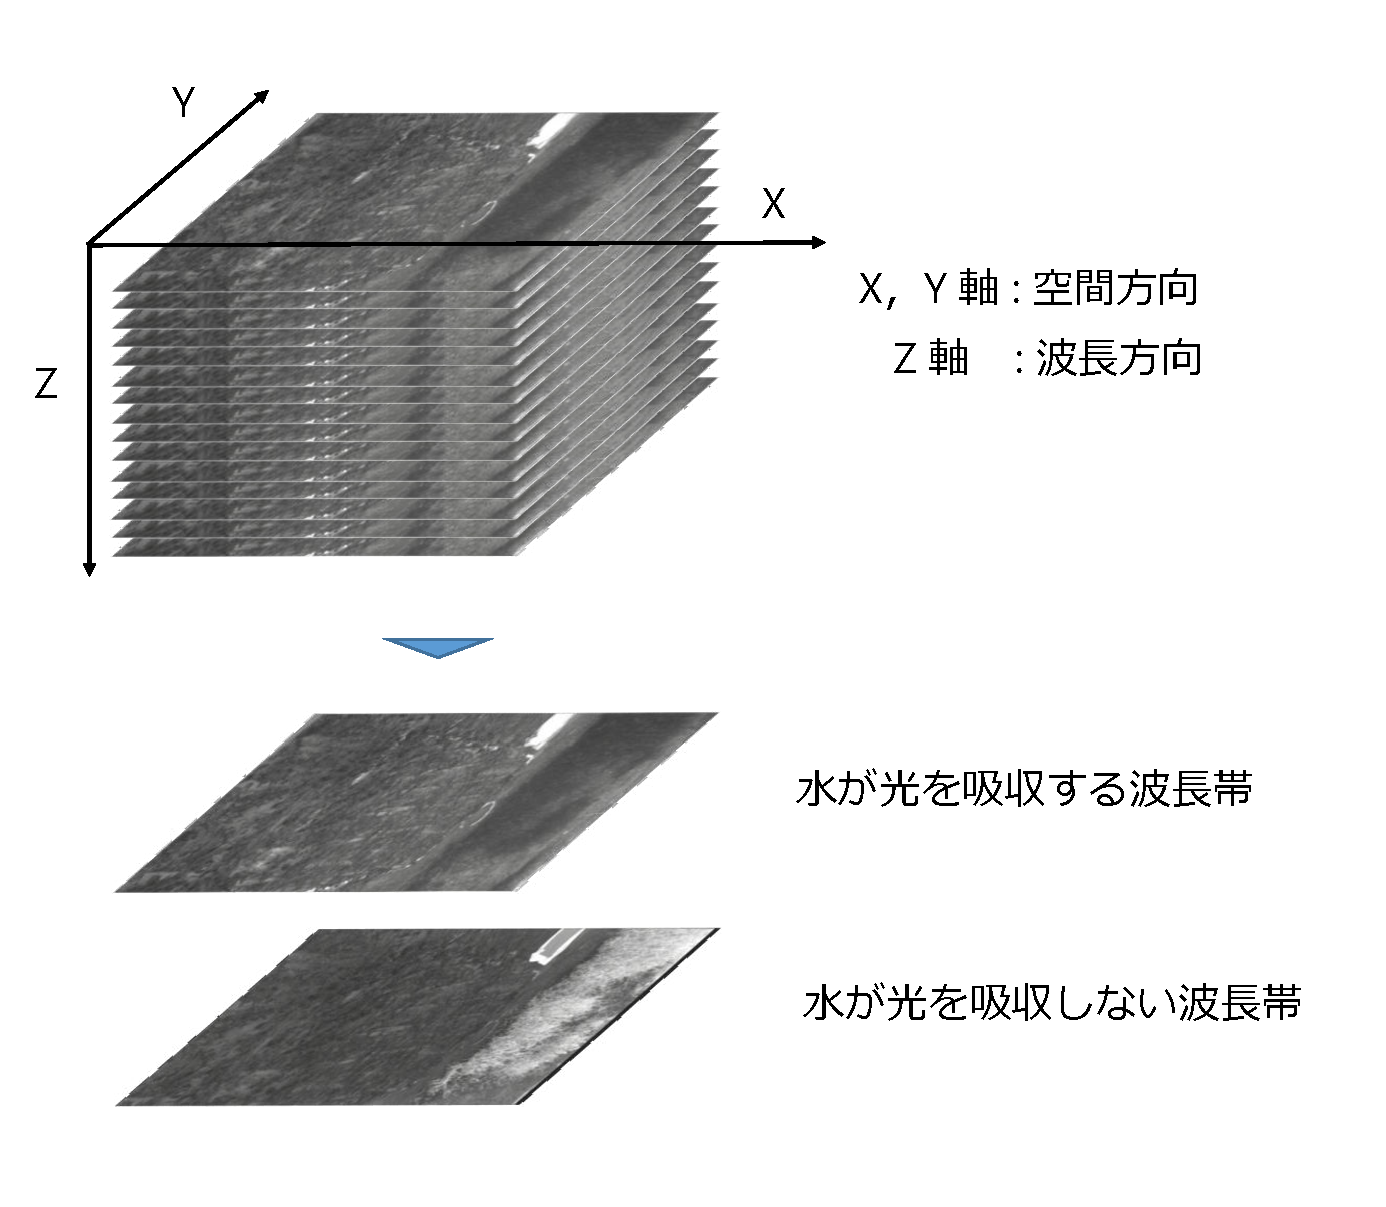
\includegraphics[width=12cm]{./Ch4_WaterContentEstimation/Fig/spectral_image_extraction_compressed.pdf}
% 	\caption{マルチスペクトル画像からの2つの波長帯の抽出}\label{fig:spectral_image_extraction}
% 	\end{center}
% \end{figure}

\clearpage

\subsection{分光反射率の解析}
\label{ssec:AnalysisOfSpectrum}

本研究では,水が光を吸収する近赤外の波長帯として900 $\sim$ 1700nmの波長帯を,水が光を吸収しない波長帯として570nmの波長帯を使用する.
同じ種類の土で含水比が異なるサンプルを作り,屋外において,
それぞれのサンプルを太陽光を光源として撮影したマルチスペクトル画像から取得した900 $\sim$ 1700nmの波長帯と570nmの波長帯
の分光反射率をプロットしたグラフを,図\ref{fig:watercontent_and_spectrum_graph}に示す.
図\ref{fig:watercontent_and_spectrum_graph}のグラフにおいて,縦軸が含水比,横軸が分光反射率を示す.
また,図\ref{fig:watercontent_and_spectrum_graph}のグラフに示されている赤いひし形が,同一種類の土で含水比の異なるサンプルを撮影した各マルチスペクトル画像の570nmの波長帯で計算した分光反射率を
プロットしており,黒いひし形が,同一種類の土で含水比の異なるサンプルを撮影した各マルチスペクトル画像の900 $\sim$ 1700nmの波長帯で計算した分光反射率を示す.
さらに,上記で解説した2つの波長帯の分光反射率の間にある赤い矢印が,2つの波長帯の分光反射率の差$d$を示す.

次に,その2つの波長帯の分光反射率の差と含水比を比較したグラフを,図\ref{fig:watercontent_and_spectrumDiff_graph}に示す.
図\ref{fig:watercontent_and_spectrumDiff_graph}のグラフにおいて,縦軸は先ほどと同じ含水比を示すが,横軸は2つの波長帯の分光反射率の差$d$を示す.
なお,横軸は2つの波長帯の分光反射率の単なる差を示すので,単位は図\ref{fig:watercontent_and_spectrum_graph}のグラフの横軸と同じく$\%$となる.
また,図\ref{fig:watercontent_and_spectrumDiff_graph}のグラフに示されている黒い点は,
各含水比に対する,図\ref{fig:watercontent_and_spectrum_graph}のグラフで示された570nmの波長帯の分光反射率と900 $\sim$ 1700nmの波長帯の分光反射率の差を示す.
この図\ref{fig:watercontent_and_spectrumDiff_graph}のグラフより,含水比が減少するに伴って,2つの波長帯の分光反射率の差$d$が増加していることが分かる.
そこで,このグラフに近似線をフィッティングし,そのフィッティングされた近似線を用いることによって,
マルチスペクトル画像から
含水比を推定する.

\begin{figure}[p]
	\begin{center}
		\begin{tabular}{c}

			\begin{minipage}[t]{\linewidth}
			\hspace{1.5cm}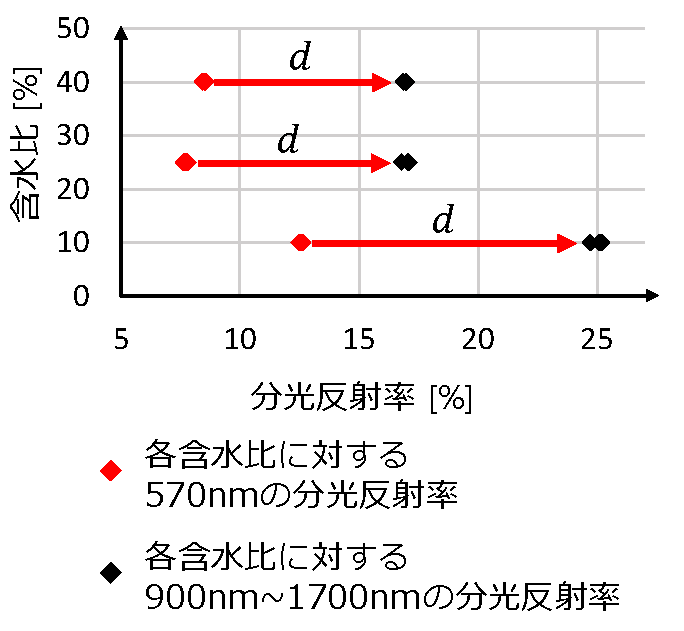
\includegraphics[width=8cm]{./Ch4_WaterContentEstimation/Fig/watercontent_and_spectrum_graph_compressed.pdf}
			\caption{含水比と2つの波長帯の分光反射率の関係}\label{fig:watercontent_and_spectrum_graph}
			\vspace{2cm}
			\end{minipage}

			\\

			\begin{minipage}[b]{\linewidth}
			\hspace{1.5cm}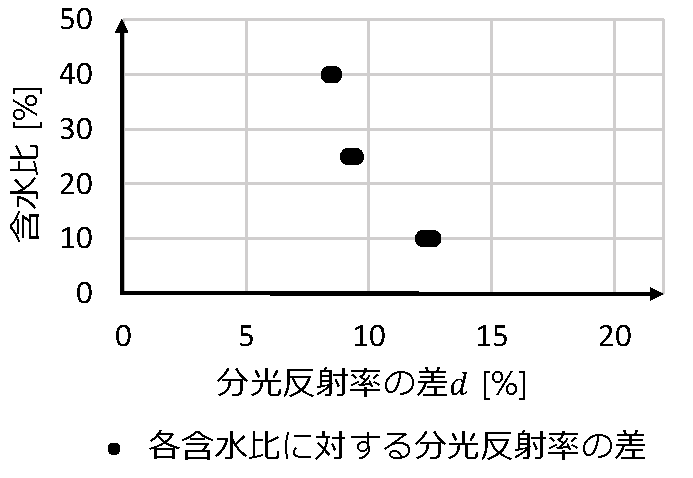
\includegraphics[width=8cm]{./Ch4_WaterContentEstimation/Fig/watercontent_and_spectrumDiff_graph_compressed.pdf}
			\caption{含水比と分光反射率の差の関係}\label{fig:watercontent_and_spectrumDiff_graph}
			\end{minipage}

		\end{tabular}
	\end{center}
\end{figure}

\clearpage

\subsection{モデルフィッティング}
\label{ssec:ModelFitting}

\ref{ssec:AnalysisOfSpectrum}項で示した,2つの波長帯の分光反射率の差$d$と含水比の関係を示す図\ref{fig:watercontent_and_spectrumDiff_graph}のグラフにフィッティングされる近似線として,本研究では指数近似線を使用する.
水の増加に伴い,水の中を吸収されずに透過する光の割合は,急激に減少する.
従って,土の表面を濡れた部分が覆う程に含水比が増加するまでは近赤外の光の分光反射率は急激に減少し,
その後の減少は緩やかになるため,
図\ref{fig:watercontent_and_spectrumDiff_graph}に示すように,含水比が低い内は,含水比の増加に伴って2つの波長帯の分光反射率の差$d$は最初は急激に負の方向へ変化し,含水比が高くなると,含水比の増加に伴う$d$の負の方向への変化の度合いは緩やかになる.
そこで,2つの波長帯の分光反射率の差$d$を独立変数とし含水比を従属変数とする近似線に指数近似線を使用する.
先ほどの図\ref{fig:watercontent_and_spectrumDiff_graph}のグラフに指数近似線をフィッティングさせた様子を図\ref{fig:model_fitting}に示す.
図\ref{fig:model_fitting}のグラフにおいて,縦軸と横軸は,\ref{ssec:AnalysisOfSpectrum}項の図\ref{fig:watercontent_and_spectrumDiff_graph}と同様にそれぞれ含水比と570nmの波長帯の分光反射率と900 $\sim$ 1700nmの波長帯の分光反射率の差を示しており,グラフ中の黒い点も図\ref{fig:watercontent_and_spectrumDiff_graph}と同様に,各含水比に対する570nmの波長帯の分光反射率と900 $\sim$ 1700nmの波長帯の分光反射率の差を示す.
また,赤い曲線は黒い点に近似させた指数近似線を示す.
% 図\ref{fig:model_fitting}のグラフに示された決定係数$R^2 = 0.9792$より,指数近似線$y = 583.2\mathrm{e}^{-0.327x}$がフィッティングされていることが分かる.
% それは,この指数近似線の決定係数の$R^2 = 0.9792$を見ても分かる.
本研究では,予めそれぞれの土の種類に対して,含水比が異なるサンプルを作成してマルチスペクトル画像を撮影することによって,
含水比と570nmの波長帯の分光反射率と900 $\sim$ 1700nmの波長帯の分光反射率の差の関係を取得する.
そしてその関係を示すグラフにおいて指数近似線によるフィッティングを行い,
その指数近似線を用いて新たに撮影したマルチスペクトル画像から含水比を推定する.

\begin{figure}[p]
	\begin{center}
	\centering
	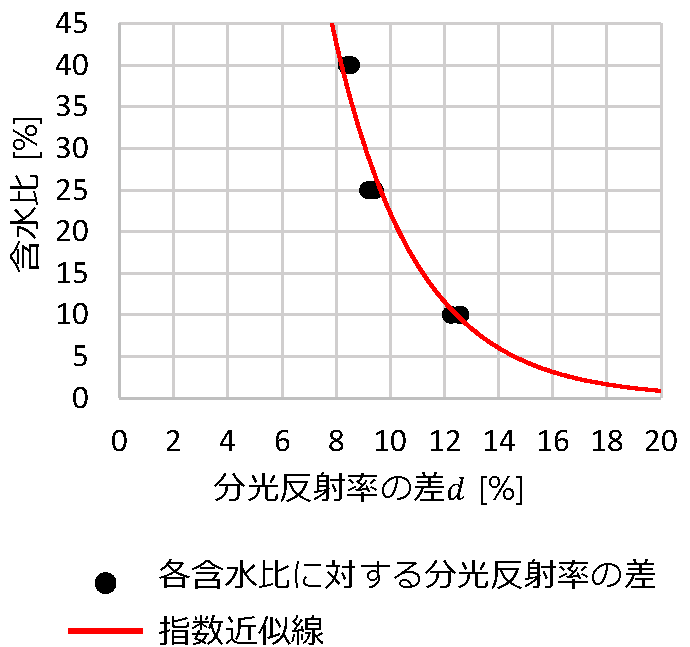
\includegraphics[width=8cm]{./Ch4_WaterContentEstimation/Fig/model_fitting_compressed.pdf}
	\caption{含水比と分光反射率の差の関係への指数近似線のフィッティング}\label{fig:model_fitting}
	\vspace{0.5cm}
	\end{center}
\end{figure}

\clearpage


%==============================================================================
%含水比を推定する検証実験
%==============================================================================
\section{含水比を推定する検証実験}
\label{sec:PreliminaryExperimentOfEstimation}

\ref{sec:EstimationFromSpectrum}節と\ref{sec:AnalysisOfMultispectralImage}節で解説した,
マルチスペクトル画像から取得した水が光を吸収する近赤外の波長帯と水が光を吸収しない波長帯の2つの波長帯の分光反射率の差を用いた,
含水比推定の手法の有効性を確認するため,
検証実験を行った.

\subsection{実験環境}
\label{ssec:EstimationExperimentSetting}

今回の検証実験の目的は,水による光の吸収度合いが異なる2つの波長帯の分光反射率の差を用いて,含水比を推定できるか確認することである.
そこで,同じ種類の土に対して含水比が10\%,25\%,40\%の合計3つのサンプルを用意し,
そして,屋外でそのサンプルのマルチスペクトル画像を撮影した.
マルチスペクトル画像を撮影した様子を図\ref{fig:watercontent_estimation_experiment_setting}に示す.
図\ref{fig:watercontent_estimation_experiment_setting}に示す通り,同じ種類だが異なる含水比の土のサンプル3つと,分光反射率スペクトルが分かっている校正用シートを
並べて撮影した.
サンプルと校正用シートの並び順を図\ref{fig:watercontent_estimation_experiment_sample_arrangement}に示す.
% そして,マルチスペクトル画像を撮影するためのマルチスペクトルカメラを土を入れた容器の直情に配置して,撮影を行った.
また,今回の検証実験で使用したマルチスペクトルカメラは,TETRACAM製のMacawである.
Macawの写真を図\ref{fig:multispectral_camera}に示す.
また,Macawの具体的な仕様を表\ref{tbl:multispectral_camera}に示す.

\begin{figure}[p]
	\begin{center}
		\begin{tabular}{c}

			\begin{minipage}[t]{\linewidth}
			\hspace{3cm}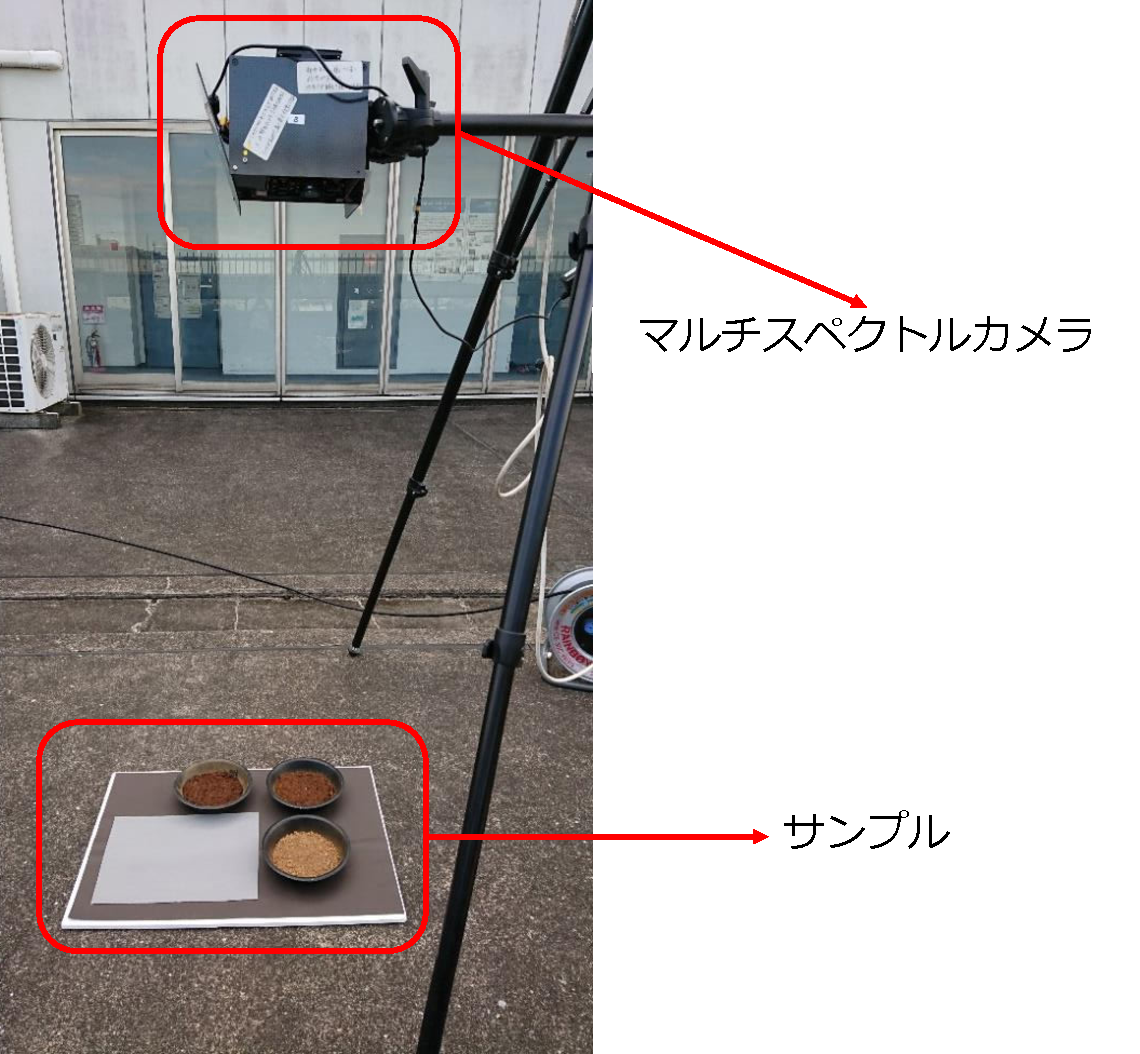
\includegraphics[width=9cm]{./Ch4_WaterContentEstimation/Fig/watercontent_estimation_experiment_setting_compressed.pdf}
			\caption{含水比推定の検証実験における撮影機材の配置}\label{fig:watercontent_estimation_experiment_setting}
			\vspace{2cm}
			\end{minipage}

			\\

			\begin{minipage}[b]{\linewidth}
			\centering
			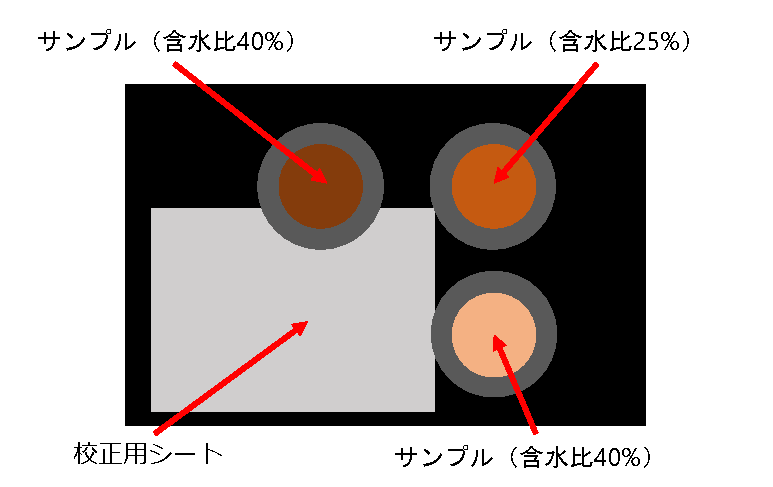
\includegraphics[width=12cm]{./Ch4_WaterContentEstimation/Fig/watercontent_estimation_experiment_sample_arrangement_compressed.pdf}
			\caption{含水比推定の検証実験における異なる含水比のサンプルの配置}\label{fig:watercontent_estimation_experiment_sample_arrangement}
			\end{minipage}

		\end{tabular}
	\end{center}
\end{figure}


\begin{figure}[p]
	\begin{center}
		\begin{tabular}{c}

			\begin{minipage}[t]{\linewidth}
			\hspace{4cm}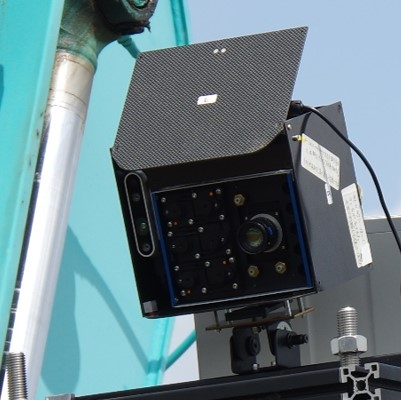
\includegraphics[width=6cm]{./Ch4_WaterContentEstimation/Fig/multispectral_camera.jpg}
			\caption{Macaw}\label{fig:multispectral_camera}
			\vspace{2cm}
			\end{minipage}

			\\

			\begin{minipage}[b]{\linewidth}

			\tblcaption{Macawの仕様}\label{tbl:multispectral_camera}

				\hspace{4cm} \begin{tabular}{|c|c|} \hline % 表の位置が左に寄りすぎないように調整
				製品名 & Macaw \\
				(メーカー) & (TETRACAM) \\ \hline
				波長 & 490nm, 570nm, 671nm \\ 
				     & 800nm, 900nm, 950nm \\
				     & 900 $\sim$ 1700nm \\ \hline
				波長帯数 & 7 \\ \hline
				\end{tabular}
			\end{minipage}

		\end{tabular}
	\end{center}
\end{figure}
 
\clearpage

\subsection{実験データ}
\label{ssec:EstimationExperimentalProcedure}

今回の実証実験では,\ref{sec:PreliminaryExperimentOfDiscrimination}節で解説した土の種類を識別する検証実験で使用した10種類の土のうち,
粘性土と火山灰質粘性土によって構成される5種類の細粒土を使用した.% この5種類の細粒度は,粘性土と呼ばれる土に属している.
砂質土や礫質土が,含水比の増減に関係なく建設機械の走破が可能な程度のコーン指数を維持するのに対し,
火山灰質粘性土も含む粘性土は,含水比が上昇すると建設機械の走破が困難になるほどコーン指数を低下させる土であることが知られている\cite{Meyer1961}.% "コーン指数"には低下という言葉を使用する
そこで,この検証実験においても,5種類の粘性土を対象として含水比推定の検証実験を行った.
今回使用する粘性土は,\ref{sec:PreliminaryExperimentOfDiscrimination}節で使用した10種類の土のうちの,
A, B, D, F, Gの粘性土である.
この5種類の粘性土のRGB画像を図\ref{fig:watercontent_estimation_experiment_data}に示す.

% \begin{figure}[p]
% 	\begin{center}
% 	\centering
% 	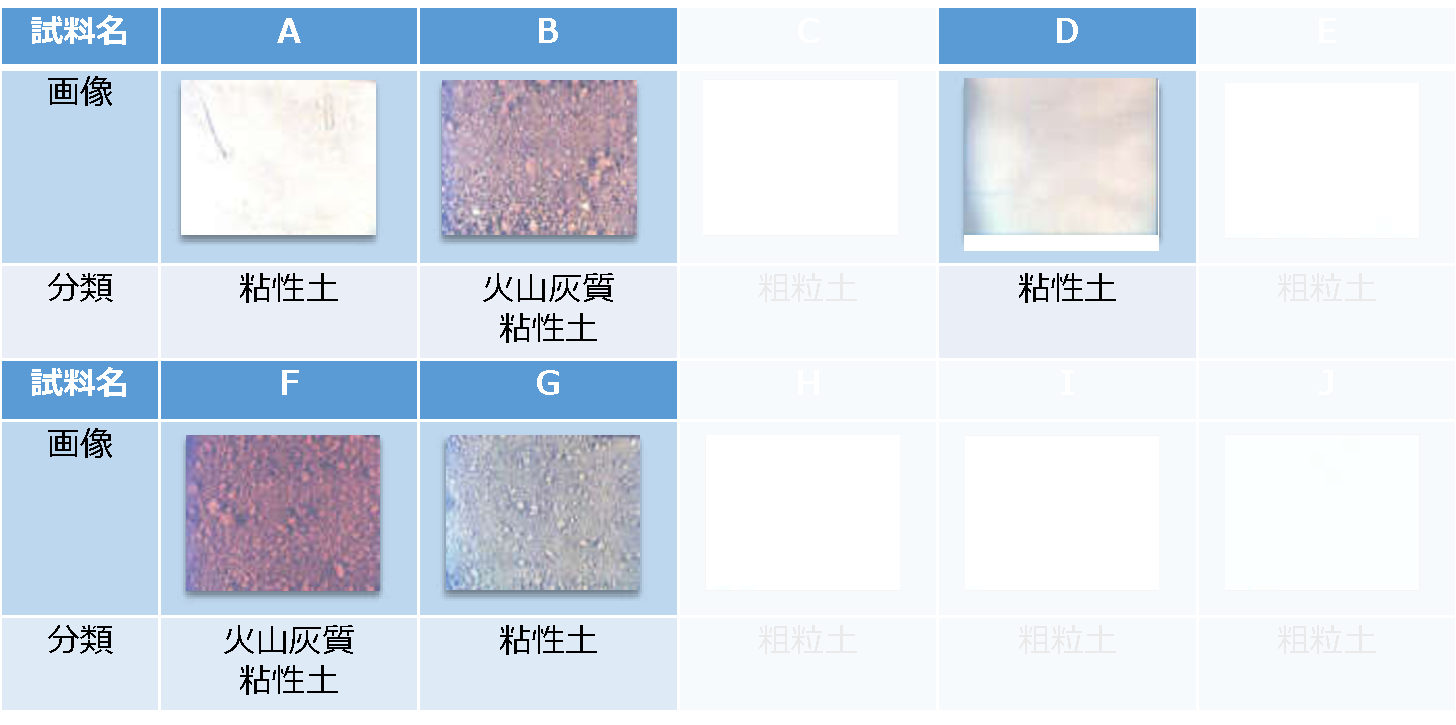
\includegraphics[width=15cm]{./Ch4_WaterContentEstimation/Fig/watercontent_estimation_experiment_data_compressed.pdf}
% 	\caption{含水比推定の検証実験用のデータ}\label{fig:watercontent_estimation_experiment_data}
% 	\end{center}
% \end{figure}

\begin{figure}[b]
	\begin{center}
		\begin{tabular}{c}

			\begin{minipage}[t]{0.33\linewidth}
			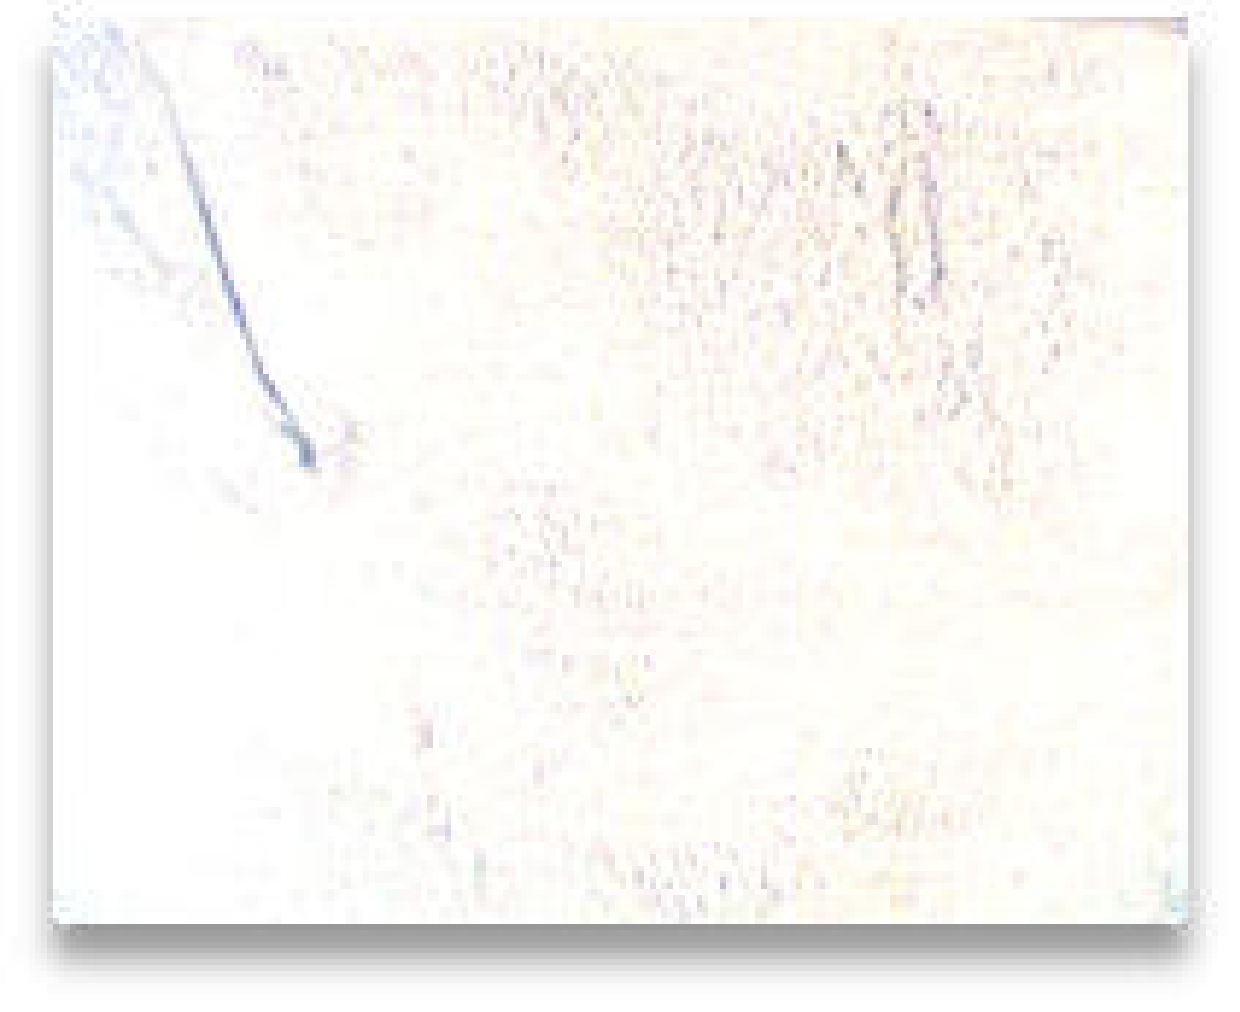
\includegraphics[width=4cm]{./Ch3_SoilTypeDiscrimination/Fig/A_Fu_image_compressed.pdf}
			\caption*{(a)土の種類A(粘性土)}%\label{fig:spectrum_for_different_soiltype}
			% \vspace{2cm}
			\end{minipage}

			\begin{minipage}[t]{0.33\linewidth}
			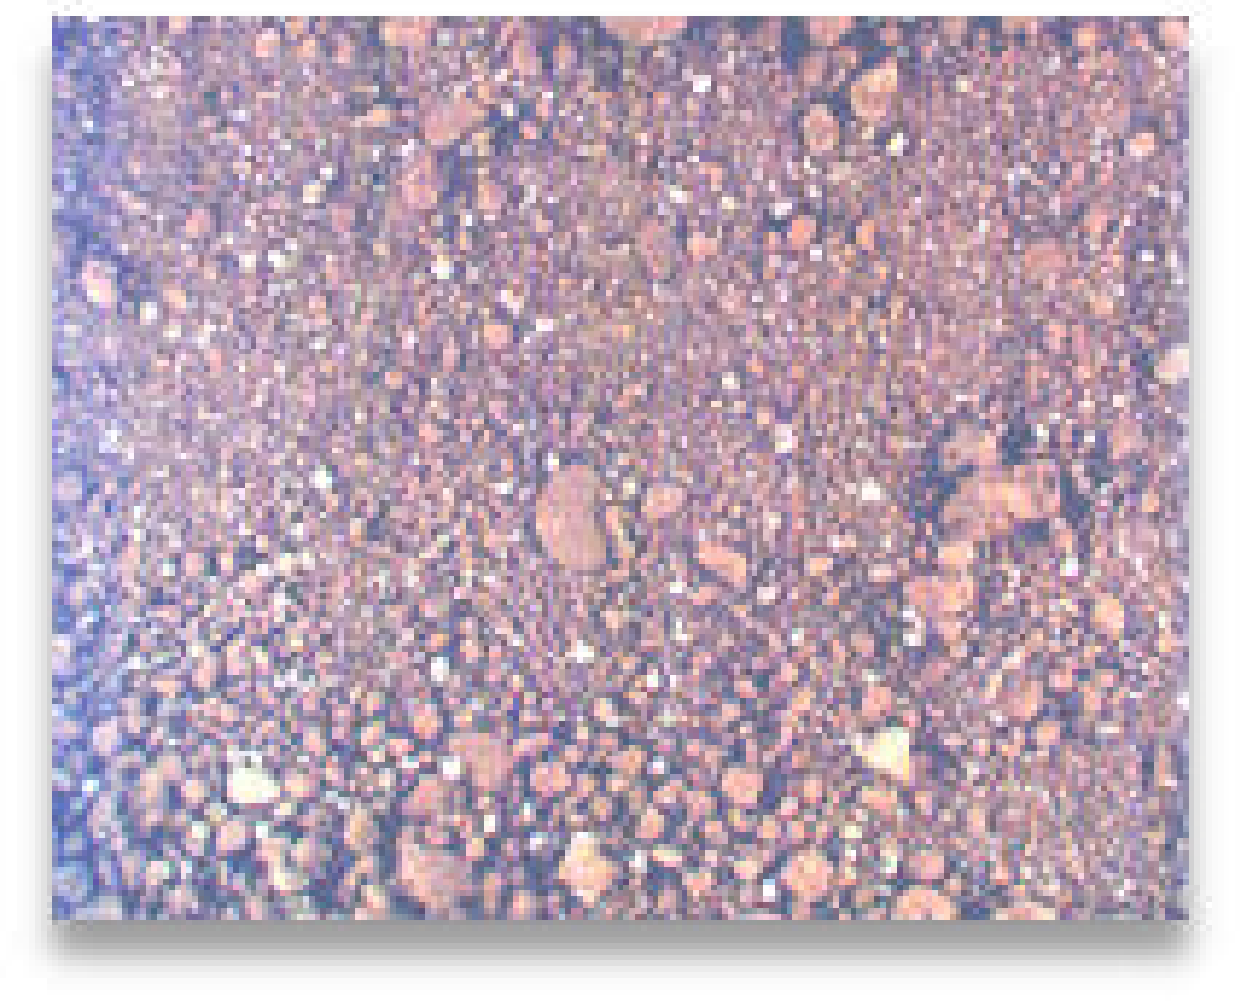
\includegraphics[width=4cm]{./Ch3_SoilTypeDiscrimination/Fig/B_Is_image_compressed.pdf}
			\caption*{(b)土の種類B(火山灰質粘性土)}
			\end{minipage}

			\hfill

			% \begin{minipage}[t]{0.33\linewidth}
			% 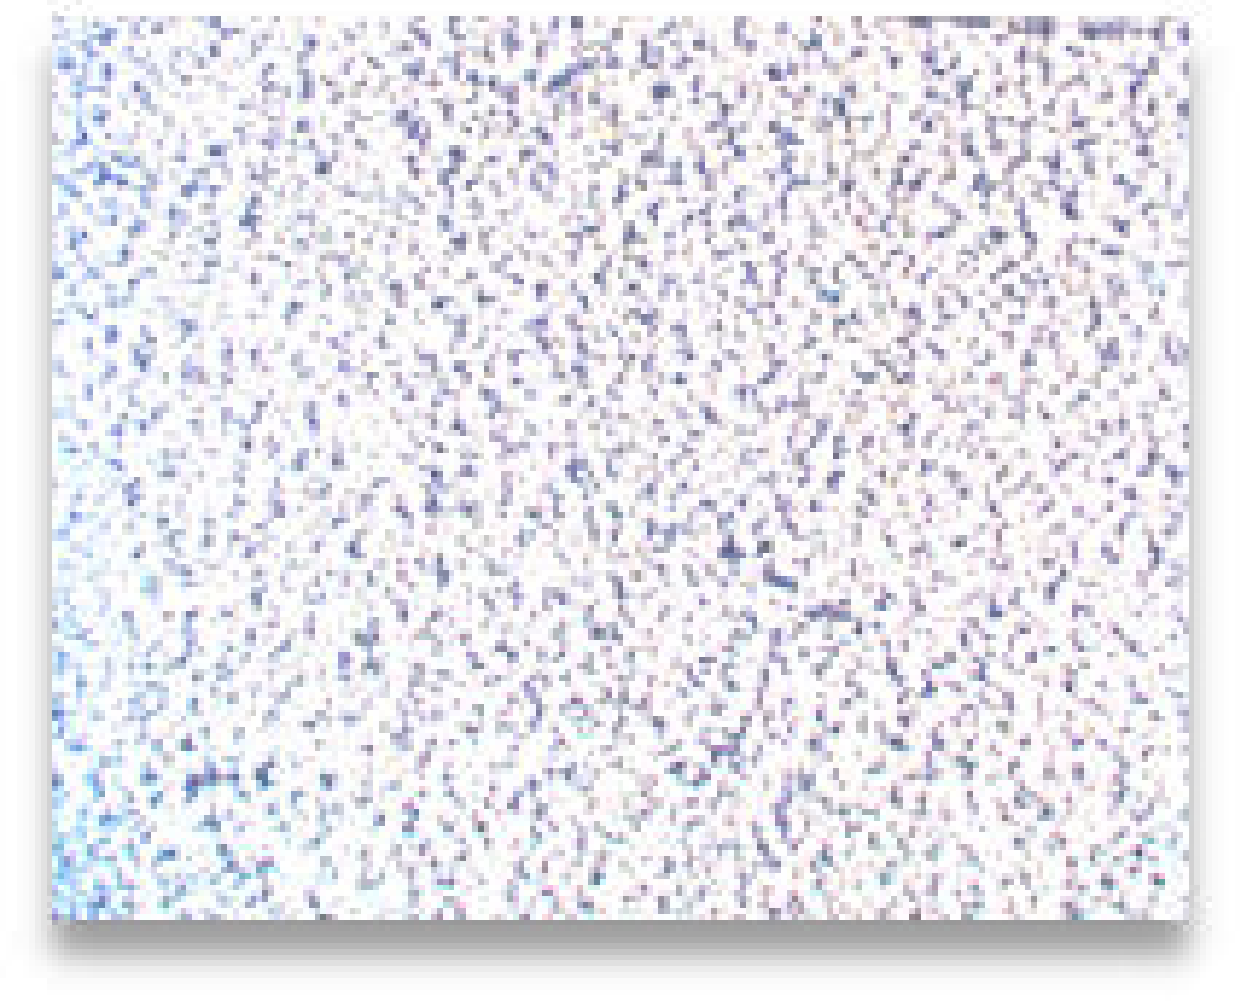
\includegraphics[width=4cm]{./Ch3_SoilTypeDiscrimination/Fig/C_K1_image_compressed.pdf}
			% \caption*{土の種類C(粗粒土の1種)}
			% \end{minipage}

			

			\begin{minipage}[t]{0.33\linewidth}
			\includegraphics[width=4cm]{./Ch3_SoilTypeDiscrimination/Fig/D_K9_image_compressed.pdf}
			\caption*{(c)土の種類D(粘性土)}%\label{fig:spectrum_for_different_soiltype}
			% \vspace{2cm}
			\end{minipage}

			\\

			% \begin{minipage}[t]{0.33\linewidth}
			% \includegraphics[width=4cm]{./Ch3_SoilTypeDiscrimination/Fig/E_Ko_image_compressed.pdf}
			% \caption*{土の種類E(粗粒土の1種)}
			% \end{minipage}

			% \hfill

			\begin{minipage}[t]{0.33\linewidth}
			\includegraphics[width=4cm]{./Ch3_SoilTypeDiscrimination/Fig/F_Lo_image_compressed.pdf}
			\caption*{(d)土の種類F(火山灰質粘性土)}
			\end{minipage}

			% \\

			\begin{minipage}[t]{0.33\linewidth}
			\includegraphics[width=4cm]{./Ch3_SoilTypeDiscrimination/Fig/G_Mi_image_compressed.pdf}
			\caption*{(e)土の種類G(粘性土)}%\label{fig:spectrum_for_different_soiltype}
			% \vspace{2cm}
			\end{minipage}

			% \begin{minipage}[t]{0.33\linewidth}
			% \includegraphics[width=4cm]{./Ch3_SoilTypeDiscrimination/Fig/H_Oh_image_compressed.pdf}
			% \caption*{土の種類H(粗粒土の1種)}
			% \end{minipage}

			% \hfill

			% \begin{minipage}[t]{0.33\linewidth}
			% \includegraphics[width=4cm]{./Ch3_SoilTypeDiscrimination/Fig/I_Sa_image_compressed.pdf}
			% \caption*{土の種類I(粗粒土の1種)}
			% \end{minipage}

			% \\

			% \begin{minipage}[t]{0.33\linewidth}
			% \includegraphics[width=4cm]{./Ch3_SoilTypeDiscrimination/Fig/J_Sc_image_compressed.pdf}
			% \caption*{土の種類J(粗粒土の1種)}
			% \end{minipage}

		\end{tabular}
		\caption{含水比推定の検証実験用のデータ}\label{fig:watercontent_estimation_experiment_data}
	\end{center}
\end{figure}

\clearpage


\subsection{実験結果}
\label{ssec:EstimationResult}

\ref{sec:AnalysisOfMultispectralImage}節で解説した手法を用いて,
900 $\sim$ 1700nmの波長帯と570nmの波長帯の分光反射率の差に指数近似線をフィッティングさせた様子を
図\ref{fig:watercontent_estimation_fitting}に示す.
図\ref{fig:watercontent_estimation_fitting}にある各グラフは,\ref{ssec:AnalysisOfSpectrum}節で示した図\ref{fig:model_fitting}のグラフと同様に,
縦軸は含水比を示しており,横軸は2つの波長帯の分光反射率の差を示している.
また,各グラフにおいて,黒い点が撮影したマルチスペクトル画像から取得した900 $\sim$ 1700nmの波長帯と570nmの波長帯の分光反射率の差と
含水比の関係をプロットした点であり,赤い曲線がそのプロットされた黒い点にフィッティングされた指数近似線を示す.
図\ref{fig:watercontent_estimation_fitting}にある各グラフおよびそのグラフに示された決定係数$R^2$から分かる通り,今回の含水比推定の検証実験で使用した5種類の粘性土において,モデルフィッティングが成功したことが分かる.
% 各グラフに示された決定係数$R^2$からもそれが分かる.

\begin{figure}[p]
	\begin{center}
		\begin{tabular}{c} % 隣り合う図がずれないようにする

			\hspace{-1cm}\begin{minipage}[b]{0.5\linewidth}
			\centering
			\includegraphics[width=7cm]{./Ch4_WaterContentEstimation/Fig/image_Fu(A)watercontent_spectrum_relationship_compressed.pdf}
			\caption*{(a)土の種類A}
			\end{minipage}

			\hfill

			\begin{minipage}[b]{0.5\linewidth}
			\centering
			\includegraphics[width=7cm]{./Ch4_WaterContentEstimation/Fig/image_Is(B)watercontent_spectrum_relationship_compressed.pdf}
			\caption*{(b)土の種類B}
			\end{minipage}

			\\

			\hspace{-1cm}\begin{minipage}[b]{0.5\linewidth}
			\centering
			\includegraphics[width=7cm]{./Ch4_WaterContentEstimation/Fig/image_K9(D)watercontent_spectrum_relationship_compressed.pdf}
			\caption*{(c)土の種類D}
			\end{minipage}

			\hfill

			\begin{minipage}[b]{0.5\linewidth}
			\centering
			\includegraphics[width=7cm]{./Ch4_WaterContentEstimation/Fig/image_Lo(F)watercontent_spectrum_relationship_compressed.pdf}
			\caption*{(d)土の種類F}
			\end{minipage}

			\\

			\hspace{-1cm}\begin{minipage}[b]{0.5\linewidth}
			\centering
			\includegraphics[width=7cm]{./Ch4_WaterContentEstimation/Fig/image_Mi(G)watercontent_spectrum_relationship_compressed.pdf}
			\caption*{(e)土の種類G}
			\end{minipage}

			\hfill

			\begin{minipage}[b]{0.5\linewidth}
			\centering
			\vspace{-3cm}
			\includegraphics[width=5cm]{./Ch4_WaterContentEstimation/Fig/legend_of_watercontent_spectrum_relationship_compressed.pdf}
			\end{minipage}

		\end{tabular}
	\caption{含水比推定のための指数近似線によるフィッティング}\label{fig:watercontent_estimation_fitting}
	\end{center}
\end{figure}

\clearpage


\subsection{考察}
\label{ssec:EstimationConsideration}

\ref{ssec:EstimationResult}項で示した含水比推定の検証実験の結果より,
マルチスペクトル画像から取得した,水が光を吸収する近赤外の波長帯と,水が光を吸収しない波長帯の分光反射率の,2つの分光反射率の差を用いた
含水比の推定が可能であることが分かった.
水が近赤外の光を吸収することを利用した含水比の推定手法が上手くいった原因は,
マルチスペクトル画像を用いて近赤外の広い範囲の光を1つの波長帯として分光させたため,
温度や湿度の変動による近赤外の光を吸収する波長帯の多少の変動には頑強であったためである.

しかし,図\ref{fig:watercontent_estimation_fitting}(d)のFの土のグラフに示した,含水比が40$\%$や25$\%$のプロットのように,
水が光を吸収する近赤外の波長帯と水が光を吸収しない波長帯の分光反射率の差と含水比の関係をプロットした点の一部は,
近似線から離れたところにあることも分かった.
これは,\ref{ssec:RelationshipBetweenSpectrumAndWaterContent}項で述べたように,
含水比の増加に伴い,
空気と土の間の屈折率の差が減少するため,
空気中から土への入射光の内,反射せずに土の中に屈折して進入していく光の割合が増えるため,
水が光を吸収しない波長帯の分光反射率も含水比の増加に伴い変動するためである.
水が光を吸収しない波長帯の分光反射率が大きく変動すると,
水が光を吸収する近赤外の波長帯と光を吸収しない波長帯の差に影響を与え,
分光反射率の差を用いた含水比の推定の難易度が上昇する.
この変動を抑制するためには,
近赤外線以外の,水が光を吸収しない波長帯に,
本論文の中で使用した570nmの波長帯よりも,含水比の増加に伴う分光反射率の変動の少ない波長帯を探索する必要がある.

\newpage

%==============================================================================
%おわりに
%==============================================================================
\section{おわりに}

本章では,本研究で提案した非接触での走破性判定のための手法の2つ目のステップである,
スペクトル画像を用いた含水比の推定の詳細について述べた.

まず,\ref{sec:EstimationFromSpectrum}節において,
水分子がその構成原子である酸素原子と水素原子の間の振動収縮と変角運動によって
近赤外の光を吸収することを利用し,水が光を吸収する近赤外の波長帯と水が光を吸収しない波長帯の分光反射率の差を用いて
含水比を推定することを述べた.

次に,\ref{sec:AnalysisOfMultispectralImage}節において,
マルチスペクトル画像から取得した分光反射率の差を用いて含水比を推定する手法の詳細を述べた.
本研究では,含水比と水が光を吸収する近赤外の波長帯と水が光を吸収しない波長帯の分光反射率の差の関係に対して,
指数近似線をフィッティングさせることによって含水比を推定した.
% ,その指数近似線を用いて新たなマルチスペクトル画像から取得した
% 2つの波長帯の分光反射率の差によって含水比を推定する.

最後に,\ref{sec:PreliminaryExperimentOfEstimation}節において,
\ref{sec:EstimationFromSpectrum}節と\ref{sec:AnalysisOfMultispectralImage}節で解説した,
マルチスペクトル画像から含水比を推定する手法の有効性を確認するために,含水比推定の検証実験を行った.
検証実験の結果,含水比と分光反射率の差の関係に対して近似線がフィッティングしたため,
マルチスペクトル画像から含水比を推定することが可能であることが分かった.

\newpage
%%%%%%%%%%%%%%%%%%%%%%%%%%%%%%%%%%%%%%%%%%%%%%%%%%%%%%%%%%%%%%%%%%%%%%%%%%%%%%%
\chapter{土の種類と含水比を用いたコーン指数の推定}
\thispagestyle{empty}
\label{ch:ConeIndexEstimation}
\minitoc

\newpage
%%%%%%%%%%%%%%%%%%%%%%%%%%%%%%%%%%%%%%%%%%%%%%%%%%%%%%%%%%%%%%%%%%%%%%%%%%%%%%%
%==============================================================================
%はじめに
%==============================================================================
\section{はじめに}
本章では,非接触での走破性判定のために本研究で提案した,スペクトル画像を用いたコーン指数推定の最後のステップである,
土の種類と含水比を用いたコーン指数推定の詳細について述べる.
本研究の提案手法において,本章で解説する部分を図\ref{fig:thesis_constitution_ch5}に茶色で示す.


まず,\ref{sec:InfluenceOfSoilTypeAndWaterContentToConeIndex}節において,
土の種類と含水比のコーン指数への影響の大きさについて解説し,
土の種類と含水比を用いてコーン指数を推定することを述べる.
% 本研究では,土の種類と含水比がコーン指数に大きく影響することを利用してコーン指数を推定する.
% 大きさではなく,関数でコーン指数を出力する先行研究の紹介でもいい?

次に,\ref{sec:ConeIndexEstimation}節において,
% \ref{sec:InfluenceOfSoilTypeAndWaterContentToConeIndex}節で述べた,
土の種類と含水比からコーン指数を推定する手法の詳細について述べる.
本研究では,マルチスペクトル画像を用いて,土の種類の識別と含水比の推定を行い,
その土の種類と含水比からコーン指数を推定することによって,非接触での走破性判定を行う.

最後に,\ref{sec:ConeindexEstimationExperiment}節において,
\ref{sec:InfluenceOfSoilTypeAndWaterContentToConeIndex}節と\ref{sec:ConeIndexEstimation}節で解説した,
コーン指数の推定手法の有効性を確認するために屋外で実施した検証実験の詳細を述べる.

\begin{figure}[p]
      \begin{center}
      \centering
      \includegraphics[width=8cm]{./Ch5_ConeIndexEstimation/Fig/thesis_constitution_ch5_compressed.pdf}
      \caption{本章で解説する部分(茶色の部分)}\label{fig:thesis_constitution_ch5}
      \end{center}
\end{figure}

\clearpage


%==============================================================================
%土の種類と含水比のコーン指数への影響
%==============================================================================
\section{土の種類と含水比のコーン指数への影響}
\label{sec:InfluenceOfSoilTypeAndWaterContentToConeIndex}

\ref{sec:PrimciplesOfConeindexEstimation}節で述べたように,土の種類と含水比はコーン指数に非常に大きな影響を与える.
従って,土の種類が,取得する波長帯の数が非常に多いマルチスペクトル画像から識別された場合,
含水比とコーン指数の関係が一意に決まる.
本研究では,これを利用することによって,マルチスペクトル画像を用いて識別した土の種類および推定した含水比からコーン指数を推定する.
コーン指数と含水比の関係の例を図\ref{fig:coneindex_and_watercontent_relationship}に示す.
この図\ref{fig:coneindex_and_watercontent_relationship}のグラフにおいては,縦軸がコーン指数,横軸が含水比を示している.
また,グラフ中にプロットされている黒いひし形が,各含水比に対するコーン指数の測定値である.
この図\ref{fig:coneindex_and_watercontent_relationship}のグラフにおいては,そのプロットされている黒いひし形の間を直線で結ぶことによって,
含水比とコーン指数の関係を表現している.
この図\ref{fig:coneindex_and_watercontent_relationship}のグラフに示すような,含水比とコーン指数の関係は,土の種類ごとに異なる.
それは,\ref{ssec:ConeindexEstimation}項における土の種類の定義より,土の種類が異なると,土の粒子の鉱物組成,有機物含有量,粒度分布,球形率が異なるため,
含水比の変動に伴うコーン指数の変動の傾向が変わるからである.
また,\ref{ssec:EstimationExperimentalProcedure}項で述べたように,
土の種類のなかでも,砂質土や礫質土と呼ばれる土が含水比に関係なく建設機械の走破に耐えうるコーン指数を維持するのに対して,粘性土と呼ばれる土は,
含水比の増加に伴って
建設機械の走破が困難になるほどコーン指数が低下することが分かっている.% 引用 4章の方に
そこで,本研究では,マルチスペクトル画像から土の種類の識別を行い,
その土の種類が粘性土であった場合には,含水比の推定を行って,
それ以外であった場合には,走破可能であると判定する.
そして,識別した土の種類と推定した含水比からコーン指数の推定を行い,
そのコーン指数を用いて走破性を判定する.

本研究においては,この含水比とコーン指数の関係を予め記録しておくことによって,
土の種類と含水比からコーン指数を推定する.
それぞれの土の種類において,含水比を変えながらコーン指数を測定することによって,
図\ref{fig:coneindex_and_watercontent_relationship}に示すような含水比とコーン指数の関係を記録する.
まず,この記録した含水比とコーン指数の関係の中から,取得する波長帯の数が非常に多いマルチスペクトル画像から土の種類を識別することによって,
コーン指数推定に用いるコーン指数と含水比の関係が分かる.
次に,ここで分かったコーン指数推定に用いるコーン指数と含水比の関係において,
推定された含水比に最も近い含水比の点を2点選び,
その2点の含水比が,推定された含水比を内分する比率$m_w:n_w$を求める.
そして,上記で選ばれた2点のコーン指数を,$m_w:n_w = m_{q_c}:n_{q_c}$となる内分比率$m_{q_c}:n_{q_c}$で内分する点から,
コーン指数の推定値を取得する.
コーン指数と含水比の関係を用いることによって推定された含水比からコーン指数の推定値を求める例を図\ref{fig:coneindex_estimation_method}に示す.
この図\ref{fig:coneindex_estimation_method}のグラフにおいて,
縦軸と横軸は,図\ref{fig:coneindex_and_watercontent_relationship}のグラフと同様に,それぞれコーン指数と含水比を示す.
また,グラフ中にプロットされている黒いひし形も,図\ref{fig:coneindex_and_watercontent_relationship}のグラフと同様に,各含水比に対するコーン指数の測定値を示す.
図\ref{fig:coneindex_estimation_method}のグラフにおいて,
コーン指数と含水比の関係を示す黒い線上にある赤い点から垂直に下におろした直線が横軸と交わる所が推定された含水比を示し,
水平に左に伸ばした直線が縦軸と交わる所がコーン指数の推定値を示す.

\begin{figure}[b]
      \begin{center}
            \begin{tabular}{c}

                  \begin{minipage}[b]{\linewidth}
                  \centering
                  \hspace{-1cm}\includegraphics[width=8cm]{./Ch5_ConeIndexEstimation/Fig/coneindex_and_watercontent_relationship_compressed.pdf}
                  \caption{コーン指数と含水比の関係の例}
                  \label{fig:coneindex_and_watercontent_relationship}
                  \vspace{0.5cm}
                  \end{minipage}

                  \\

                  \begin{minipage}[b]{\linewidth}
                  \centering
                  \includegraphics[width=8cm]{./Ch5_ConeIndexEstimation/Fig/coneindex_estimation_method_compressed.pdf}
                  \caption{推定された含水比からコーン指数の推定値を求める例}
                  \label{fig:coneindex_estimation_method}
                  \end{minipage}

            \end{tabular}
      \end{center}
\end{figure}

\clearpage


%==============================================================================
%含水比とコーン指数の関係の測定方法
%==============================================================================
\section{含水比とコーン指数の関係の測定方法}
\label{sec:ConeIndexEstimation}

土の種類ごとの含水比とコーン指数の関係を記録するために,複数の種類の土に対して,
含水比を変えながらコーンペネトロメータを挿入して事前にコーン指数を測定する.
% 土の種類ごとに,含水比を変えてコーン指数の値を事前に測定しておく.
コーンペネトロメータでコーン指数を測定する際には,大きな誤差が出ることが知られている.
コーンペネトロメータによって測定されるコーン指数の誤差は,
% コーン指数の測定には,
コーンペネトロメータを挿入するスピードや力の大きさ
などといった測定する人間側を原因とした誤差と,土の中にたまたま石や空洞があった場合などの
測定される土の方を原因とした誤差の2種類がある\cite{Matsuo1974}\cite{Kogure1985}.
これらの誤差を完全に除外することは困難であるが,
これらの誤差が標準正規分布に従うことは分かっている.

そこで,含水比とコーン指数の関係を記録する際には,
十分な回数の試行を実施して,
その平均値を記録した.
この図\ref{fig:coneindex_and_watercontent_relationship}のグラフ中のひし形の点としてプロットされた,
含水比ごとに測定されたコーン指数の値は,
その含水比において複数回測定した値の平均値である.
この図\ref{fig:coneindex_and_watercontent_relationship}に示したようなコーン指数と含水比の関係
を示すグラフを,土の種類と同じ数だけ記録し,
識別した土の種類と推定した含水比からコーン指数を推定する際に使用する.

\clearpage

%==============================================================================
%コーン指数推定の検証実験
%==============================================================================
\section{コーン指数推定の検証実験}
\label{sec:ConeindexEstimationExperiment}

\ref{sec:InfluenceOfSoilTypeAndWaterContentToConeIndex}節と\ref{sec:ConeIndexEstimation}節で解説した,
土の種類と含水比からコーン指数を推定する手法の有効性を確認するために,
% コーン指数推定の
検証実験を行った.

% 提案手法の,簡単な原理も含めた詳細について述べた.

% 提案手法の有効性を確認するために,
% 検証実験を行った.
取得する波長帯の数が非常に多いマルチスペクトル画像と,取得する波長帯の数が少ないマルチスペクトル画像から,
それぞれ土の種類の識別と含水比の推定を行い,その土の種類と含水比を用いたコーン指数を推定する.
それらを,実際の土の種類,測定した含水比,測定したコーン指数との間で
比較することによって,提案手法の有効性を確認した.

\subsection{実験環境}
\label{ssec:ConeindexEstimationExperimentSetting}

% 実験データについても詳細を記述

検証実験においてコーン指数推定の対象とした環境は,含水比を調整した工事現場内の屋外の土であり,
その土は,含水比が増加した場合に建設機械が走破できない程コーン指数が減少する粘性土である.
対象とする環境の様子を図\ref{fig:experimental_area}に示す.
図\ref{fig:experimental_area}の画像に示した通り,対象とする環境において,縦5m,横3mの長方形の実験場所を% "写真"ではなく"画像"とする
3カ所作り,それぞれ異なる含水比に調整して検証実験を行った.
この実験場所は,深さ0.5mまで掘削した後に,水を加えて攪拌して含水比に偏りがなくなった土で埋め戻した.
こうすることで,土の種類と含水比が均一な実験現場を作成した.
深さ0.5mまで掘削し,埋め戻す前の実験場所の画像を図\ref{fig:before_backfilled_site}に示す.
また埋め戻した後の実験場所の画像を図\ref{fig:after_backfilled_site}に示す.

\begin{figure}[b]
      \begin{center}
            \includegraphics[width=10cm]{./Ch5_ConeIndexEstimation/Fig/experimental_area_compressed.pdf}
            \caption{検証実験の現場}
            \label{fig:experimental_area}
      \end{center}
\end{figure}

\begin{figure}[p]
      \begin{center}
            \begin{tabular}{c}

                  \begin{minipage}[b]{\linewidth}
                  \centering
                  \includegraphics[width=10cm]{./ch5_ConeIndexEstimation/Fig/before_backfilled_site_compressed.pdf}
                  \caption{埋め戻す前の実験場所}\label{fig:before_backfilled_site}
                  \vspace{1cm}
                  \end{minipage}

                  \\

                  \begin{minipage}[b]{\linewidth}
                  \centering
                  \includegraphics[width=10cm]{./ch5_ConeIndexEstimation/Fig/after_backfilled_site_compressed.pdf}
                  \caption{埋め戻した後の実験場所}\label{fig:after_backfilled_site}
                  \end{minipage}

            \end{tabular}
      % \caption{検証実験における測定の様子}\label{fig:measurement_truevalue}
      \end{center}
\end{figure}

\clearpage

本研究では,
% スペクトル画像を撮影するために,
取得する波長帯の数が非常に多いマルチスペクトル画像を撮影するためのマルチスペクトルカメラにはエヴァ・ジャパン株式会社製のNH-7を,
取得する波長帯の数が少ないマルチスペクトル画像を撮影するためのマルチスペクトルカメラにはTetracam Inc. 製のMacawを使用した.
2つのマルチスペクトルカメラの配置を,図\ref{fig:spectralcamera_arrangement}に示す.
図\ref{fig:spectralcamera_arrangement}に示した通り,2つのマルチスペクトルカメラを
建設機械の上に配置し,建設機械の進行方向にある図\ref{fig:experimental_area}で示した実験場所の粘性土を撮影した.
また,2つのマルチスペクトルカメラの画像および仕様は,
それぞれ\ref{sec:PreliminaryExperimentOfDiscrimination}節と\ref{sec:PreliminaryExperimentOfEstimation}節で示した通りである.

取得する波長帯の数が非常に多いマルチスペクトル画像と,取得する波長帯の数が少ないマルチスペクトル画像は,共に入射光を4つ以上の波長帯に分光してその光の強さを記録するため,
1つの波長帯あたりの光量が一般的なRGB画像のR, G, Bの各波長帯に
比べ少ない.
従って,一般的なRGB画像に比べてより明るい状況で撮影する必要がある.
そのため,検証実験において,マルチスペクトル画像の撮影は,
天候がよく,晴れている時に行った.
% スペクトル画像の撮影に関して,どのような条件の画像(輝度値,変動係数)を使用したのか説明?

\begin{figure}[b]
      \begin{center}
            \hspace{1.5cm}\includegraphics[width=13.5cm]{./Ch5_ConeIndexEstimation/Fig/spectralcamera_arrangement_Ver_3_compressed.pdf} % 画像が左に寄りすぎないように調整
            \caption{スペクトルカメラの配置}
            \label{fig:spectralcamera_arrangement}
      \end{center}
\end{figure}

\clearpage

% 実験データの章は不要か?

\subsection{実験手順}
\label{ssec:ConeindexEstimationExperimentProcedure}
% 下の項に合わせて,スペクトル画像の撮影と使用方法とかにでもする?

まず,異なる含水比に調整した3カ所の実験場所それぞれにおいて,
土の種類の識別と含水比の推定のために2種類のマルチスペクトルカメラを使用した.
土の種類の識別には,\ref{sec:ClassificationOfHyperspectralImage}節で解説した,
取得する波長帯の数が非常に多いマルチスペクトル画像を撮影するマルチスペクトルカメラを使用した.
一方,含水比の推定には,\ref{sec:AnalysisOfMultispectralImage}節で解説した,
取得する波長帯の数が少ないマルチスペクトル画像を撮影するマルチスペクトルカメラを使用した.
2種類のマルチスペクトルカメラを使用したのは,土の種類の識別で使用する可視光の波長と含水比の推定で使用する近赤外の波長を同時に
撮影することができないためである.
以上の2種類のマルチスペクトルカメラによる撮影の様子を,図\ref{fig:spectral_camera_shooting}に示す.
図\ref{fig:spectral_camera_shooting}の画像において,
2つのマルチスペクトルカメラを,それぞれ有線と無線で1番左に写っている
ノートPCに接続し,ノートPCで操作して撮影した.
取得する波長帯の数が非常に多いマルチスペクトル画像は,事前に撮影しておいた他の5種類の粘性土の
マルチスペクトル画像と共に学習用と評価用の画像に分け,
% 他の5種類のハイパースペクトル画像の撮影の様子も解説する? ややこしくなるからやめた方がいいかも
学習用の画像でニューラルネットワークの学習を行ったあと,評価用の画像を用いて,
$k$分割交差検証($k=5$)を行って実験場所の土の種類に対する再現率を求めた.
取得する波長帯の数が少ないマルチスペクトル画像は,水が光を吸収する近赤外の波長帯に当たる
900 $\sim$ 1700nmの波長帯の分光反射率と
水が光を吸収しない570nmの波長帯の分光反射率を取得し,
その2つの分光反射率の差から含水比を推定した.
% 含水比の推定に関して,より詳細に述べる?(フィッティングについての説明と図を追加)

次に,識別した土の種類と推定した含水比から,
予め記録していたコーン指数と含水比を参照することでコーン指数を推定した.

最後に,その実験場所において含水比とコーン指数の測定を行った.
含水比とコーン指数の測定の様子を,図\ref{fig:measurement_truevalue}に示す.

\begin{figure}[p]
      \begin{center}
            \includegraphics[width=10cm]{./Ch5_ConeIndexEstimation/Fig/spectral_camera_shooting_Ver_2_compressed.pdf}
            \caption{マルチスペクトルカメラの撮影}
            \label{fig:spectral_camera_shooting}
      \end{center}
\end{figure}


\begin{figure}[b]
      \begin{center}
            \begin{tabular}{c}

                  \begin{minipage}[b]{0.5\linewidth}
                  \centering
                  \includegraphics[height=7cm]{./ch5_ConeIndexEstimation/Fig/coneindex_measurement_compressed.pdf}
                  \caption*{(a)コーン指数の測定}
                  \end{minipage}

                  \hfill

                  \begin{minipage}[b]{0.5\linewidth}
                  \centering
                  \includegraphics[height=7cm]{./ch5_ConeIndexEstimation/Fig/watercontent_measurement_compressed.pdf}
                  \caption*{(b)含水比測定に用いる土の採土}
                  \end{minipage}

            \end{tabular}
      \caption{検証実験における測定の様子}\label{fig:measurement_truevalue}
      \end{center}
\end{figure}

\clearpage


\subsection{コーン指数推定のできないマルチスペクトル画像の除外}
\label{ssec:SpectralImageCondition}

本研究では,分光反射率スペクトルを取得するために,取得する波長帯の数が非常に多いマルチスペクトル画像と,取得する波長帯の数が少ないマルチスペクトル画像を撮影するが,
適切な明るさで撮影されていないマルチスペクトル画像
からは,うまく分光反射率スペクトルを取得することができない.
そこで,撮影したマルチスペクトル画像は全て確認し,
不適切な明るさで撮影されていた画像は分光反射率スペクトルを取得する処理の対象外とした.
より詳細を述べると,取得する波長帯の数が非常に多いマルチスペクトル画像については,画素ごとに明るさを確認した.
各画素に対して,350 $\sim$ 450nmの波長帯の光の強さの平均と,700 $\sim$ 750nmの光の強さの平均を比較し,
\begin{eqnarray}
(350 \sim 450{\rm nm}の波長帯の光の強さの平均) \times 10 > \nonumber\\ (700 \sim 750{\rm nm}の光の強さの平均),\label{eq:reflectance_spectrum}
\end{eqnarray}
である場合には,その画素は土粒子の影になって土粒子の分光反射率スペクトルを取得できていないと判定し,
分光反射率スペクトルを取得する処理の対象外とした.
土粒子の影になっている部分の分光反射率スペクトルと土粒子の分光反射率スペクトルを比較した例を図\ref{fig:hyperspectral_image_selection}に示す.
まず,図\ref{fig:hyperspectral_image_selection}の左側の画像はマルチスペクトル画像の生画像である.黄色い枠に囲まれた部分が土粒子の影になっている部分であり,
濃い青の枠で囲まれた部分が影になっていない部分である.次に,図\ref{fig:hyperspectral_image_selection}の右側のグラフにおいて,黄色い線は,左側の画像において
黄色い枠で囲まれた部分の分光反射率スペクトルの平均を示し,濃い青の線は,左側の画像において濃い青の枠で囲まれた部分の分光反射率スペクトルの平均を示す.
図\ref{fig:hyperspectral_image_selection}の右側のグラフより,
土粒子の影になっている部分の分光反射率スペクトルは,土粒子の部分の分光反射率スペクトルに比べ,扁平になっているのが分かる.
本研究で撮影した取得する波長帯の数が非常に多いマルチスペクトル画像の各画素において,この黄色い線のような扁平な分光反射率スペクトルは,式(\ref{eq:reflectance_spectrum})に基づいて,土粒子の分光反射率スペクトルを
表していないと判定し,処理の対象外とした.

一方,取得する波長帯の数が少ないマルチスペクトル画像については,画像自体の明るさと,
検証実験を実施した工事現場内に設置した,分光反射率スペクトルが既知の校正シートの輝度値の分散の程度を確認した.
画像自体の明るさに関しては,本研究で使用したTetracam Inc. 製のMacawで撮影したマルチスペクトル画像の輝度値を確認した.
画像の中で校正シートと実験場所を示す部分の輝度値の平均がMacawで取りうる輝度値の最大値に対して7.62\% $\sim$ 91.6\%に
収まらなかった画像を,校正シートと実験場所の土の分光反射率を取得できていないと判定し,
分光反射率を取得する処理の対象外とした.
暗すぎるマルチスペクトル画像と明るすぎるマルチスペクトル画像の例を,それぞれ図\ref{fig:inappropriate_brightness_multispectral_image}(a)および(b)に示す.図\ref{fig:inappropriate_brightness_multispectral_image}(a)および(b)より,
不適切な明るさの画像からは適切な分光反射率を取得することは困難であることが分かる.
一方,適切な明るさのマルチスペクトル画像の例を図\ref{fig:appropriate_brightness_multispectral_image}に示す.
本研究では,図\ref{fig:appropriate_brightness_multispectral_image}に示すようなマルチスペクトル画像から分光反射率スペクトルを取得した.
また,校正シートの輝度値の分散の程度に関しては,校正シートを撮影した部分の輝度値の変動係数を確認した.
変動係数が0.05以上である場合は,校正シートの適切な分光反射率を取得できていないと判定して,
分光反射率を取得する処理の対象外とした.
校正シートの反射光が取得できていない画像と
校正シートの反射光が取得できた画像を,それぞれ図\ref{fig:inappropriate_dispersion_calibration_panel}(a)および(b)に示す.
図\ref{fig:inappropriate_dispersion_calibration_panel}(a)の左側にある輝度値の分布を示すグラフにおいては,
輝度値のピークがいくつも立っており,単一の物質である校正シートの反射光以外の光も一緒に入ってきていることが分かる.
図\ref{fig:inappropriate_dispersion_calibration_panel}(a)の右側にある画像を見ると,校正シートのすぐそばに
草が生えていることが分かる.この草が太陽光を反射して2次光源となったため,輝度値のピークがいくつも立っている.
一方,図\ref{fig:inappropriate_dispersion_calibration_panel}(b)の左側にある輝度値の分布を示すグラフにおいては,
輝度値のピークが1つであることが分かる.この輝度値の変動係数は0.05未満であるため,校正シートの反射光のみが入射してきていると判定している.

以上で解説した手法で不適切な画像を除外し,除外していない画像から分光反射率スペクトルを取得する.

\begin{figure}[b]
      \begin{center}
            \includegraphics[width=11cm]{./Ch5_ConeIndexEstimation/Fig/hyperspectral_image_selection_compressed.pdf}
            \caption{マルチスペクトル画像の画素の選別}
            \label{fig:hyperspectral_image_selection}
      \end{center}
\end{figure}

\clearpage

\begin{figure}[p]
      \begin{center}
            \begin{tabular}{c}

                  \begin{minipage}[b]{\linewidth}
                  \centering
                  \includegraphics[height=4cm]{./ch5_ConeIndexEstimation/Fig/too_dark_multispectral_image_compressed.pdf}
                  \caption*{(a)暗すぎる画像}
                  \end{minipage}

                  \\

                  \begin{minipage}[b]{\linewidth}
                  \centering
                  \includegraphics[height=4cm]{./ch5_ConeIndexEstimation/Fig/too_bright_multispectral_image_compressed.pdf}
                  \caption*{(b)明るすぎる画像}
                  \end{minipage}

            \end{tabular}
      \caption{不適切な明るさのマルチスペクトル画像}\label{fig:inappropriate_brightness_multispectral_image}
      \end{center}
\end{figure}

\begin{figure}[p]
      \begin{center}
            \includegraphics[height=4cm]{./Ch5_ConeIndexEstimation/Fig/appropriate_brightness_multispectral_image_compressed.pdf}
            \caption{適切な明るさのマルチスペクトル画像}
            \label{fig:appropriate_brightness_multispectral_image}
      \end{center}
\end{figure}

\clearpage

\begin{figure}[p]
      \begin{center}
            \begin{tabular}{c}

                  \begin{minipage}[b]{\linewidth}
                  \centering
                  \includegraphics[height=4.5cm]{./ch5_ConeIndexEstimation/Fig/too_large_dispersion_calibration_panel_compressed.pdf}
                  \caption*{(a)校正シートの反射光が取得できていない例}
                  \vspace{1cm}
                  \end{minipage}

                  \\

                  \begin{minipage}[b]{\linewidth}
                  \centering
                  \includegraphics[height=4.5cm]{./ch5_ConeIndexEstimation/Fig/too_small_dispersion_calibration_panel_compressed.pdf}
                  \caption*{(b)校正シートの反射光が取得できている例}
                  \end{minipage}

            \end{tabular}
      \caption{校正シートの反射光}\label{fig:inappropriate_dispersion_calibration_panel}
      \end{center}
\end{figure}

\clearpage

\subsection{実験結果}
\label{ssec:ConeindexEstimationExperimentResult}

まず,実験現場の粘性土を含めた6種類の粘性土の土を,取得する波長帯の数が非常に多いマルチスペクトル画像から取得した分光反射率スペクトルで識別した結果の
混同行列を図\ref{fig:coneindex_estimation_confusion_matrix}に示す.
この検証実験では,\ref{ssec:NeuralNetWork}項で解説したニューラルネットワークを用いて,
バッチサイズを128,エポック数を12に設定して学習を行い,6種類の粘性土のマルチスペクトル画像から
土の種類を識別した.
識別の結果として得られた図\ref{fig:coneindex_estimation_confusion_matrix}の混同行列において,
縦軸は取得した分光反射率スペクトルが撮影された本当の土の種類を示し,横軸は\ref{ssec:NeuralNetWork}項で解説したニューラルネットワークによって識別された土の種類を示す.
また,この混同行列においては,青い色が濃くなるほど確率が高くなる.
本当の土の種類とニューラルネットワークによって識別された土の種類が一致した場合,混同行列の対角成分の確率がそれ以外の成分の確率に比べ高くなる.
図\ref{fig:coneindex_estimation_confusion_matrix}の混同行列より,本当の土の種類と識別された土の種類が高い確率で一致したことが分かった.
さらに,実験現場で撮影したマルチスペクトル画像から取得した分光反射率スペクトルを,97.7\%の再現率で識別できた.
これらのことから,マルチスペクトル画像を用いて波長分解能の高い分光反射率スペクトルを取得することにより,
土の種類を識別できることが分かった.

\begin{figure}[b]
      \begin{center}
            \includegraphics[width=6cm]{./ch5_ConeIndexEstimation/Fig/coneindex_estimation_confusion_matrix_compressed.pdf}
            \caption{6種類の粘性土の識別結果を示す混同行列}
            \label{fig:coneindex_estimation_confusion_matrix}
      \end{center}
\end{figure}

\clearpage

次に,含水比とコーン指数の,実験場所で測定した実測値,提案手法で推定した推定値,実測値と推定値の誤差の絶対値の3つの値を
表\ref{table.Calculated_cone_index}に示す.
この表\ref{table.Calculated_cone_index}において,含水比の誤差は3つとも大きくなく,含水比が精度 
良く推定できていることが分かる.一方,コーン指数の誤差については,表\ref{table.Calculated_cone_index}の上から2番目 
と3番目は精度良く推定できているが,1番上の誤差が大きい.
これは,検証実験の対象となった土の含水比とコーン指数の関係が原因である.
この検証実験の対象となった,含水比を調整した工事現場内の屋外の土の,含水比とコーン指数の関係を図\ref{fig:coneindex_and_watercontent_relationship_of_experimental_site}に示す.
図\ref{fig:coneindex_and_watercontent_relationship_of_experimental_site}のグラフにおいて,
縦軸はコーン指数,横軸は含水比を示し,黒いひし形は含水比別のコーン指数を示す.
ここで解説するコーン指数推定の検証実験においては,この図\ref{fig:coneindex_and_watercontent_relationship_of_experimental_site}のグラフに
基づいて,推定した含水比からコーン指数を推定する.

表\ref{table.Calculated_cone_index}の上から2番目 
と3番目の,コーン指数の推定精度が高い場合は,図\ref{fig:coneindex_and_watercontent_relationship_of_experimental_site}のグラフに示す通り含水比の実測値と推定値の存在する45\%から49\%の間で
コーン指数の変動が小さいため,含水比の誤差が数\%程度ではコーン指数の誤差は非常に小さい.
表\ref{table.Calculated_cone_index}の上から2番目 
と3番目における,コーン指数と含水比の実測値および推定値の組合せを,それぞれ図\ref{fig:validationsoil_coneindex_and_watercontent_relationship_2ndrow_and_3rdrow}(a)および(b)に示す.
図\ref{fig:validationsoil_coneindex_and_watercontent_relationship_2ndrow_and_3rdrow}(a)および(b)のグラフにおいて,
縦軸はコーン指数,横軸は含水比を示す.
また,黒いひし形は,図\ref{fig:coneindex_and_watercontent_relationship_of_experimental_site}のグラフにおける
黒いひし形と同様に含水比別のコーン指数を示し,青い実線と赤い点線は,それぞれコーン指数と含水比の実測値の組合せ,およびコーン指数と含水比の推定値の組合せを示す.
図\ref{fig:validationsoil_coneindex_and_watercontent_relationship_2ndrow_and_3rdrow}(a)では,
表\ref{table.Calculated_cone_index}の上から2番目におけるコーン指数と含水比の実測値および推定値の組合せを示し,
図\ref{fig:validationsoil_coneindex_and_watercontent_relationship_2ndrow_and_3rdrow}(b)では,
表\ref{table.Calculated_cone_index}の上から3番目におけるコーン指数と含水比の実測値および推定値の組合せを示す.
図\ref{fig:validationsoil_coneindex_and_watercontent_relationship_2ndrow_and_3rdrow}(a)および(b)のグラフにおける,
実測値,推定値,誤差は,それぞれ表\ref{table.Calculated_cone_index}におけるコーン指数の実測値,推定値,誤差の値と対応している.
図\ref{fig:validationsoil_coneindex_and_watercontent_relationship_2ndrow_and_3rdrow}(a)及び(b)に示す通り,
含水比の実測値と推定値の存在する45\%から49\%の間でコーン指数の変動が小さいために,
コーン指数の実測値と推定値を示す水平方向の青い実線と赤い点線がほぼ重なっており,
コーン指数の誤差が非常に小さいことが分かる.

一方,表\ref{table.Calculated_cone_index}の1番上の,コーン指数の推定精度が低い場合は,図\ref{fig:coneindex_and_watercontent_relationship_of_experimental_site}のグラフに示す通り含水比の実測値と推定値の存在する38\%から42\%の間でコーン指数が大きく減少し,含水比に対するコーン指数の変動が大きいため,含水比の誤差が数\%程度でもコーン指数の誤差は非常に大きい.
表\ref{table.Calculated_cone_index}の1番上における,コーン指数と含水比の実測値および推定値の組合せを,
図\ref{fig:validationsoil_coneindex_and_watercontent_relationship}に示す.
図\ref{fig:validationsoil_coneindex_and_watercontent_relationship}のグラフにおいて,
縦軸と横軸は,図\ref{fig:validationsoil_coneindex_and_watercontent_relationship_2ndrow_and_3rdrow}(a)および(b)のグラフと同様に,
コーン指数と含水比を示す.
また,黒いひし形は図\ref{fig:coneindex_and_watercontent_relationship_of_experimental_site}のグラフと同様に含水比別のコーン指数を示し,
青い実線と赤い点線は,それぞれコーン指数と含水比の実測値の組合せ,コーン指数と含水比の推定値の組合せを示す.
さらに,図\ref{fig:validationsoil_coneindex_and_watercontent_relationship}のグラフにおける実測値,推定値,誤差は,それぞれ表\ref{table.Calculated_cone_index}におけるコーン指数の実測値,推定値,誤差を示す.
図\ref{fig:validationsoil_coneindex_and_watercontent_relationship}に示す通り,
含水比の実測値と推定値の存在する38\%から42\%の間でコーン指数の変動が大きいため,
コーン指数の実測値と推定値を示す水平方向の青い実線と赤い点線が,大きく離れており,
コーン指数の誤差が非常に大きいことが分かる.



\begin{table}[b]
  \begin{center}
  % \small
  \vspace{6ex}
  \caption{含水比とコーン指数の実測値と推定値の比較}
  \label{table.Calculated_cone_index}
  % \scalebox{1.0}[0.9]
  \begin{tabular}{|c|c|c|c|c|c|} \hline
      \multicolumn{3}{|c|}{\textbf{\raisebox{-0.1em}{含水比} \scalebox{0.85}{[\%]}}} & \multicolumn{3}{|c|}{\textbf{\raisebox{-0.1em}{コーン指数} \scalebox{0.85}{[kN/m\textsuperscript{2}]}}} \\ \hline
      %\multicolumn{3}{|c|}{\textbf{[\%]}} & \multicolumn{2}{|3|}{\textbf{コーン指数 [kN/m\textsuperscript{2}]}} \\ \hline
    \textbf{\raisebox{-0.1em}{実測値}} & \textbf{\raisebox{-0.1em}{推定値}} & \textbf{\raisebox{-0.1em}{誤差}} & \textbf{\raisebox{-0.1em}{実測値}} & \textbf{\raisebox{-0.1em}{推定値}} & \textbf{\raisebox{-0.1em}{誤差}}\\ \hline
    % \textbf{[\%]} & \textbf{[\%]} & \textbf{[kN/m\textsuperscript{2}]} & \textbf{[kN/m\textsuperscript{2}]} \\ \hline
    \raisebox{-0.1em}{38.8} & \raisebox{-0.1em}{42.0} & \raisebox{-0.1em}{3.3} & \raisebox{-0.1em}{461} & \raisebox{-0.1em}{233} & \raisebox{-0.1em}{228} \\ \hline
    \raisebox{-0.1em}{46.2} & \raisebox{-0.1em}{47.4} & \raisebox{-0.1em}{1.2} & \raisebox{-0.1em}{72.1} & \raisebox{-0.1em}{71.7} & \raisebox{-0.1em}{0.4} \\ \hline
    \raisebox{-0.1em}{45.3} & \raisebox{-0.1em}{48.5} & \raisebox{-0.1em}{3.2} & \raisebox{-0.1em}{64.1} & \raisebox{-0.1em}{71.4} & \raisebox{-0.1em}{7.3} \\ \hline
    \multicolumn{2}{|c|}{\textbf{\raisebox{-0.1em}{平均誤差}}} & \raisebox{-0.1em}{2.6} & \multicolumn{2}{|c|}{\textbf{\raisebox{-0.1em}{平均誤差}}} & \raisebox{-0.1em}{79} \\ \hline
  \end{tabular} 
  \end{center}
  % \vspace{-5ex}
\end{table}

\begin{figure}[b]
      \begin{center}
            \includegraphics[width=11cm]{./ch5_ConeIndexEstimation/Fig/coneindex_and_watercontent_relationship_of_experimental_site_compressed}
            \caption{実験場所の土の含水比とコーン指数の関係}
            \label{fig:coneindex_and_watercontent_relationship_of_experimental_site}
      \end{center}
\end{figure}

\begin{figure}[p]
      \begin{center}
            \begin{tabular}{c}

                  \begin{minipage}[b]{\linewidth}
                  \centering
                  \includegraphics[width=11cm]{./ch5_ConeIndexEstimation/Fig/validationsoil_coneindex_and_watercontent_relationship_2ndrow_compressed.pdf}
                  \caption*{(a)表\ref{table.Calculated_cone_index}の上から2番目のコーン指数の実測値と推定値}
                  \end{minipage}

                  \\

                  \begin{minipage}[b]{\linewidth}
                  \centering
                  \includegraphics[width=11cm]{./ch5_ConeIndexEstimation/Fig/validationsoil_coneindex_and_watercontent_relationship_3rdrow_compressed.pdf}
                  \caption*{(b)表\ref{table.Calculated_cone_index}の上から3番目のコーン指数の実測値と推定値}
                  \end{minipage}

            \end{tabular}
      \caption{コーン指数の誤差が小さい場合}\label{fig:validationsoil_coneindex_and_watercontent_relationship_2ndrow_and_3rdrow}
      \end{center}
\end{figure}

\begin{figure}[p]
      \begin{center}
            \includegraphics[width=11cm]{./ch5_ConeIndexEstimation/Fig/validationsoil_coneindex_and_watercontent_relationship_compressed.pdf}
            \caption{表\ref{table.Calculated_cone_index}の1番上のコーン指数の実測値と推定値}
            \label{fig:validationsoil_coneindex_and_watercontent_relationship}
      \end{center}
\end{figure}

\clearpage

\subsection{コーン指数に基づく走破性判定}
\label{ssec:TrafficabilityJudgementByConeindex}

履帯式の建設機械は,200${\rm kN/m^2}$以上のコーン指数の地盤を走破することができることが知られている\cite{古谷2016}.
そこで,マルチスペクトル画像を用いて推定したコーン指数に基づき,
コーン指数200${\rm kN/m^2}$を閾値として,走破性の判定を行い,
建設機械を実際に走破させた結果と比較した.
使用した建設機械は,コベルコ建機日本株式会社の油圧ショベルSK130UR-1Eである.
SK130UR-1Eは質量13400kg,全長7440mm,全幅2490mm,全高2730mmである.
SK130UR-1Eの外観を図\ref{fig:SK130UR-1E}に示す.
推定されたコーン指数が200${\rm kN/m^2}$以上の場合,走破可能であると判定し,
推定されたコーン指数が200${\rm kN/m^2}$未満の場合,走破困難であると判定した.
\ref{ssec:ConeindexEstimationExperimentResult}項で得られたコーン指数の推定値,およびその推定値から走破性を判定した結果を,
表\ref{table.trafficability_judgement_by_coneindex}に示す.
表\ref{table.trafficability_judgement_by_coneindex}において,
コーン指数の推定値が233${\rm kN/m^2}$となり200${\rm kN/m^2}$以上の場合は走破可能であると判定し,
コーン指数の推定値が71${\rm kN/m^2}$となり200${\rm kN/m^2}$未満の場合は走破困難であると判定した.

\begin{figure}[htbp]
      \begin{center}
            \includegraphics[width=5.5cm]{./ch5_ConeIndexEstimation/Fig/SK130UR-1E_compressed.pdf}
            \caption{走破性判定の確認に使用した油圧ショベルSK130UR-1E}
            \label{fig:SK130UR-1E}
      \end{center}
\end{figure}

\begin{table}[b]
      \begin{center}
            \caption{コーン指数の推定値に基づく走破性判定}
            \label{table.trafficability_judgement_by_coneindex}
            \begin{tabular}{|c|c|c|c|} \hline
            \textbf{\raisebox{-0.1em}{コーン指数の実測値}} \scalebox{0.85}{${\rm [kN/m^2]}$} & \raisebox{-0.1em}{461} & \raisebox{-0.1em}{72} & \raisebox{-0.1em}{64} \\ \hline
            \textbf{\raisebox{-0.1em}{コーン指数の推定値}} \scalebox{0.85}{${\rm [kN/m^2]}$} & \raisebox{-0.1em}{233} & \raisebox{-0.1em}{71} & \raisebox{-0.1em}{71} \\ \hline
            \textbf{\raisebox{-0.1em}{走破性判定}} & \raisebox{-0.1em}{可} & \multicolumn{2}{|c|}{\raisebox{-0.1em}{困難}} \\ \hline
            \end{tabular} 
      \end{center}
\end{table}

\clearpage

次に,表\ref{table.trafficability_judgement_by_coneindex}で示した走破性判定に対して,
建設機械を実際に走破させた結果を,図\ref{fig:validationsoil_trafficability_possible_coneindex_461_233}および図\ref{fig:trafficability_impossible}に示す.
図\ref{fig:validationsoil_trafficability_possible_coneindex_461_233}の画像は,
推定されたコーン指数に基づいて,走破可能であると判定された場合における建設機械の走破性を示す.
一方,図\ref{fig:trafficability_impossible}(a)および(b)の画像は,
推定されたコーン指数に基づいて,走破困難であると判定された場合における建設機械の走破性を示す.
図\ref{fig:validationsoil_trafficability_possible_coneindex_461_233}と図\ref{fig:trafficability_impossible}(a)および(b)の画像より,
推定されたコーン指数に基づく走破性判定と実際の走破性が一致していることが分かる.
コーン指数推定の検証実験で使用した土のコーン指数と含水比の関係は,図\ref{fig:coneindex_and_watercontent_relationship_of_experimental_site}に
示したように,コーン指数においては200${\rm kN/m^2}$周辺,そして含水比においては38$\%$から45$\%$の間で大きく変動する.
従って,この検証実験で使用した土においては,含水比が38$\%$未満,または45$\%$以上の場合は正確に走破性を判定できるが,
その中間領域では正確に判定できない可能性がある.

\begin{figure}[b]
      \begin{center}
            \begin{tabular}{c}

            \begin{minipage}[b]{\linewidth}
            \centering
            \includegraphics[width=12cm]{./ch5_ConeIndexEstimation/Fig/trafficability_coneindex_461_233_compressed.pdf}
            \setlength{\captionmargin}{50pt} % キャプションに使用する面積の両側の空白を調整
            \caption{走破可能であると判定された実験場所の実際の走破性\protect\linebreak(コーン指数の推定値: 71${\rm kN/m^2}$,コーン指数の実測値: 72${\rm kN/m^2}$)}
            \label{fig:validationsoil_trafficability_possible_coneindex_461_233}
            \vspace{3cm}
            \end{minipage}

            \end{tabular}
      \end{center}
\end{figure}

\begin{figure}[p]
      \begin{center}
            \begin{tabular}{c}

                  \begin{minipage}[b]{\linewidth}
                  \centering
                  \includegraphics[width=12cm]{./ch5_ConeIndexEstimation/Fig/trafficability_coneindex_72_72_compressed.pdf}
                  \caption*{(a)コーン指数の推定値: 71${\rm kN/m^2}$,コーン指数の実測値: 72${\rm kN/m^2}$}
                  \vspace{1cm}
                  \end{minipage}

                  \\

                  \begin{minipage}[b]{\linewidth}
                  \centering
                  \includegraphics[width=12cm]{./ch5_ConeIndexEstimation/Fig/trafficability_coneindex_64_71_compressed.pdf}
                  \caption*{(b)コーン指数の推定値: 71${\rm kN/m^2}$,コーン指数の実測値: 64${\rm kN/m^2}$}
                  \end{minipage}

            \end{tabular}
      \caption{走破不可能であると判定された実験場所の実際の走破性}\label{fig:trafficability_impossible}
      \end{center}
\end{figure}

\clearpage

\subsection{考察}
\label{ssec:ConeindexEstimationExperimentConsideration}

\ref{ssec:ConeindexEstimationExperimentResult}項で示したコーン指数を推定する検証実験の結果より,
コーン指数推定の対象とする土の,
含水比に対するコーン指数の変動が穏やかな含水比の範囲においては,
含水比の実測値と推定値の存在する間でのコーン指数の変動が小さいので,
含水比の
誤差が数$\%$程度であれば,推定した含水比に基づいて推定したコーン指数と測定したコーン指数の誤差が非常に小さくなるため,
スペクトル画像を用いた非接触でのコーン指数の推定が可能であることが分かった.
一方,含水比に対するコーン指数の変動が激しい含水比の範囲においては,
含水比の実測値と推定値の存在する間でのコーン指数の変動が大きいので,
含水比の誤差が数$\%$程であっても,推定した含水比に基づいて推定したコーン指数と測定したコーン指数の誤差が大きくなるため,
スペクトル画像を用いた非接触でのコーン指数の推定が困難になることも分かった.

また,\ref{ssec:TrafficabilityJudgementByConeindex}項で示した走破性判定の結果より,
建設機械が走破できる限界と言われている200${\rm kN/m^2}$を閾値とすることによって,
推定したコーン指数に基づく非接触での走破性判定が可能であることが分かった.
しかし,上記で解説したように,コーン指数の推定値と測定したコーン指数の誤差が大きくなる場合には,
走破性判定が困難になる.

\clearpage


%==============================================================================
%おわりに
%==============================================================================
\section{おわりに}

本章では,第\ref{ch:SoilTypeDiscrimination}章で識別した土の種類と,
第\ref{ch:WaterContentEstimation}章で推定した含水比を用いて,
コーン指数を推定する手法について述べた.

まず,\ref{sec:InfluenceOfSoilTypeAndWaterContentToConeIndex}節において,
土の粒子の鉱物組成,有機物含有量,粒度分布,球形率が同じ土を同じ種類であると定義した土の種類を,取得する波長帯の数が非常に多いマルチスペクトル画像から
識別し,含水比を,取得する波長帯の数が少ないマルチスペクトル画像から推定することによって,非接触でコーン指数を推定することを述べた.

次に,\ref{sec:ConeIndexEstimation}節において,
土の種類ごとに異なる含水比とコーン指数の関係を記録することによって,
土の種類と含水比からコーン指数を推定することを述べた.

最後に,\ref{sec:ConeindexEstimationExperiment}節において,
屋外で行ったコーン指数推定の検証実験の詳細を述べた.
検証実験において推定したコーン指数と測定したコーン指数を比較した結果,
コーン指数を推定する土の,含水比に対するコーン指数の変動が穏やかな含水比の範囲においては,
スペクトル画像を用いた非接触でのコーン指数の推定と,推定したコーン指数に基づく非接触での走破性判定が
可能であることが分かった.

\newpage
%%%%%%%%%%%%%%%%%%%%%%%%%%%%%%%%%%%%%%%%%%%%%%%%%%%%%%%%%%%%%%%%%%%%%%%%%%%%%%%
\chapter{結論}
\thispagestyle{empty}
\label{ch:Conclusion}
\minitoc

\newpage
%%%%%%%%%%%%%%%%%%%%%%%%%%%%%%%%%%%%%%%%%%%%%%%%%%%%%%%%%%%%%%%%%%%%%%%%%%%%%%%
%==============================================================================
%結論
%==============================================================================
\section{結論}

本研究では,マルチスペクトル画像を用いて,土の種類の識別と含水比の推定を行い,
識別した土の種類と推定した含水比からコーン指数を推定することによって,非接触で走破性を判定する手法を提案した.

第\ref{ch:Introduction}章では,
本研究の背景,先行研究,および目的について述べた.
%
まず最初に,本研究の背景として,土砂災害の発生現場における
建設機械の走破性判定の必要性を述べた.
%
次に,走破性判定のための先行研究に触れ,
災害現場での走破性判定には,
非接触で走破性を判定する手法が求められているが,
従来提案されてきた,
非接触での走破性判定のために,
走破性の指標の1つであるコーン指数を非接触で推定する手法では,
コーン指数に大きな影響を与える土の種類と含水比の双方に注目した手法は
確認されていないことを述べた.
%
そこで,本研究の目的を,土の種類と含水比の双方に注目した,
建設機械のための非接触での走破性判定とすることを述べた.


第\ref{ch:PrinciplesOfMethod}章では,
本研究で提案した,
スペクトル画像を用いることで
コーン指数を非接触で推定することにより,
非接触での走破性判定を行う手法の原理の詳細について述べた.
%
まず最初に,土の性質を示す土質パラメータについて解説し,
コーン指数がそのうちの1つである
ことを述べた.
また,コーン指数が他の土質パラメータである
土の粒子の鉱物組成,有機物含有量,粒度分布,球形率,含水比
から大きな影響を受けることを述べた.
% 
次に,これらの土質パラメータのうち,
外部の状況に左右されない土に固有の土質パラメータである
土の粒子の鉱物組成,有機物含有量,粒度分布,球形率,含水比が同じ土を
同じ種類であると定義すると,
土の種類と含水比から
コーン指数を推定できることを述べた.
%
また,分光反射率スペクトルが物質の種類と状態によって変化することを述べ,
その性質を利用することによって,分光反射率スペクトルから
土の種類と状態を非接触に推定することができることを述べた.
%
次に,建設機械の走破性判定のために
広い範囲のコーン指数を推定する必要があるため,
本研究では,広い範囲の分光反射率スペクトルを
取得できるスペクトル画像を用いることを述べた.
%
最後に,画像を用いて非接触での走破性の判定を行うにあたり,
土の表面の情報しか見ないことについての議論を行い,
画像を用いて土の表面しか見なくとも走破性の判定は
可能であることを示した.

第\ref{ch:SoilTypeDiscrimination}章では,
提案手法において最初のステップである,
土の種類をスペクトル画像から推定するステップの詳細について述べた.
%
まず最初に,多くの土の種類を分光反射率スペクトルを用いて推定するためには,
幅の狭い波長帯を多数取得できる分光反射率スペクトルが必要となることを述べ,
そのために,波長分解能が高く入射光を非常に多くの波長帯に分光させるマルチスペクトル画像から
分光反射率スペクトルを取得することを述べた.
%
次に,その分光反射率スペクトルから土の種類を識別するために使用した
3層のニューラルネットワークの詳細について解説した.
% 
最後に,マルチスペクトル画像から取得した分光反射率スペクトルを用いて
土の種類を識別することが
できるか確認するための検証実験について解説し,
その結果から,マルチスペクトル画像を用いた土の種類の識別は可能であることを確認した.

第\ref{ch:WaterContentEstimation}章では,
提案手法において土の種類の識別の次に来るステップである,
含水比をスペクトル画像から推定するステップの詳細について述べた.
%
まず最初に,本研究では,
水が近赤外の光を吸収するという性質を利用して,
水が光を吸収する近赤外の波長帯の分光反射率と,水が光を吸収しない
波長帯の分光反射率を分光反射率スペクトルから取得し,
その2つの分光反射率の差から含水比を推定することを述べた.
%
また,水は近赤外の広い範囲の光を吸収するため,入射光を分光させる際に
近赤外の広い範囲の光を1つの波長帯として分光させる必要があることに言及し,
波長分解能が低く,近赤外の広い範囲の光を1つの波長帯として分光して記録できる
マルチスペクトル画像を使用を用いて上記の2つの分光反射率を取得することを述べた.
% マルチスペクトル画像のより詳細な説明? 前の原理の章でやった.
次に,上記で述べた2つの分光反射率の差から含水比を
推定するために,指数近似曲線をフィッティングさせることを述べた.
%
最後に,マルチスペクトル画像から含水比を推定できるか確認するするための
検証実験について解説し,その結果から,
マルチスペクトル画像を用いた含水比の推定は可能であることを確認した.
% 実験結果の詳細? 図がメインの結果となり,決定係数だけを載せても読者には理解してもらえないかも?

第\ref{ch:ConeIndexEstimation}章では,
提案手法の最後のステップである,
土の種類と含水比から,コーン指数を推定するステップの詳細について述べた.
% 
まず最初に,本研究では,
コーン指数と含水比の関係を用いることによって,
第\ref{ch:SoilTypeDiscrimination}章で識別した土の種類と
第\ref{ch:WaterContentEstimation}章で推定した含水比からコーン指数を推定することを述べた.
また,予め土の種類ごとに含水比を変えながらコーン指数を測定しておくことによって,
土の種類によって異なる含水比とコーン指数の関係を記録することにも言及した.
% 
次に,取得する波長帯の数が非常に多いマルチスペクトル画像から識別された土の種類のコーン指数と含水比の関係を参照して,
推定された含水比からコーン指数を推定する手法の詳細について解説した.
% 
最後に,屋外で撮影したマルチスペクトル画像から
コーン指数の推定ができるか確認するための検証実験を行った.
% ハイパースペクトル画像とマルチスペクトル画像の輝度値と変動係数の条件?
その検証実験の結果から,コーン指数を推定する土の,含水比に対するコーン指数の変動が穏やかな含水比の範囲においては,
マルチスペクトル画像を用いることによる非接触でのコーン指数の推定が
可能であることを確認した.
また,建設機械が走破できる限界のコーン指数を閾値とすることによって,
非接触に推定したコーン指数に基づく走破性判定が可能であることも確認した.

本研究により,マルチスペクトル画像を用いることによって,
走破性に大きく影響する土の種類と含水比の双方を考慮した,
建設機械のための非接触での走破性判定を実現した.

\newpage


%==============================================================================
%今後の展望
%==============================================================================
\section{今後の展望}

本研究では,スペクトル画像を用いることによって
土の種類の識別と含水比の推定を行い,その2つからコーン指数を推定する手法を提案した.
これにより,土の種類と含水比の双方を考慮した非接触での走破性判定が可能となった.
一方で,コーン指数推定の対象となる土の,含水比に対するコーン指数の変動が激しい含水比の範囲においては,
含水比の推定にわずかな誤差が生じても
コーン指数の実測値と推定値の差が大きくなるため,
コーン指数の推定値の信頼性が低下する.
信頼性の低いコーン指数の推定値に基づいて走破性を判定すると,その走破性判定の信頼性も低くなるため,
コーン指数推定の対象となる土の,含水比に対するコーン指数の変動が激しい含水比の範囲においては,非接触での走破性判定が困難になる.
そこで,今後の課題としては,
含水比に対するコーン指数の変動が激しい含水比の範囲においても
コーン指数の推定を行うことが挙げられる.
そのためには,含水比の推定精度をさらに向上させる手法を提案する必要がある.
% また,多くの粘性土において,
% ある一定の含水比に達するとコーン指数が急落する現象がみられるため,
% この現象の原因を特定し,それに関連する物理量を非接触に推定することも必要であると考えられる.

また,本研究ではスペクトル画像から取得した分光反射率スペクトルを用いてコーン指数を推定するため,
スペクトル画像から土と校正シートのスペクトルを確実に取得する必要がある.
そのため,
% スペクトル画像が明るすぎたり暗すぎたり,あるいは
土や校正シートからの反射光に別の物質の反射光が混合して
分光反射率の計算ができなくなると,コーン指数の推定も困難になる.
本研究では,分光反射率スペクトルを確実に取得するため,
暫定的にスペクトル画像の輝度値と変動係数に閾値を設けて,不適切なスペクトル画像を除外したが,
今後は,土と校正シートの分光反射率スペクトルを取得できる環境の条件の限界を
より明確にすることによって,推定したコーン指数の信頼性を担保する必要がある.

% 次に,スペクトル画像は入射光を4以上の波長帯に分光させて光の強さを記録するため,
% 一般的なRGB画像に比べて1波長帯あたりの光の強さは少なくなってしまう.
% 従って,どこまで撮影する環境が暗いと撮影出来なくなってしまうのか,
% 限界を確認することも今後の課題となる.

最後に,本研究の提案手法は,それぞれの土の種類のマルチスペクトル画像,ならびにコーン指数と含水比の関係を
事前に取得できていることが前提となる.
従って,マルチスペクトル画像,ならびにコーン指数と含水比の関係を取得できている土の種類が少ないと
% 本研究
本研究の提案手法の有効性が低下する.
そこで,本研究での提案手法の有効性を向上させるために,今後はより多くの土の種類のスペクトル画像ならびに含水比とコーン指数の関係の測定および記録
を行う必要がある.

% 今後の課題としては,含水比の推定精度を向上させることにより,含水比に 
% 対するコーン指数の変化が大きい場合においても,コーン指数の推定精度を向上 
% させることが挙げられる.
\newpage

%%%%%%%%%%%%%%%%%%%%%%%%%%%%%%%%%%%%%%%%%%%%%%%%%%%%%%%%%%%%%%%%%%%%%%%%%%%%%%%%
%%%% Local Variables:
%%%% mode: katex
%%%% TeX-master: "../thesis"
%%%% End:


\cleardoublepage
%
%謝辞
\addcontentsline{toc}{chapter}{謝辞}
\chapter*{謝辞}
\thispagestyle{empty}
\markboth{謝辞}{}
\label{thankyou}
%\def\thepage{}

\newpage

本研究を進めるにあたり,ご指導,ご協力をいただいた方々に,
この場をお借りし,心より感謝申し上げます.
\\

% 山下先生
本研究の指導教員である東京大学大学院 工学系研究科 精密工学専攻准教授 山下 淳 先生には,
淺間山下研究室での2年間の研究活動を通じて,ご多忙な中,研究内容に関する議論に対して,
多くの時間を割いていただき,的確なご指摘やアドバイスを数多くしていただきました.
そのおかげで,研究をより良い方向に進めることができました.
また,研究内容のみならず,研究に対する姿勢や
論理的な思考力,読者に研究内容を正確に伝えるための論文の書き方に関してもご教授いただきました.
この2年間でご教授いただいたことは,今後の人生においても必ず役に立つと確信しております.
この2年間,熱心に指導してくださり,心より感謝申し上げます.
\\

% 副査山本先生
東京大学大学院 工学系研究科 精密工学専攻教授 山本 晃生 先生には,
ご多忙な中,本研究の副査を引き受けていただきました.
修士論文の概要と進捗状況の説明を行った際には,研究内容や発表の仕方に関して非常に有意義なご指摘やアドバイスをいただきました.
それらを基に本研究をさらに良くすることができました.
副査を担当してくださり,心より感謝申し上げます.
\\

% 淺間先生
東京大学大学院 工学系研究科 精密工学専攻教授 淺間 一 先生には,
非常にご多忙な中,研究内容に関する非常に有意義なご指摘やアドバイスだけではなく,
初めて研究内容を聞く人に対する発表の仕方や論理的な考えについてもご教授いただきました.
また,研究を行うのに最適な環境も用意していただきました.
この2年間,本研究に心を砕いてくださり,心より感謝申し上げます.
\\

% 筑紫さん
東京大学大学院 工学系研究科 精密工学専攻特任助教 筑紫 彰太 先生には,
研究内容に関して日常的に様々なご指摘やアドバイスをいただきました.
また,それにとどまらず,研究の具体的な手法や実験機材の手配,
読者に理解してもらいやすい発表資料の作成方法などの,
研究を進めていく際に必要不可欠な様々なことに関して,
こと細かくご指導いただきました.
さらに,時には個人的なお話をさせていただき機会もいただきました.
この2年間,筑紫先生のおかげで,安心して研究を行うことができました.
筑紫先生にご教授いただいたことを,今後の人生においても生かしていく所存です.
この2年間,日々熱心に指導してくださり,心より感謝申し上げます.
\\

\newpage

% 永谷先生
東京大学大学院 工学系研究科 総合研究機構i-Constructionシステム学寄付講座特任教授 永谷 圭司 先生には,
研究内容に関して,
特に土木分野の観点から研究に関して様々なご指摘をいただきました.
土木分野に精通しておられる永谷先生のご指摘は,本研究を進めるにあたり非常に大きな助けとなりました.
さらに,ご多忙な中,研究の進捗状況の確認や学会発表のための原稿における表現の添削もしてくださり,
研究を進めていく手助けをしてくださりました.
日々指導してくださり,心より感謝申し上げます.
\\

% 藤井先生
千葉工業大学 先進工学部 未来ロボティクス学科准教授 藤井 浩光 先生には,
% 研究を進めるための環境(パソコン)の支援
研究に対する姿勢や,研究内容に関してのみならず,
研究を進める際の細かなご指摘や,研究を行うための計算機の環境構築をしていただきました.
藤井先生の非常に有意義なご指摘やご支援のおかげで,本研究を進めていくことができました.
研究に関するご指摘やご支援をしてくださり,心より感謝申し上げます.
\\

% 田村先生
東京大学大学院 工学系研究科 総合研究機構統合廃炉工学講座特任准教授 田村 雄介 先生には,
ご多忙な中,学会発表のための原稿における表現の添削や研究内容に関する非常に有意義なご指摘をいただきました.
お忙しい中時間を割いてくださり,心より感謝申し上げます.
\\

% 山川先生
東京大学大学院 工学系研究科 精密工学専攻技術専門員 山川 博司 先生には,
実験器材の手配や研究室内の備品管理やごみ捨てなど,
研究を行うための多くのご支援をしていただきました.
そのおかげで,研究に集中することができました.
研究に集中できる環境を作ってくださり,心より感謝申し上げます.
\\

% 特任研究員 ルイ笠原 純ユネス
東京大学大学院 工学系研究科 精密工学専攻特任研究員 ルイ笠原 純ユネス 先生には,
研究ミーティングにおいて,研究内容や発表の仕方に関して,非常に有意義なご指摘やアドバイスをいただきました.
また,普段から研究の進捗状況にも気を配っていただき,研究に関して様々なご支援をしていただきました.
心より感謝申し上げます.
\\

% 特任助教 Angela Faragasso
東京大学大学院 工学系研究科 精密工学専攻特任助教 Angela Faragasso 先生には,
研究ミーティングにおいて,研究内容について非常に有意義なご指摘をいただきました.
心より感謝申し上げます.
\\

\newpage

% フジタ株式会社の皆様(坂井様,千葉様,山本様,茶山様)
茶山 和博 博士,山本 新吾 様,千葉 拓史 様をはじめとする
フジタ株式会社の皆様には,研究内容に関して土木分野や企業の観点から
非常に有意義なご指摘やアドバイスをしていただいただけではなく,
無人化施工の工事現場を見学させていただいたり,
や屋外実験の機材や環境の準備をしていただいたりと,
学内だけでは決して得ることが出来ない非常に貴重な体験や支援を数多く頂戴いたしました.
皆様のご支援のおかげで,研究を進めることができました.
これまで研究を支援してくださり,心より感謝申し上げます.
\\

% % Fグループのメンバー(ルイさん,アンジェラさん)
研究室内で同じグループに所属していた,小松 廉 さん,沈 鎭赫 君,杉山 大地 君には,
研究内容などについて忌憚の無い意見を伺うことができました.
また,研究に対する姿勢を学ばせていただいたり,研究のヒントを得たりと,
非常に有意義な時間を過ごすことができました.
心より感謝申し上げます.
\\
% また,研究ミーティングにおいては,
% 先生方やフジタの



% 秘書の皆様
秘書の成島 久恵 さん,野上 真祐子 さん,乙津 裕子 さん,大野 朋美 さん,松崎 エミ さん,中村 惠 さんには,
研究室生活において事務手続きを中心に様々な面でサポートしていただきました.
皆様のご支援のおかげで,研究を行うことができました.
これまで様々なサポートをしてくださり,心より感謝申し上げます.
\\

% \newpage

% 研究室の先輩
研究室の先輩の皆様には,既にご卒業された先輩方を含めまして,
この2年間の研究生活を通じて大変お世話になりました.
皆様からは,研究内容に関する有意義なご指摘やアドバイスをいただいただけではなく,
研究や社会人生活に関する様々なことを学ばせていただきました.
皆様から学ばせていただいたことを,今後の社会人生活において活かしていく所存です.
様々なことを学ばせてくださり,心より感謝申し上げます.
\\

% 研究室の後輩
研究室の後輩の皆様には,
研究活動に対する意欲をいただきました.
皆様が熱心に研究に取り組む姿を見て,自分も頑張ろうと研究に対する意欲を高めることができました.
心より感謝申し上げます.
\\

% 研究室の同期
% %同期
研究室の同期である川田 桃子 さん,長野 樹 君,湊 真司 君,	
尹 碩\UTF{73C9} 君,野田 純平 君,金 ダベ 君,呉 家旭 君には,
学生生活を送るうえで様々なアドバイスをいたいただけではなく,
研究に対する多くの刺激をいただきました.
皆の頑張りや活躍を聞いて自分を鼓舞できたからこそ,私も研究を頑張ることができました.
私が最後まで頑張ることができたのは,同期の皆様のおかげです.
心より感謝申し上げます.
\\

\newpage
% 家族
そして,これまで25年間私の生活を支えてくださった家族には,
生活における様々な面で助けていただきました.
私が25才になるまで学生を続け,生きてこれたのは,家族のおかげです.
心より感謝申し上げます.
\\

\begin{flushright}
令和2年 2月 山内統広
\end{flushright}

% %山下先生
% 本研究の指導教員である東京大学大学院 工学系研究科 精密工学専攻准教授 山下 淳先生には,
% 淺間山下研究室での3年間の研究活動を通じて,研究内容全般について熱心にご指導いただきました.
% 本研究の研究分野に造詣の深い山下先生に頂く助言は非常に有意義なものばかりで,
% 1つ1つの内容を十分に議論させていただくことでより良い研究へと進めていくことができました.
% 研究への姿勢や考え方など,本研究を通じて学んだ多くのことはこれからの生活でも役に立つものであることを確信しております.
% ここに深く感謝申し上げます.
% 誠にありがとうございました.
% \\

% %副査大竹先生
% 東京大学大学院 工学系研究科 精密工学専攻准教授 大竹 豊先生には,
% 本研究の副査を引き受けていただき,本論文をご精読いただきました.
% 大竹先生にいただいたご指摘・ご助言は,本研究をまとめるにあたり非常に有意義なお言葉ばかりでした.
% 誠にありがとうございました.
% \\

% %淺間先生
% 東京大学大学院 工学系研究科 精密工学専攻教授 淺間 一先生には,
% ご多忙の中,研究に関する様々な考え方をご指導いただきました.
% 特に,プレゼンテーションや論文の構成について,全体を見通す視点の考え方を学ばせていただきました.
% グループミーティングや発表練習では,見落としている点を大局的な視点からご指摘いただき,研究の質を高めることができました.
% また,時には個人的にお話をするお時間をいただきました.
% 淺間先生にご相談させていただくことで,安心して研究活動を進めることができました.
% ここに深く感謝申し上げます.
% 3年間,誠にありがとうございました.
% \\

% %藤井さん
% 千葉工業大学 先進工学部 未来ロボティクス学科准教授 藤井 浩光先生には,
% 論文の共著者として,研究の一番の相談相手として大変お世話になりました.
% 淺間山下研究室に配属された4年生の頃からお世話になり,異動された後も変わらぬご指導をいただき誠に感謝しております.
% 藤井先生から教えていただいたことは数え切ることができませんが,何よりも研究の楽しさを教えていただきました.
% 藤井先生のご助力があったからこそ,最後まで楽しく研究をやり切ることができました.
% 深く感謝申し上げます.
% ありがとうございました.
% \\

% %田村先生
% 東京大学大学院 工学系研究科 精密工学専攻特任准教授 田村 雄介先生には,
% 主に研究発表の練習の場において,有意義なご意見をいただきました.
% 鋭いご指摘ばかりで,大変参考になりました.
% 深く感謝申し上げます.
% \\

% %%温さん
% %東京大学大学院 工学系研究科 精密工学専攻特任准教授 温 文先生には,
% %\\


% %山川先生
% 東京大学大学院 工学系研究科 精密工学専攻技術専門員 山川 博司先生には,
% 研究室の設備等に関することを中心に,研究活動における様々な面においてサポートをしていただきました.
% 深く感謝申し上げます.
% \\




% %サーサクさん
% 東京大学大学院 工学系研究科 精密工学専攻日本学術振興会 外国人特別研究員 Sarthak Pathak博士には,
% 日々の研究活動やグループミーティングにおいて,非常に参考になるご意見をいただきました.
% また,本論文を仕上げるにあたっても,有意義なご指摘を多くいただきました.
% 深く感謝申し上げます.
% \\

% %スタッフの方々



% %グループのメンバー
% 研究室内で同じ研究グループに属していたLouhi 笠原 純 Younesさん,岩村 紀与彦さん,長野 樹君,湊 真司君とは,
% 日頃から研究に関する議論をさせていただきました.
% 研究に関するヒントを得たり,研究へのモチベーションを高めることができたりととても有意義な時間を過ごすことができました.
% 誠にありがとうございました.
% \\


% %研究室の先輩
% 研究室の先輩の皆様には,既にご卒業された先輩方を含めまして,
% 研究室生活を通じて大変お世話になりました.
% 皆様とお話する時間はとても楽しく,大変な時にも研究に向き合える力をいただいていました.
% 深く感謝申し上げます.
% \\


% %研究室の後輩
% 研究室の後輩の皆様には,
% 研究活動に関する刺激を多くいただきました.
% 熱心に研究に取り組む姿を見て,自分も頑張らなければと研究に対する意欲を高めることができました.
% ありがとうございました.
% \\

% %同期
% 研究室の同期である青柳 恵さん,湖上 碩樹君,杉本 賢勇君,森山 湧志君の存在は,
% 私にとって研究の原動力のようなものでした.
% 皆の頑張りを聞いて自分を鼓舞し,時には弱音を吐きつつも,皆がいたからこそ最後まで頑張ることができました.
% ありがとうございました.
% \\



% %秘書
% 秘書の成島 久恵さん,後藤田 彩さん,石田 万紀さん,小島 里佳さん,中村 惠さんには,
% 研究室生活において事務手続きを中心に様々な面でサポートしていただきました.
% 秘書の皆様のサポートがあったからこそ,研究に専念することができました.
% 誠にありがとうございました.
% \\

% %家族
% そして,いつでも私の最大の味方でいてくれた家族に.
% 浪人をして,東京大学に行って,
% 25歳になるまで学生をやっていることは初めは誰も想定していなかったけれど,
% それでも最後までやりきらせてくれたこと,本当に感謝しています.
% 今までありがとうございました,これからも自分らしく頑張ります.
% \\

% 最後に,本研究にご協力いただいたすべての方に,改めて深く感謝の意を表します.
% 誠にありがとうございました.
% \\

% \begin{flushright}
% 令和2年 2月 山内統広
% \end{flushright}


\newpage
%%%%%%%%%%%%%%%%%%%%%%%%%%%%%%%%%%%%%%%%%%%%%%%%%%%%%%%%%%%%%%%%%%%%%%%%%%%%%%%

%%%%%%%%%%%%%%%%%%%%%%%%%%%%%%%%%%%%%%%%%%%%%%%%%%%%%%%%%%%%%%%%%%%%%%%%%%%%%%%
%%% Local Variables:
%%% mode: katex
%%% TeX-master: "../thesis"
%%% End:

\cleardoublepage
%	
%参考文献
\addcontentsline{toc}{chapter}{参考文献}
\chapter*{参考文献}
%\addcontentsline{toc}{chapter}{参考文献}
\lhead[参考文献]{}
%\renewcommand{\refname}{引用文献}
\thispagestyle{empty}

\newpage

%==============================================================================
%和文文献
%==============================================================================
\subsection*{\textmc{<和文文献>}}
\begin{mythebibliography}{}

% い
\bibitem[生田 2005]{生田2005} % スペクトル画像は広い面積を撮影できる
\leavevmode \\生田~英轄, 宮野~道雄, 糸井川~栄一,西村~明儒,田中~裕,梶原~浩一,熊谷~良雄:
\newblock ``統合データベースに基づく兵庫県南部地震による人的被害の発生機構に関する分析'',
\newblock 日本建築学会計画系論文集,No.~590,pp.~71--78, 2006.
\\

\bibitem[岩崎 1980]{岩崎1980} % 地盤液状化指数
\leavevmode \\岩崎~敏男, 龍岡~文夫, 常田~賢一, 安田~進:
\newblock ``地震時地盤液状化の程度の予測について'',
\newblock 土と基礎, Vol.~28, No.~4, pp.~23--29, 1980.
\\

% お
\bibitem[太田 1988]{太田1988} % 土質パラメータ
\leavevmode \\太田~秀樹, 鍋谷~雅司, 藤井~信二, 山本~松生:
\newblock ``弾・粘塑性有限要素解析の入力パラメーター決定における一軸圧縮強度の利用'',
\newblock 土木学会論文集, Vol.~1988, No.~400, pp.~45--54, 1988.
\\

\bibitem[小川 1989]{小川1989} % ハイパースペクトル画像を用いた土の種類の識別
\leavevmode \\小川~茂男, 安養~寺久男, 福本~昌人:
\newblock ``分光反射率による土壌の腐植量および土壌水分の推定'',
\newblock 農業土木学会誌,Vol.~57,No.~6,pp.~465--469, 1989.
\\

\bibitem[小田 1971]{小田1971} % 土の土質力学的性質に影響を与える基礎的な性質
\leavevmode \\小田~匡寛, 榎本~文勇, 鈴木~正:
\newblock ``砂粒子の形状・組成が砂の土質工学的性質に及ぼす影響に関する研究'',
\newblock 土と基礎, Vol.~19, No.~2, pp.~5--12, 1971.
\\

% か
\bibitem[角田 2013]{角田2013} % 酸素原子と水素原子の間の振動収縮と変角運動のために,吸光波長帯は大きい幅で温度依存性あり
\leavevmode \\角田~直人, 近藤~克哉, 有本~英伸, 山田~幸生:
\newblock ``水の近赤外吸収特性を利用した非接触温度イメージング'',
\newblock システム制御情報学会誌,Vol.~57, No.~12, pp.~493--498, 2013.
\\

% き
\bibitem[気象キャスターネットワーク 2014]{気象キャスターネットワーク2014} % 日本に上陸する台風の数とその世界の中の割合
\leavevmode \\気象キャスターネットワーク:
\newblock ``数字で観た世界の台風'', 
\newblock \url{http://www.fudeyasu.ynu.ac.jp/education/lec/wnc/world-v1.pdf}, 2014, 
\newblock \mbox{閲覧日 2020.1.10}.
\\

\newpage

\bibitem[気象庁 2018]{気象庁2018} % 土砂災害の発生件数は記述されていない
\leavevmode \\気象庁:
\newblock ``平成30年7月豪雨(前線及び台風第7号による大雨等)'', 
\newblock \hspace{-1mm} \url{https://www.data.jma.go.jp/obd/stats/data/bosai/report/2018/20180713/20180713.html}, 2018, 
\newblock \mbox{閲覧日 2019.12.9}.
\\

\bibitem[気象庁 2019a]{気象庁2019a} % 現在の日本の活火山の数
\leavevmode \\気象庁:
\newblock ``活火山とは'', 
\newblock \url{https://www.data.jma.go.jp/svd/vois/data/tokyo/STOCK/kaisetsu/katsukazan_toha/katsukazan_toha.html}, 2019, 
\newblock \mbox{閲覧日 2019.12.22}.
\\

\bibitem[気象庁 2019b]{気象庁2019b} % 日本に接近する台風の数の平均値
\leavevmode \\気象庁:
\newblock ``台風の平年値'', 
\newblock \url{https://www.data.jma.go.jp/fcd/yoho/typhoon/statistics/average/average.html}, 2019, 
\newblock \mbox{閲覧日 2019.12.10}.
\\

% こ
\bibitem[国交省 2002]{国交省2002} % ガレキの下敷きになった被災者の救助は3日以内に実施
\leavevmode \\国土交通省:
\newblock ``阪神・淡路大震災の経験に学ぶ'', \\
\newblock \url{https://www.kkr.mlit.go.jp/plan/daishinsai/}, 2002, 
\newblock \mbox{閲覧日 2019.12.10}.
\\

\bibitem[国交省 2004]{国交省2004} % 日本の年平均降水量と世界の年平均降水量
\leavevmode \\国土交通省:
\newblock ``水害対策を考える'', 
\newblock \url{https://www.mlit.go.jp/river/pamphlet_jirei/bousai/saigai/kiroku/suigai/suigai_3-1-1.html}, 2004, 
\newblock \mbox{閲覧日 2019.12.10}.
\\

\bibitem[国交省 2007]{国交省2007} % 地震,火山,豪雨が土砂災害を誘発
\leavevmode \\国土交通省:
\newblock ``土砂災害と対策の概要'', \\
\newblock \url{http://www.mlit.go.jp/common/001024560.pdf}, 2007, 
\newblock \mbox{閲覧日 2019.12.9}.
\\

\bibitem[国交省 2016]{国交省2016} % 土砂災害発生後には迅速な復旧工事が必要
\leavevmode \\国土交通省:
\newblock ``大規模災害時における市町村対応の現状と課題'', 
\newblock \url{https://www.mlit.go.jp/river/shinngikai_blog/shityosonshien/dai01kai/pdf/2_genjotokadai.pdf}, 2016, 
\newblock \mbox{閲覧日 2019.12.11}.
\\

\bibitem[国交省 2019]{国交省2019} % 北海道胆振東部地震,2018年の土砂災害発生件数・被災者数・被害戸数
\leavevmode \\国土交通省:
\newblock ``平成30年の土砂災害についてとりまとめました'', \\
\newblock \url{https://www.mlit.go.jp/common/001287382.pdf}, 2019, 
\newblock \mbox{閲覧日 2019.12.9}.
\\

\bibitem[小嶋 1996]{小嶋1996} % 粒度分布の赤外スペクトルへの影響
\leavevmode \\小嶋~純:
\newblock ``赤外分光分析による石英粉じんの粒度分布推計'',
\newblock 分析化学, Vol.~45, No.~11, pp.~999--1004, 1996.
\\

% さ
\bibitem[三枝 1991]{三枝1991} % pH値と植物の育ちやすさの関係,さいぐさ
\leavevmode \\三枝~正彦:
\newblock ``低pH土壌における作物の生育'',
\newblock 日本土壌肥料学雑誌, Vol.~62, No.~4, pp.~451--459, 1991.
\\

% す
\bibitem[図子 1993]{図子1993} % pH値と植物の育ちやすさの関係
\leavevmode \\図子~光太郎,  生原~喜久雄, 相場~芳憲, 小林~健吾:
\newblock ``森林土壌の交換性イオンの特性が土壌溶液のイオンの動態に及ぼす影響'',
\newblock 日本林学会誌, Vol.~75, No.~3, pp.~176--184, 1993.
\\

% た
\bibitem[高田 1983]{高田1983} % 粘性土は圧密により深いところにあるほど固くなる
\leavevmode \\高田~直俊:
\newblock ``軟弱粘土の自重圧密過程の数値解析'',
\newblock 土木学会論文報告集,Vol.~1983,No.~334,pp.~113--121, 1983.
\\

\bibitem[田代 2013]{田代2013} % スペクトル画像は広い面積を撮影できる
\leavevmode \\田代~智子, 仲村~匡司:
\newblock ``イメージング分光法による材色分布の特徴抽出'',
\newblock 材料,Vol.~62,No.~4,pp.~248--253, 2013.
\\

\bibitem[龍岡 1980]{龍岡1980} % 地盤液状化指数
\leavevmode \\龍岡~文夫:
\newblock ``地震時における地盤の液状化の激しさの程度の予測'',
\newblock 	生産研究, Vol.~32, No.~1, pp.~2--10, 1980.
\\

\bibitem[田畑 2006]{田畑2006} % スペクトル画像は広い面積を撮影できる
\leavevmode \\田畑~直樹, 岡田~成幸:
\newblock ``地震時の木造建築物倒壊に伴う死者数推定に向けた棟死亡率関数の提案'',
\newblock 日本建築学会構造系論文集,No.~605,pp.~117--123, 2005.
\\

\bibitem[玉手 2008]{玉手2008} % 軟弱な地盤を原因とする建設機械の転倒に関する研究
\leavevmode \\玉手~聡:
\newblock ``基礎工事用大型建設機械の転倒防止に関する研究'',
\newblock 厚生労働科学研究費補助金(労働安全衛生総合研究事業)平成19年度総括分担報告書, pp.~3--31, 2008.
\\

\bibitem[玉手 2014]{玉手2014} % 軟弱な地盤を原因とする建設機械の転倒に関する研究
\leavevmode \\玉手~聡, 堀~智仁, 前田~豊:
\newblock ``3308 移動式クレーンの安定確保に必要な地耐力の検討'',
\newblock 日本機械学会 第23回交通・物流部門大会講演論文集(TRANSLOG2014), OS5-2, pp.~169--172, 東京, December 2014.
\\

% つ
\bibitem[蔦 2002]{蔦2002} % スペクトル画像は広い面積を撮影できる
\leavevmode \\蔦~瑞樹, 杉山~純一, 相良~泰行:
\newblock ``ハイパースペクトルシステムによる近赤外分光イメージング手法'',
\newblock 映像メディア学会誌,Vol.~56,No.~12,pp.~2037--2040, 2002.
\\

% と
\bibitem[豊田 2008]{豊田2008} % 災害によるライフラインの停止に伴う経済的被害
\leavevmode \\豊田~安由美, 庄司~学:
\newblock ``ライフライン事業者が想定する地震時応急復旧活動のシナリオとその相互依存関係'',
\newblock 地域安全学会論文集, Vol.~10, pp.~55--65, 2008.
\\

\bibitem[豊田 2010]{豊田2010} % 災害によるライフラインの停止に伴う経済的被害
\leavevmode \\豊田~安由美, 庄司~学:
\newblock ``首都圏に位置する電力・都市ガス・通信システムの地震時応急復旧活動に関する広域応援と道路交通支障の関係'',
\newblock 土木学会論文集A1(構造・地震工学), Vol.~66, No.~1, pp.~317--327, 2010.
\\

% な
\bibitem[内閣府 2010]{内閣府2010} % 日本で発生した地震の割合,
\leavevmode \\内閣府:
\newblock ``平成22年度版 防災白書'', 
\newblock \url{http://www.bousai.go.jp/kaigirep/hakusho/h22/bousai2010/html/honbun/2b_1s_1_01.htm}, 2010, 
\newblock \mbox{閲覧日 2019.12.9}.
\\

\bibitem[中島 2015]{中島2015} % 酸素原子と水素原子の間の振動収縮と変角運動
\leavevmode \\中島~利郎, 的場~修:
\newblock ``近赤外光の吸光特性を利用した水の相状態(液相,固相)の検出'',
\newblock 第57回自動制御連合講演会,2C11--3, pp.~1822--1823, 群馬, 2014.
\\

\bibitem[長田 2004]{長田2004} % スペクトル画像は広い面積を撮影できる
\leavevmode \\長田~典子, 真鍋~佳嗣, 井口~征士:
\newblock ``スペクトル画像計測とその応用'',
\newblock 電気学会論文誌C,Vol.~124,No.~6,pp.~1325--1331, 2004.
\\

\newpage

\bibitem[中野 1996]{中野1996} % スペクトル画像の解説
\leavevmode \\中野~恵一, 小宮~康宏:
\newblock ``マルチスペクトルカメラを用いた物体識別'',
\newblock 応用物理,Vol.~65,No.~5,pp.~496--499, 1996.
\\

% に
\bibitem[日本建設総合試験所 2019]{日本建設総合試験所2019} % 含水比の測定方法
\leavevmode \\一般財団法人 日本建設総合試験所:
\newblock ``日本建設総合試験所'', 
\newblock \url{https://www.gbrc.or.jp/assets/test_series/documents/so_02.pdf}, 2019, 
\newblock \mbox{閲覧日 2019.12.28}.
\\

% は
\bibitem[浜田 1986]{浜田1986} % 地盤液状化指数
\leavevmode \\浜田~政則, 安田~進, 磯山~龍二, 恵本~克利:
\newblock ``液状化による地盤の永久変位と地震被害に関する研究'',
\newblock 土木学会論文集, Vol.~1986, No.~376, pp.~221--229, 1986.
\\

% ひ
\bibitem[廣瀬 2014]{廣瀬2014} % 日本に上陸する台風の数とその世界の中の割合
\leavevmode \\廣瀬~駿:
\newblock ``全海域における台風の統計解析'', 
\newblock \url{http://www.fudeyasu.ynu.ac.jp/member/thesis/2013-hiroses/hirose2014.html}, 2014, 
\newblock \mbox{閲覧日 2020.1.10}.
\\

% ふ
\bibitem[古谷 2016]{古谷2016} % 遠隔操作ロボットを用いた無人でのコーン指数の測定
\leavevmode \\古屋~弘, 山田~祐樹, 栗生~暢雄, 清酒~芳夫, 森~直樹:
\newblock ``遠隔搭乗操作によるマルチクローラ型無人調査ロボットの開発'',
\newblock 大林組技術研究所報, No.~80, pp.~1--10, 2016.
\\

% ま
\bibitem[眞鍋 1996]{眞鍋1996} % スペクトル画像の最初の説明
\leavevmode \\眞鍋~佳嗣, 佐藤~宏介, 井口~征士:
\newblock ``物体認識のためのスペクトル画像による材質の判別'',
\newblock 電子情報通信学会論文誌 D, Vol.~J79--D2, No.~1, pp.~36--44, 1996.
\\

% み
\bibitem[三笠 1964]{三笠1964} % 土の応用的な性質と基礎的な性質の関係
\leavevmode \\三笠~正人:
\newblock ``土の工学的性質の分類表とその意義'',
\newblock 土と基礎, Vol.~12, No.~4, pp.~17--24, 1964.
\\

\bibitem[三隅 1992]{三隅1992} % 土質パラメータ
\leavevmode \\三隅~浩二:
\newblock ``正規圧密粘土の降伏曲線および弾塑性パラメータの決定'',
\newblock 土木学会論文集, Vol.~1992, No.~454, pp.~93--101, 1992.
\\

\newpage

% も
\bibitem[森本 1975]{森本1975} % 粘性土は圧密により深いところにあるほど固くなる
\leavevmode \\森本~幸裕, 増田~拓朗:
\newblock ``踏圧による土壌の圧密と樹木の生育状態について'',
\newblock 造園雑誌,Vol.~39,No.~2,pp.~34--42, 1975.
\\

% や
\bibitem[山口 1986]{山口1986} % 土質パラメータ
\leavevmode \\山口~晴幸, 松尾~啓, 大平~至徳, 木暮~敬二:
\newblock ``泥炭および泥炭地盤の土質工学的性質'',
\newblock 土木学会論文集, Vol.~1986, No.~370, pp.~271--280, 1986.
\\

% よ
\bibitem[横矢 2014]{横矢2014} % ハイパースペクトル画像の歴史と原理
\leavevmode \\横矢~直人, 岩崎晃:
\newblock ``ハイパースペクトル画像処理が拓く地球観測'',
\newblock 人工知能学会,Vol.~9,No.~4,pp.~357--365, 2014.
\\

% り
\bibitem[李 2000]{李2000} % 水は近赤外の波長帯の光を吸収
\leavevmode \\李~民賛, 笹~尾彰, 澁澤~栄, 酒井~憲司:
\newblock ``NIR反射スペクトルによる土壌パラメータの推定'',
\newblock 農業機械学会誌,Vol.~62,No.~3,pp.~111--120, 2000.
\\

% ろ
\bibitem[Robot Watch 2006]{RobotWatch2002} % 遠隔操作ロボットを用いた無人でのコーン指数の測定
\leavevmode \\Robot Watch:
\newblock ``テムザック、新型援竜「T-53」による土質調査実験を実施'', \\
\newblock \url{https://robot.watch.impress.co.jp/cda/news/2006/12/13/293.html}, 2006, 
\newblock \mbox{閲覧日 2019.7.22}.
\\

% わ
\bibitem[渡部 2007]{渡部2007} % 土質パラメータ
\leavevmode \\渡部~要一, 植田~智幸, 三枝~弘幸, 田中~政典, 菊池~喜昭:
\newblock ``性能設計概念に基づいた実用的土質定数設定法'',
\newblock 土木学会論文集C, Vol.~63, No.~2, pp.~553--565, 2007.
\\

\newpage


%==============================================================================
%英文文献
%==============================================================================
\subsection*{\textmc{\hspace{-1zw}<英文文献>}}

% A
\bibitem[Ayers 1982]{Ayers1982} % コーン指数を関数で算出
\leavevmode \\P.~D.~Ayers and J.~V.~Perumpral:
\newblock ``Moisture and Density Effect on Cone Index'',
\newblock {\it Transactions of the ASAE}, Vol.~25, No.~5, pp.~1169--1172, 1982.
\\

% B
\bibitem[Ben-Dor 1995]{Ben-Dor1995} % スペクトル画像を用いた土の性質の推定
\leavevmode \\E.~Ben-Dor and A.~Banin:
\newblock ``Near-Infrared Analysis as a Rapid Method to Simultaneously Evaluate Several Soil Properties'',
\newblock {\it Soil Science Society of America Journal}, Vol.~59, No.~2, pp.~364--372, 1995.
\\  

\bibitem[Ben-Dor 2002]{Ben-Dor2002} % スペクトル画像を用いた土の性質の推定
\leavevmode \\E.~Ben-Dor, K.~Patkin, A.~Banin and A.~Karnieli:
\newblock ``Mapping of Several Soil Properties Using DAIS-7915 Hyperspectral Scanner Data — a Case Study Over Clayey Soils in Israel'',
\newblock {\it International Journal of Remote Sensing}, Vol.~23, No.~6, pp.~1043--1062, 2002.
\\

% C
\bibitem[Chhaniyara 2012]{Chhaniyara2012} % 宇宙用のローバにペネトロメータをつけてコーン指数測定
\leavevmode \\S.~Chhaniyara, C.~Brunskill, B.~Yeomans, M.~C.~Matthews, C.~Saaj, S.~Ransom and L.~Richter:
\newblock ``Terrain~Trafficability~Analysis~and~Soil~Mechanical~Property~Identification~for~Planetary~Rovers:~A~Survey'',
\newblock {\it Journal~of~Terramechanics}, Vol.~49, pp.~115--128, 2012.
\\

\bibitem[Clark 2005]{Clark2005} % 熱帯雨林における異なる種類の植物の分布
\leavevmode \\M.~L.~Clark, D.~A.~Roberts and D.~B.~Clark:
\newblock ``Hyperspectral~Discrimination~of~Tropical~Rain~Forest~Tree~Species~at~Leaf~to~Crown~Scales'',
\newblock {\it Remote~Sensing~of~Environment}, Vol.~96, No.~3--4, pp.~375--398, 2005.
\\

\bibitem[Collins 1971]{Collins1971} % 走破性に影響を与える土の基礎的な性質
\leavevmode \\J.~G.~Collins:
\newblock ``Forecasting Trafficability of Soils; Relations of Strength to Othsr Properties of Fine-grained Soils and Sands with Fines'',
\newblock U. S. Army Engineer Waterways Experiment Station, Vicksburg, Technical Memorandum, No.~3--331, 1971.
\\

% E
\bibitem[Elbanna 1987]{Elbanna1987} % コーン指数を関数で算出
\leavevmode \\E.~B.~Elbanna and B.~D.~Witney:
\newblock ``Cone Pnetration Resistance Equation as a Function of the Clay Ratio, Soil Moisture Content and Specific Weight'',
\newblock {\it Journal of Terramechanics}, Vol.~24, No.~1, pp.~41--56, 1987.
\\

% F
% \bibitem[Fern\'andez 2015]{Fernandez2015} % 名前が省略されている論文と合わせる必要がある
% \leavevmode \\Roemi~Fern\'andez, He\'ctor~Montes, and Carlota~Salinas: 
% \newblock ``VIS-NIR,~SWIR~and~LWIR~Imagery~for~Estimation~of~Ground~Bearing~Capacity'',
% \newblock {\it Sensors}, Vol.~15, No.~6, pp.~13994--14015, 2015
% \\
\bibitem[Fern\'andez 2015]{Fernandez2015} % 近赤外線画像からコーン指数を推定
\leavevmode \\R.~Fern\'andez, H.~Montes and C.~Salinas: 
\newblock ``VIS-NIR,~SWIR~and~LWIR~Imagery~for~Estimation~of~Ground~Bearing~Capacity'',
\newblock {\it Sensors}, Vol.~15, No.~6, pp.~13994--14015, 2015.
\\

\bibitem[Flores 2014]{Flores2014} % 走破性に影響を与える土の基礎的な性質(含水比)
\leavevmode \\A.~N.~Flores, D.~Entekhabi and R.~L.~Bras:
\newblock ``Application of a Hillslope-scale Soil Moisture Data Assimilation System to Military Trafficability Assessment'',
\newblock {\it Journal of Terramechanics}, Vol.~51, pp.~53--66, 2014.
\\

% G
\bibitem[Goetz 1985]{Goetz1985} % スペクトル画像の解説
\leavevmode \\A.~F.~H.~Goetz, G.~Vane, J.~E.~Solomon, B.~N.~Rock:
\newblock ``Imaging Spectrometry for Earth Remote Sensing'',
\newblock {\it Science}, Vol.~228, No.~4704, pp.~1147--1153, 1985.
\\

% H
\bibitem[Haboudane 2004]{Haboudane2004} % 植物の育成の確認
\leavevmode \\D.~Haboudane, J.~R.~Miller, E.~Pattey, P.~J.~Zarco-Tejada and I.~B.~Strachan:
\newblock ``Hyperspectral Vegetation Indices and Novel Algorithms for Predicting Greeen LAI of Crop Canopies: Modeling and Validation in the Context of Precision Agriculture'',
\newblock {\it Remote Sensing of Environment}, Vol.~90, No.~3, pp.~337--352, 2004.
\\

\bibitem[Hendrick 1969]{Hendrick1969} % コーンペネトロメータの派生形
\leavevmode \\J.~G.~Hendrick:
\newblock ``Recording Soil Penetrometer'',
\newblock {\it Journal~of~Agricultural~Engineering~Research}, Vol.~14, No.~2, pp.~183--186, 1969.
\\

% J
\bibitem[Janik 1998]{Janik1998} % スペクトル画像を用いた土の性質の推定
\leavevmode \\L.~J.~Janik, R.~H.~Merry and J.~O.~Skjemstad:
\newblock ``Can Mid Infrared Diffuse Reflectance Analysis Replace Soil Extractions?'',
\newblock {\it Australian Journal of Experimental Agriculture}, Vol.~38, pp.~681--696, 1998.
\\ 

\bibitem[Jenkins 1985]{Jenkins1985} % コーン指数を関数で算出
\leavevmode \\S.~A.~Jenkins:
\newblock ``Clandestine Methods for the Determination of Beach Trafficability'',
\newblock Scripps Institution of Oceanography, SIO Reference Series 85-27, AD-A163-007 Reference Series, May 1985.
\\

\bibitem[Jia 2017]{Jia2017} % ハイパースペクトル画像を用いた土の種類の識別
\leavevmode \\Shengyao~Jia, Hongyang~Li, Yanjie~Wang, Renyuan~Tong and  Qing~Li:
\newblock ``Hyperspectral Imaging Analysis for the Classification of Soil Types and the Determination of Soil Total Nitrogen'',
\newblock {\it Sensors}, Vol.~17, No.~10:2252, pp.~1--14, 2017.
\\ 

% K
\bibitem[Kogure 1985]{Kogure1985} % コーン指数の誤差には2種類あり,標準正規分布に従う
\leavevmode \\K.~Kogure, Y.~Ohira and H.~Yamaguchi:
\newblock ``Basic Study of Probabilistic Approach to Prediction of Soil Trafficability -- Statistical Characteristics of Cone Index'',
\newblock {\it Journal of Terramechanics}, Vol.~22, No.~3, pp.~147--156 , 1985.
\\

\bibitem[Kruse 2000]{Kruse2000} % 分光反射率スペクトルを用いて土の支持力を分類
\leavevmode \\F.~A.~Kruse, J.~W.~Boardman and A.~B.~Lefkoff:
\newblock ``Extraction of Compositional Information for Trafficability Mapping from Hyperspectral Data'',
\newblock {\it Proceedings~of~the~SPIE 4049, Algorithms for Multispectral, Hyperspectral, and Ultraspectral Imagery VI}, pp.~261-273, 2000.
\\

\bibitem[Kruse 2003]{Kruse2003} % 地表の鉱物の分布
\leavevmode \\F.~A.~Kruse, J.~W.~Boardman and J.~F.~Huntington:
\newblock ``Comparison of Airborne Hyperspectral Data and EO-1 Hyperion for Mineral Mapping'',
\newblock {\it  IEEE Transactions on Geoscience and Remote Sensing}, Vol.~41, No.~6, pp.~1388--1400 , 2003.
\\

% L
\bibitem[Lobell 2002]{Lobell2002} % 水は近赤外の波長帯の光を吸収
\leavevmode \\D.~B.~Lobell and G.~P.~Asner:
\newblock ``Moisture Effects on Soil Reflectance'',
\newblock {\it Soil Science Society of America Journal}, Vol.~66, pp.~722--727 , 2002.
\\ 

\newpage

% M
\bibitem[Matsuo 1974]{Matsuo1974} % コーン指数の誤差には2種類あり,標準正規分布に従う
\leavevmode \\M.~Matsuo and K.~Kuroda:
\newblock ``Probabilistic Approach to Design of Embankments'',
\newblock {\it Soils and Foundations}, Vol.~14, No.~2, pp.~1--17 , 1974.
\\ 

\bibitem[Meyer 1961]{Meyer1961} % 走破性に影響を与える土の基礎的な性質
\leavevmode \\M.~P.~Meyer and S.~J.~Knight:
\newblock ``Trafficability of Soils: Soil Classification'',
\newblock U. S. Army Engineer Waterways Experiment Station, Vicksburg, Technical Memorandum, No.~3--240, 1961.
\\

\bibitem[Mulhearn 2001]{Mulhearn2001} % コーン指数を関数で算出
\leavevmode \\P.~J.~Mulhearn:
\newblock ``Methods of Obtaining Soil Strength Data for Modelling Vehicle Trafficability on Beaches'',
\newblock DSTO Aeronautical and Maritime Research Laborator, Victoria (Australia), General Document , DSTO-GD-0299, 2001.
\\

\bibitem[Mulqueen 1977]{Mulqueen1977} % コーン指数の簡単な解説
\leavevmode \\J.~Mulqueen, J.~V.~Stafford and D.~W.~Tanner:
\newblock ``Evaluation~of~Penetrometers~for~Measuring~Soil~Strength'',
\newblock {\it Journal~of~Terramechanics}, Vol.~14, No.~3, pp.~137--151, 1977.
\\

% N
\bibitem[Nolan 2003]{Nolan2003} % 走破性に影響を与える土の基礎的な性質(含水比)
\leavevmode \\M.~Nolan and D.~R.~Fatland:
\newblock ``New DEMs may Stimulate Significant Advancements in Remote Sensing of Soil Moisture'',
\newblock {\it  Eos Transactions American Geophysical Union}, Vol.~84, No.~25, pp.~233--240, 2003.
\\

% O
\bibitem[Okello 1991]{Okello1991} % 走破性に影響を与える土の基礎的な性質
\leavevmode \\J.~A.~Okello:
\newblock ``A Review of Soil Strength Measurement Techniques for
Prediction of Terrain Vehicle Performance'',
\newblock {\it Journal of Agricultural Engineering Research}, Vol.~50, pp.~129--155, 1991.
\\

% P
\bibitem[Perumpral 1987]{Perumpral1987} % コーン指数の簡単な解説とコーンペネトロメータの歴史
\leavevmode \\J.~V.~Perumpral:
\newblock ``Cone~Penetrometer~Applications~-~A~Review'',
\newblock {\it Transactions~of~the~ASAE}, Vol.~30, No.~4, pp.~939--944, 1987.
\\

\newpage

\bibitem[Prather 1970]{Prather1970} % コーンペネトロメータの派生形
\leavevmode \\O.~C.~Prather, J.~G.~Hendrick, R.~L.~Schafer:
\newblock ``An Electronic Hand-Operated Recording Penetrometer '',
\newblock {\it Transactions~of~the~ASAE}, Vol.~13, No.~1, pp.~385--386, 390, 1970.
\\

% R
\bibitem[Rankin 2010]{Rankin2010} % 画像から走破できない場所(泥)を認識
\leavevmode \\A.~L.~Rankin and L.~H.~Matthies:
\newblock ``Passive~Sensor~Evaluation~for~Unmanned~Ground~Vehicle~Mud~Detection'',
\newblock {\it Journal~of~Field~Robotics}, Vol.~27, No.~4, pp.~473--490, 2010.
\\

\bibitem[Rossel 2006]{Rossel2006} % スペクトル画像を用いた土の性質の推定
\leavevmode \\R.~A.~V.~Rossel, D.~J.~J.~Walvoort, A.~B.~McBratney, L.~J.~Janik and J.~O.~Skjemstad:
\newblock ``Visible, Near Infrared, Mid Infrared or Combined Diffuse Reflectance Spectroscopy for Simultaneous Assessment of Various Soil Properties'',
\newblock {\it Geoderma}, Vol.~131, No.~1--2, pp.~59--75, 2006.
\\

% S
\bibitem[Shaw 2002]{Shaw2002} % スペクトル画像の説明
\leavevmode \\G.~A.~Shaw and D.~Manolakis:
\newblock ``Signal Processing for Hyperspectral Image Exploitation'',
\newblock {\it IEEE Signal Processing Magazine}, Vol.~19, No.~1, pp.~12--16, 2002.
\\

\bibitem[Shaw 2003]{Shaw2003} % スペクトル画像の説明
\leavevmode \\G.~A.~Shaw and Hsiao-hua~K.~Burke:
\newblock ``Spectral Imaging for Remote Sensing'',
\newblock {\it Lincoln Laboratory Journal}, Vol.~14, No.~1, pp.~3--28, 2003.
\\

\bibitem[Shoop 1993]{Shoop1993} % 走破性に影響を与える土の基礎的な性質
\leavevmode \\S.~A.~Shoop:
\newblock ``Terrain Characterization for Trafficability'',
\newblock U.S. Army Cold Regions Research and Engineering Laboratory, Hanover, CRREI. Report 93-6, 1993.
\\

% \bibitem[Sopher 2016]{Sopher2016} % 名前が省略されている論文と合わせる必要がある
% \leavevmode \\Ariana~M.~Sopher, Sally~A.~Shoop, Jesse~M.~Stanley,~Jr., and Brian~T.~Tracy:
% \newblock ``Image Analysis and Classification Based on Soil Strength'',
% \newblock U.S.~Army~Engineer~Research~and~Development~Center,~Cold~Regions~Research~and~Engineering~Laboratory, Hanover, Technical Report, ERDC/CRREL TR-16-13, August 2016.
% \\
\bibitem[Sopher 2016]{Sopher2016} % 可視光の分光反射率スペクトルを用いて土の支持力を分類
\leavevmode \\A.~M.~Sopher, S.~A.~Shoop, J.~M.~Stanley,~Jr. and B.~T.~Tracy:
\newblock ``Image Analysis and Classification Based on Soil Strength'',
\newblock U.S.~Army~Engineer~Research~and~Development~Center,~Cold~Regions~Research~and~Engineering~Laboratory, Hanover, Technical Report, ERDC/CRREL TR-16-13, 2016.
\\

\newpage

% T
\bibitem[Tian 2015]{Tian2015} % 水は近赤外の波長帯の光を吸収
\leavevmode \\J.~Tian and W.~D.~Philpot:
\newblock ``Relationship between Surface Soil Water Content, Evaporation Rate, and Water Absorption Band Depths in SWIR Reflectance Spectra'',
\newblock {\it Remote Sensing of Environment}, Vol.~169, pp.~280--289, 2015.
\\

\bibitem[Tominaga 1999]{Tominaga1999} % マルチスペクトル画像を使用した分類 
\leavevmode \\Shoji~Tominaga:
\newblock ``Spectral~Imaging~by~a~Multichannel~Camera'',
\newblock {\it Journal~of~Electronic~Imaging}, Vol.~8, No.~4, pp.~332--341, 1999.
\\

% U
\bibitem[Underwood 2003]{Underwood2003} % 生態系の監視
\leavevmode \\E.~Underwood, S.~Ustin and D.~DiPietro:
\newblock ``Mapping Nonnative Plants Using Hyperspectral Imagery'',
\newblock {\it Remote Sensing of Environment}, Vol.~86, No.~2, pp.~150--161, 2003.
\\

\bibitem[Ustin 2004]{Ustin2004} % 生態系の調査
\leavevmode \\S.~L.~Ustin, D.~A.~Roberts, J.~A.~Gamon, G.~P.~Asner and R.~O.~Green:
\newblock ``Using Imaging Spectroscopy to Study Ecosystem Processes and Properties'',
\newblock {\it BioScience}, Vol.~54, No.~6, pp.~523--534, 2004.
\\

% W
\bibitem[Waterways Experiment Station 1948]{WES1948} % コーンペネトロメータの詳しい解説
\leavevmode \\Waterways Experiment Station:
\newblock ``Trafficability of Soils: Development of Testing Instruments'',
\newblock U.S. Waterways Experiment Station, Vicksburg, Waterways Experiment Station (U.S.). Technical Memorandum, No.~3--240, 
Third Supplement, 1948.
\\

% Z
\bibitem[Zacny 2010]{Zacny2010} % 宇宙用のローバにペネトロメータをつけてコーン指数測定
\leavevmode \\K.~Zacny, J.~Wilson, J.~Craft, V.~Asnani, H.~Oravec, C.~Creager, J.~Johnson and T.~Fong:
\newblock ``Robotic~Lunar~Geotechnical~Tool'',
\newblock {\it Proceeding~of~the~2010~ASCE~Earth~and~Space, Honolulu, HI}, March 2010.
\\

% 後で更なる具体例を解説
 

% \bibitem[McCarty 2002]{McCarty2002} % スペクトル画像を用いた土の性質の推定
% \leavevmode \\G.~W.~McCarty, J.~B.~Reeves~III, V.~B.~Reeves, R.~F.~Follett and J.~M.~Kimble:
% \newblock ``Mid-Infrared and Near-Infrared Diffuse Reflectance Spectroscopy for Soil Carbon Measurement'',
% \newblock {\it Soil Science Society of America Journal}, Vol.~66, No.~2, pp.~640--646, 2002.
% \\ 



% \bibitem[Cozzolino 2003]{Cozzolino2003} % スペクトル画像を用いた土の性質の推定
% \leavevmode \\D.~Cozzolino and A.~Moro\'n:
% \newblock ``The Potential of Near-infrared Reflectance Spectroscopy to Analyse Soil Chemical and Physical Characteristics'',
% \newblock {\it Journal of Agricultural Science}, Vol.~140, No.~1, pp.~65--71, 2003.
% \\ 

% \newpage



% \bibitem[Tominaga 1999]{Tominaga1999} % スペクトル画像の解説 被った
% \leavevmode \\S.~Tominaga:
% \newblock ``Spectral Imaging by a Multichannel Camera'',
% \newblock {\it Journal of Electronic Imaging}, Vol.~8, No.~4, pp.~332--341, 1999.
% \\ 

%Bundle Adjustment -- A Modern Synthesis
%Bill Triggs, Philip F. McLauchlan, Richard I. Hartley, and Andrew W. Fitzgibbon:
%Vision Algorithms: Theory and Practice, pp.~298--372, 2000.

%absolute pose
%Absolute Pose for Cameras Under Flat Refractive Interfaces


\end{mythebibliography}
\cleardoublepage
%
%研究業績
\addcontentsline{toc}{chapter}{研究業績}
\chapter*{研究業績}
\thispagestyle{empty}
\lhead[研究業績]{}
\markboth{研究業績}{}
\label{achive}
%\def\thepage{}

\newpage


%==============================================================================
\section*{査読有り国際会議}
\mbox{}

\begin{enumerate}

\item
\underline{\textbf{Norihiro~Yamauchi}}, Shota~Chikushi, Yusuke~Tamura, Hiroshi~Yamakawa, Keiji~Nagatani, Hiromitsu~Fujii, Yuya~Sakai, Takumi~Chiba, Shingo~Yamamoto, Kazuhiro~Chayama, Atsushi~Yamashita and Hajime~Asama: ``Estimation~of~Cone~Index~from~Water~Content~and~Soil~Types~Obtained~from~Hyperspectral~Images", {\it Proceedings~of~the~2019~IEEE 8th Global Conference~on~Consumer~Electronics~(GCCE2019)}, pp.~999-1002, Osaka (Japan), October 2019.

\end{enumerate}


%==============================================================================
\section*{査読無し国内会議}
\mbox{}

\begin{enumerate}

\item
\underline{\textbf{山内 統広}}, 筑紫 彰太, 田村 雄介, 山川 博司, 永谷 圭司,  藤井 浩光, 坂井 郁也, 千葉 拓史, 山本 新吾, 茶山 和博, 山下 淳, 淺間 一: ``ハイパースペクトル画像を用いた土壌の走破性の判定”, 第25回画像センシングシンポジウム講演論文集(SSII2019), IS1-14, pp. 1-4, 横浜, June 2019.
\\

\item
\underline{\textbf{山内 統広}}, 筑紫 彰太, 田村 雄介, 山川 博司, 永谷 圭司,  藤井 浩光, 千葉 拓史, 山本 新吾, 茶山 和博, 山下 淳, 淺間 一: ``スペクトル画像を用いた土の種類の識別と含水比の推定に基づくコーン指数の推定", 動的画像処理実利用化ワークショップ2020(DIA2020), 沖縄, March 2020, 発表予定.

\end{enumerate}


%%%%%%%%%%%%%%%%%%%%%%%%%%%%%%%%%%%%%%%%%%%%%%%%%%%%%%%%%%%%%%%%%%%%%%%%%%%%%%%

%%%%%%%%%%%%%%%%%%%%%%%%%%%%%%%%%%%%%%%%%%%%%%%%%%%%%%%%%%%%%%%%%%%%%%%%%%%%%%%
%%% Local Variables:
%%% mode: katex
%%% TeX-master: "../thesis"
%%% End:

\cleardoublepage

\end{document}